\documentclass{99-Styles/MICE}
\usepackage{bm} % For formatting math mode in bold
\usepackage{amsmath}
\usepackage{graphicx}

%
\input 99-Styles/GetPackages

%\linenumbers
%\modulolinenumbers[5]
\begin{document}

\input 00a-Top-matter/00a-Top-matter

%\makeatletter

\input 99-Styles/MICE-defs

\parindent 10pt
\pagestyle{plain}
\pagenumbering{arabic}                   
\setcounter{page}{1}

\input 00b-Abstract/00b-Abstract
\section{The MICE Experiment}
\label{sec:MICE}
  \subsection{Overview}
  \label{subsec:Overview}
  The Muon Ionization Cooling Experiment (MICE) will perform a practical demonstration of muon ionization cooling. Cooling refers to a reduction in the emittance of a beam, that is, the reduction of the phase-space volume occupied by the beam. Beam cooling is required for any future facility based on high intensity muon beams, such as a Neutrino Factory~\cite{ISS-Physics}, the ultimate tool to study leptonic CP-invariance violation, or a Muon Collider~\cite{MC_Overview}, a potential route to multi-TeV lepton -- anti-lepton collisions. Muon beams are generated via pion decay, and therefore have a large emittance, which must be reduced so that a reasonable fraction of the beam will fall within the acceptance of the downstream acceleration system.

  The short muon lifetime requires fast beam cooling which traditional techniques are unable to provide.  Ionization cooling was proposed in the early 1970s~\cite{Skrinsky, Neuffer}, but has not yet been demonstrated at the energies of interest for the Neutrino Factory or Muon Collider.  Ionization cooling reduces emittance by passing a beam through some suitable material of low atomic-number such as liquid hydrogen.  This leads to the reduction of all components of momentum due to ionization energy loss. Low atomic number absorbers are preferred because they minimise multiple scattering which ``heats'' the beam. %After the absorber, momentum is restored in the longitudinal direction only by means of radio frequency cavities.  The sequence is repeated leading to an overall reduction in the transverse phase-space occupied by the beam.

  \begin{figure}[bht]
    \begin{center}
      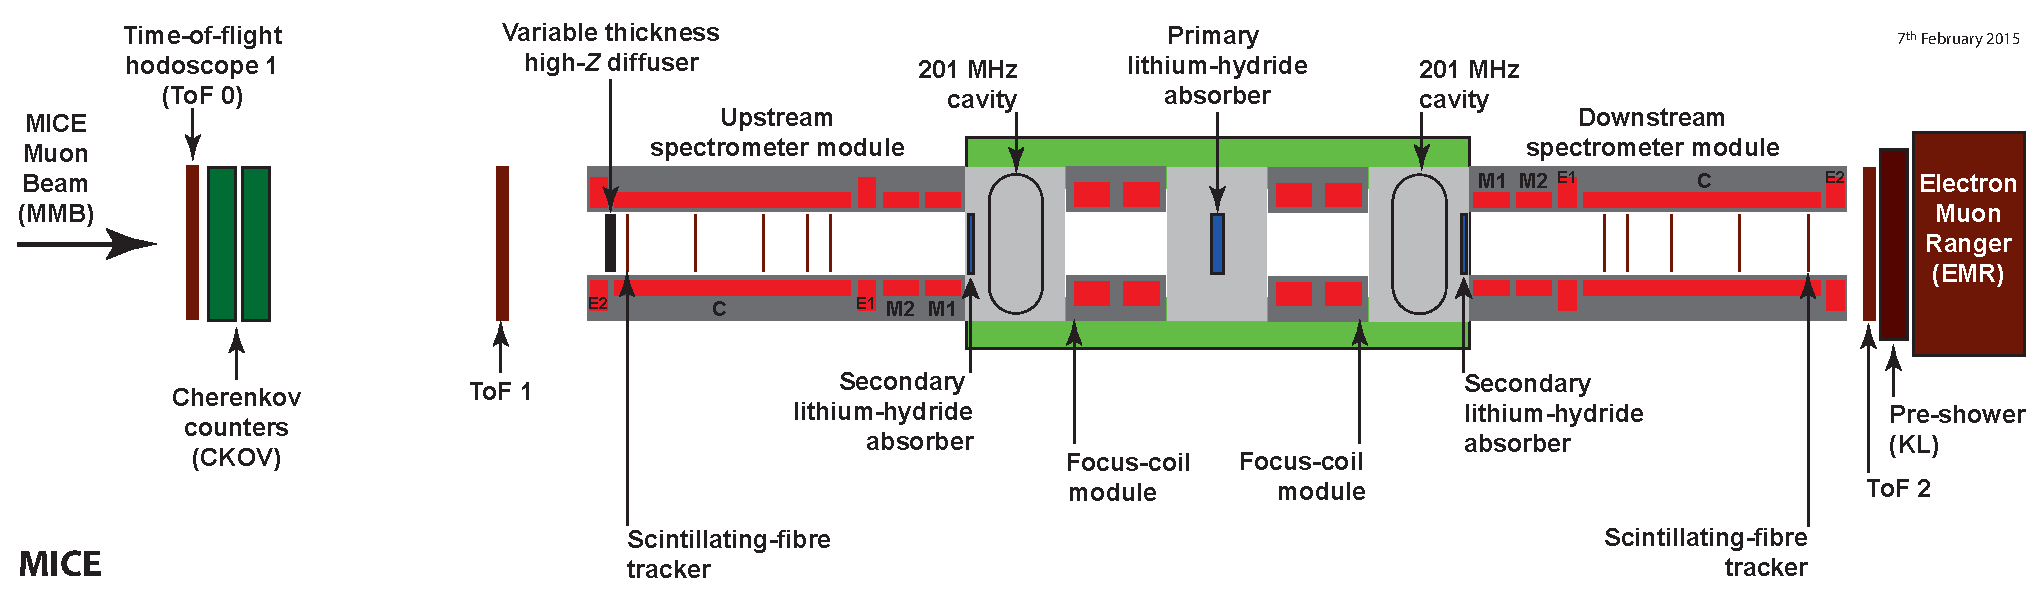
\includegraphics[width=1.0\linewidth]{01-MICE/Cooling-demo-labels.pdf}
      \caption{\label{fig:CoolingChannel} The beam diagnostics and cooling cell. Particle identification is provided by three time-of-flight stations, two threshold Cherenkov detectors and a downstream calorimeter composed of a pre-shower detector and electron-muon ranger. Emittance is measured upstream and downstream of the cooling cell by spectrometers. A diffuser is used to artifically increase the beam emittance prior to the cooling cell. Ionization energy loss occurs as the beam passes through the absorber modules, while longitudinal reacceleration is providing by radio frequency electric field cavities.}
    \end{center}
  \end{figure}

  MICE is based at the Science and Technology Facilities Council Rutherford Appleton Laboratory in the U.K., using the ISIS proton synchrotron to generate the muon beam~\cite{MiceTarget}.  The MICE beam line is described in detail in~\cite{MiceBeamline}. A schematic of the full MICE experiment is shown in figure~\ref{fig:CoolingChannel}. The beamline is instrumented with with two threshold Cherenkov detectors, three time-of-flight (TOF) stations and a downstream calorimeter. The cooling cell consists of three absorber modules and three radio frequency (RF) electric field cavities. Two high-precision trackers in a solenoidal field are used to measure the emittance change (see section~\ref{subsec:Trackers}).

  MICE is a staged experiment, that is, built and run in distinct steps. The first step of the programme, consisting of the muon beam line with particle identification, is now complete and results available in~\cite{MiceBeamline}. The present step of the program, which introduced the trackers and first absorber module, began taking data in 2015. % The demonstration of sustainable cooling, which includes longitudinal re-acceleration, will begin data taking in 2018.

%   \begin{figure}[tb]
%     \begin{center}
%       \includegraphics[width=0.75\linewidth]{01-MICE/BeamLineDEMOSans.pdf}
%       \caption{\label{fig:Beamline}The MICE Muon Beamline. A pion production target intercepts the protons of the circulating ISIS beam. Some of the subsequent pions are then captured by quadrupoles and guided down the beam line, passing through various PID detectors along the way, before delivery to the cooling cell itself. Emittance is measured immediately before and after the cooling cell using the scintillating fibre trackers.}
%       \end{center}
%   \end{figure}

  \subsection{The Scintillating Fibre Trackers}
  \label{subsec:Trackers}
  MICE is equipped with two identical, high precision scintillating-fibre (``scifi'') trackers, described in~\cite{MiceTrackers}. Each tracker is placed in a superconducting solenoid that provides a uniform field over the tracking volume. One tracker, TKU, is upstream of the cooling cell, the other, TKD, downstream.  Each tracker consists of 5 detector stations, labelled 1 to 5, as illustrated in figure~\ref{fig:Trackers}. TKU is orientated such that Station~5 sees the beam first, TKD is rotated by 180$^\circ$ such that Station~1 sees the beam first, thus, in both trackers, Station~1 is always nearest to the cooling cell (see figure~\ref{fig:CoolingChannel}).
  
  \begin{figure}[tbh]
    \centering
    \includegraphics[width=0.5\linewidth]{01-MICE/TrackerFrame.pdf} \hspace{2pc}%
    \includegraphics[width=0.35\linewidth]{01-MICE/TrackerPhoto.pdf}
    \caption{\label{fig:Trackers} Left: A schematic of the tracker carbon-fibre frame, showing the detector station positions.  The fibre planes are glued on to the upstream edge of the carbon-fibre station frames (shown in green). The longitudinal coordinate of the tracker coordinate system ($z_t$) increases as one moves from the fibre plane towards the station frame to which it is attached.  Right: A photograph of a tracker. The colour is due to the filtered lighting needed to protect the scintillating fibres. The intersecting lines visible on the station faces indicate the direction of the fibres in each plane.}
  \end{figure}

  Each station is formed of three planes of 350~$\mu$m scintillating fibres, orientated at 120 degrees to one another. The fibres in each plane are arranged in two layers offset with respect to each other (a ``doublet layer''), in order to give 100$\%$ coverage of the plane area as illustrated in figure~\ref{fig:DoubletLayer}. The doublet layer is glued on to a sheet of mylar. The fibres are collected into groups of seven for readout, each group forming a single channel, as illustrated in figure~\ref{fig:DoubletLayer}b. The planes, also known as views, are labelled $U$, $V$ and $W$. Plane $U$ is attached to the station frame directly, plane $W$ on to plane $U$, and plane $V$ on to plane $W$. The fibre-plane orientations are illustrated in figure~\ref{fig:FibrePlaneOrientation}. Each station is oriented such that the fibres in the $U$ plane are vertical. The fibres produce scintillation light when ionizing radiation passes through them. Clear-fibre light guides transport the scintillation light to visible light photon counters (VLPCs) that are operated at 9~$K$ in a cryostat. The signal from the VLPCs is digitised using front-end electronics developed by the D0 experiment~\cite{D0}. See~\cite{MiceTrackers} for details.

  \begin{figure}[tbh]
    \begin{center}
      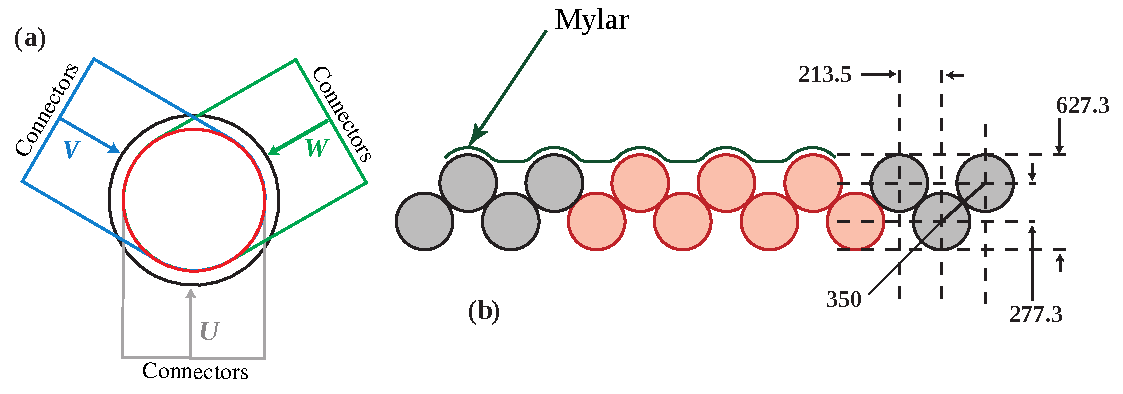
\includegraphics[width=0.85\textwidth]{01-MICE/doublet-layer.pdf}
      \caption{\label{fig:DoubletLayer}(a) Arrangement of the doublet layers in the scintillating fibre  stations. The outer circle shows the solenoid bore while the inner circle shows the limit of the active area of the tracker. The arrows indicate the direction that the individual 350\,$\mu$m fibres run. (b) Detail of the arrangement of the scintillating fibres in a doublet layer. The fibre spacing and the fibre pitch are indicated on the right-hand end of the figure in \,$\mu$m. The pattern of seven fibres shown in red form a single channel, which is readout via a clear-fibre light-guide. The sheet of mylar glued to the doublet layer is indicated. }
    \end{center}
  \end{figure}

  \begin{figure}[tbh]
    \centering
    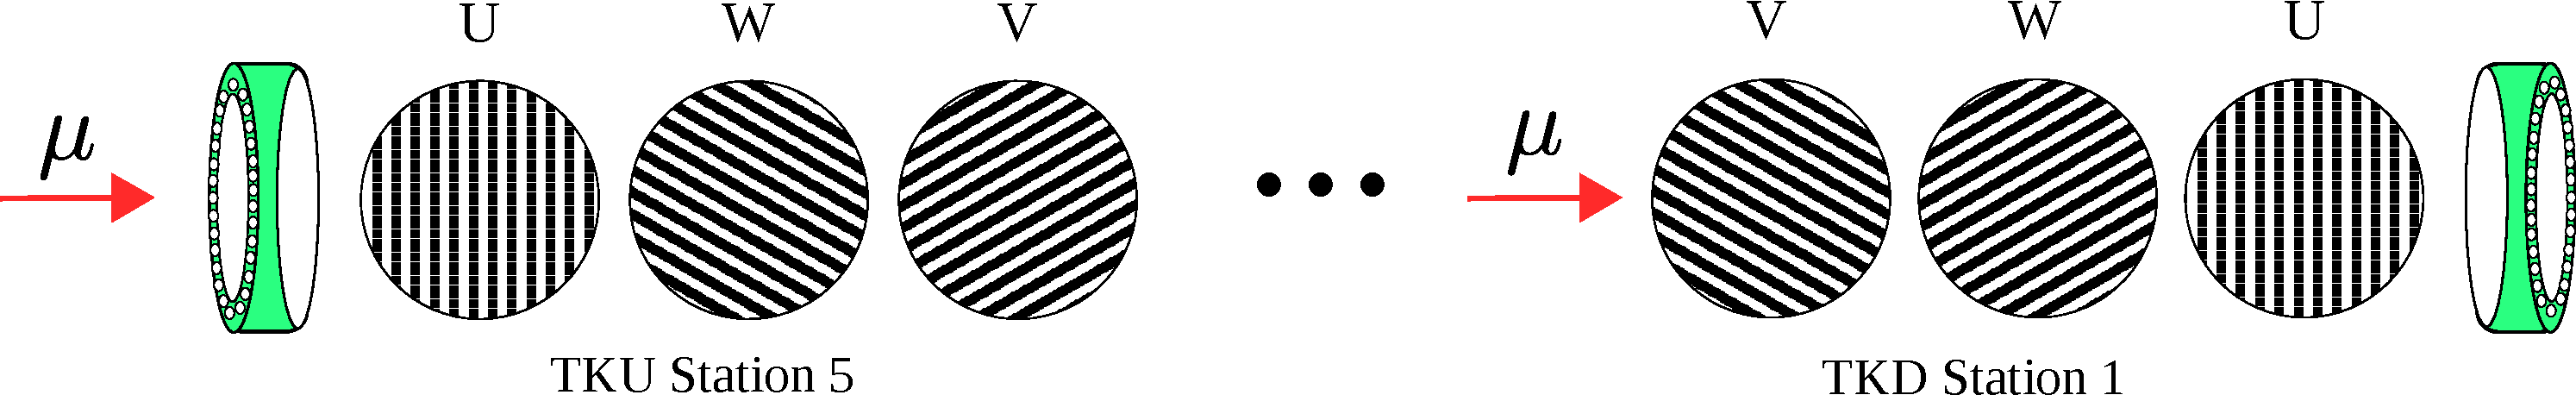
\includegraphics[width=0.95\linewidth]{01-MICE/FibrePlaneOrientation.pdf} \hspace{2pc}%
    \caption{\label{fig:FibrePlaneOrientation} The orientation of the fibres in each plane, as seen by the incoming beam, for both trackers. The green object is the station frame.}
  \end{figure}
\section{Coordinate systems and reference surfaces}
\label{sec:Coordinates}

  The planes, stations and trackers themselves each have a coordinate system defined on them which will be described in the following sections. Coordinates with subscript $p$ will refer to the plane coordinate system, $s$ to the station coordinate system and $t$ to the tracker coordinate system.

  \subsection{Channels and digits}
  The $V$ and $W$ planes each consist of 214 channels, labelled 0 to 213, while the $U$ plane has 212 channels, labelled 0 to 211.  The channel number increases from left to right if a plane is placed mylar side up, with the fibre readout pointing downwards, as illustrated in figure~\ref{fig:DoubletLayerOrder}.

  \subsection{Planes and clusters}
  \label{subsec:PlaneAndClusters}
  Each plane is assigned an integer known as the plane number: plane~$V$ is assigned~0; plane~$W$ is assigned~1; and plane~$U$ is assigned~2.  The plane reference surface is defined to be the flat plane that is formed by the outer surface of the mylar sheet. The measured position perpendicular to the direction of the fibres in each plane is labelled  $\alpha \in (v, u, w)$, defined to increase in the \textit{opposite} direction to the channel number with zero as the mid-point of the central channel. $\alpha$ is then given by $\alpha = \left(N_{CC} - N_{Ch}\right) \times d$, where $N_{CC}$ is the central channel number, $N_{Ch}$ is the channel number and $d$ is the channel width.
  
%   \begin{equation}
%    \alpha = \left(N_{CC} - N_{Ch}\right) \times p \times d
%   \end{equation}
% 
%   \noindent
%   where $N_{CC}$ is the central channel number, $N_{Ch}$ is the channel number, $p$ is the fibre pitch, that is twice the horizontal distance between neighbouring fibres ($2 \times 213.5 = 417$~mm), and $d$ is half the number of fibres in a channel, i.e. $3.5$ (see figure~\ref{fig:DoubletLayer}, it can be seen $p \times d$ is just the width of a channel).  
  
  The $z$ axis of the plane coordinate system is defined to be perpendicular to the plane reference surface and points in the direction from the mylar sheet towards the fibres. The direction in which the fibres run defines the final plane coordinate, $\beta$, completing a right-handed coordinate system. The origin of the $(\alpha, \beta)$ coordinate system is taken to be at the centre of the circular active area of the plane.

  \subsection{Stations and spacepoints}
  The station reference surface is defined to coincide with the reference surface of the $V$ doublet-layer. The station coordinate system is defined such that the $x_s$ axis is coincident with the $v$ coordinate (that is, $\alpha$ for the $V$ layer), the $z_s$ axis is coincident with the $z_p$ axis of the $V$ layer and the $y_s$ axis completes a right-handed coordinate system.

  \subsection{Trackers and tracks}
  Each tracker is assigned an integer known as the tracker number: TKU is assigned~0 and TKD is assigned~1. The tracker reference surface is defined to coincide with the reference surface of Station~1. The tracker coordinate system is defined such that the $z_t$ axis coincides with the axis of cylindrical symmetry of the tracker as shown in figure~\ref{fig:Trackers}. The tracker $z_t$ coordinate increases from Station~1 to Station~5. The tracker $y_t$ axis is defined to coincide with the $y_s$ axis of Station~1 and the tracker $x_t$ axis completes a right-handed coordinate system. 
  
  \begin{figure}[htb]
    \begin{center}
      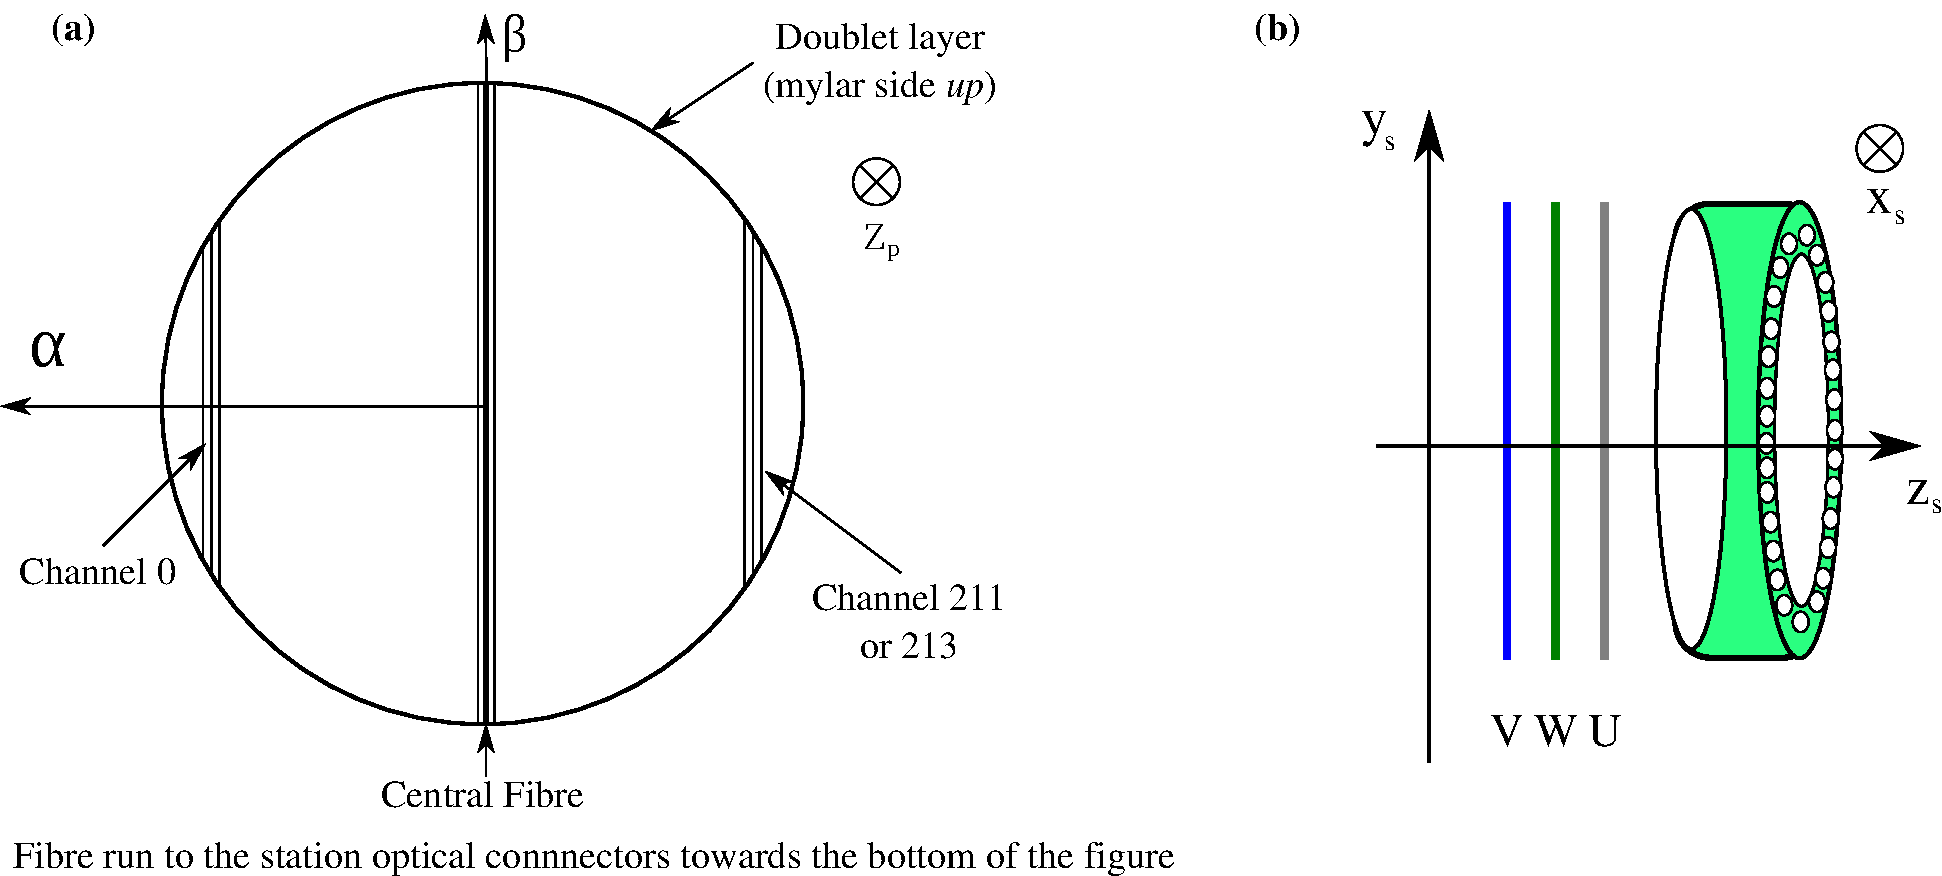
\includegraphics[width=0.9\textwidth]{02-CoordinateSystems/PlaneCoordinatesAndNumbering.pdf}
      \caption{\label{fig:DoubletLayerOrder} (a)~The channel numbering within a plane, and the $(\alpha, \beta, z_p)$ plane coordinate system (a right-handed system).  (b)~The fibre plane ordering with respect to the station body and the station coordinate frame (a right-handed system).  In TKU the beam approaches from the right, in TKD from the left. Note that $z_s$ is by definition equivalent to $z_p$ of the $V$ plane.}
    \end{center}
  \end{figure}


\section{The MAUS framework}
\label{sec:MAUS}
The tracker software is part of the MICE software framework, known as MAUS (MICE Analysis User Software)~\cite{MausIPAC11}. MAUS is used to perform Monte Carlo simulation and both online and offline data reconstruction. It is built using a combination of C++ and Python, with C++ being used for more processor-intensive tasks and Python being used more in the code presented to the user.  Simulation is based on GEANT4~\cite{GEANT4}, with analysis based on ROOT~\cite{ROOT}.  ROOT files are used as the primary output data format. %and the custom binary format written by the MICE data acquisition system (DAQ) is the primary input. 

MAUS programmes are defined in a Python script together with a configuration file.  This script allows the user to create programmes by combining different MAUS modules depending on the task at hand, following the Map-Reduce programming model~\cite{MapReduce}. The object passed between the modules is known as a ``spill'', representing the data associated with one spill of particles passing through the MICE beamline (see~\cite{BeamlineJINST}).  The modules come in four types: Input; Output; Map; and Reduce.  Input modules provide the initial data to MAUS, from a data file, or from the DAQ. Maps perform most of the simulation and analysis work and may be processed in parallel across multiple nodes.  Reducers are used to display output, such as for online reconstruction plots, and are capable of accumulating data sent from maps over multiple spills, but must be run in a single thread. Output modules provide data persistency.

The tracker software consists of 7 maps and a reducer. The maps cover: digitisation of Monte Carlo data; digitisation of real DAQ data; the addition of noise to Monte Carlo data; cluster reconstruction; spacepoint reconstruction; pattern recognition; and the final track fit. The reducer provides real time information on the tracker performance.  %The modules contain little code themselves but instead call C++ classes to perform the work.
\section{Data structure}
\label{sec:DataStructure}

\subsection{General MAUS, Monte Carlo and DAQ data structures}
\label{subsec:GeneralDataStructure}
A simplified schematic of the tracker data structure, with the relevant entries from the more general MAUS data structure, is shown in figure~\ref{figureDataStructure}.  All the objects listed represent container classes for different parts of the simulation, raw data and reconstruction.  The top-level object is the spill (see section~\ref{sec:MAUS}).  Within the spill the data is split into three branches: real-data from the DAQ; Monte Carlo data generated by simulation; and reconstructed data, which is formed from data in either the real or Monte Carlo branches. 

The reconstruction code makes no direct reference to the Monte Carlo information and has no way to distinguish real from simulated data, thus ensuring that they are treated equally.  The DAQ data is held in an object known as TrackerDAQ, within which the data is sub-divided according to the DAQ system it originated from.%Within TrackerDAQ data from the full MICE DAQ is stored in a VLSB object or, if the data originated in a cosmic-ray test DAQ, in a VLSB\_C object.

\begin{figure}[bt]
  \begin{center}
    \includegraphics[width=27pc]{04-DataStructure/DataStructureSimple2016.pdf}
    \caption{\label{figureDataStructure}The tracker software data structure and relevant MAUS data structure.  The spill is the top level object below which branches hold real-data, MC data and reconstructed data objects. When an object owns the memory of a set of other objects, these are held as standard vectors of pointers. When an object contains cross links to another set of objects, without owning their memory, these are held as a ROOT TRefArray of pointers. MC = Monte Carlo, SPR = Straight Pattern Recognition, HPR = Helical Pattern Recognition.}
  \end{center}
\end{figure}

The Monte Carlo event holds data on ``scifi hits'' produced by tracks passing through the fibre planes and any noise hits originating in those planes. The scifi hit is implemented as a class based on the generic hit-class template from which all the different MICE detector-hit classes are derived.  Other relevant data held in the Monte Carlo event, though not part of the tracker data structure, include the simulated tracks and ``virtual hits'' which contain information of the track state at their location. Such data is used to evaluate the reconstruction performance against the original simulated data (see section~\ref{sec:Performance}).

\subsection{Tracker reconstruction data structure}
\label{subsec:TrackerReconDataStructure}
The reconstructed data for the tracker is held in the ``scifi event'' class.  This contains vectors of the following container classes that represent the higher-level reconstructed tracker-data:

\begin{itemize}
  \item ``Digits'' contain the analogue-to-digital converter (ADC) counts (real or simulated) from the readout of a single channel in response to an incident track;
  \item ``Clusters'' are groups of neighbouring digits arising from a particle crossing one or two channels;
  \item ``Spacepoints'' group clusters from adjacent detector planes to give a point in tracker coordinates;
  \item ``Straight pattern recognition tracks'' group together spacepoints from different tracker stations when the track that introduced the hits was straight (i.e. when the magnetic field is off); %The track parameters given in eqn.~\ref{eqn:StraightTrackParameters} are also stored;
  \item ``Helical pattern recognition tracks'' group together spacepoints from different tracker stations when the track that introduced the hits was helical (i.e. when the magnetic field is on); %The track parameters given in eqn.~\ref{eqn:HelicalTrackParameters} are also stored;
  \item ``Scifi tracks'' hold the final Kalman fit parameters of the particle track; and
  \item ``Trackpoints'' hold the fit parameters at each detector plane, including the momentum and position of the track.
\end{itemize}

Each of these objects is stored directly in the scifi event object (the event ``owns'' the required memory), with the exception of trackpoints which are stored in the associated scifi tracks.  Each higher-level object also contains cross links in the form of pointers back to the objects within the scifi event which were used to create it. In this manner all higher-level objects can be traced back to the original digits.  In the case of a Monte Carlo run the digits themselves are linked via an ID number and lookup table back to the scifi hits used to produce them. The ID is defined as \textit{tspc}, where \textit{t} is the tracker number, \textit{s} is the station number, \textit{p} is the plane number and \textit{c} is the channel number (given with three numerals e.g. 010 for channel 10).  This structure means the reconstruction branch has no direct reference to the Monte Carlo data.
\section{Geometry}
\label{sec:Geometry}
  
  \begin{table} [tbp]
  \begin{center}
  \begin{tabular} {|c|c|c|c|c|c|}
    \hline
    \multicolumn{6}{|l|}{Tracker 1 offsets in mm} \\
    \hline
    & Station 1 & Station 2 & Station 3 & Station 4 & Station 5 \\
    \hline
    X & 0.0 & -0.5709 & -1.2021 & -0.5694 & 0.0 \\
    Y & 0.0 & -0.7375 & -0.1657 & -0.6040 & 0.0 \\
    Z & -1099.7578 & -899.7932 & -649.9302 & -349.9298 & 0.0 \\
    \hline
    \hline
    \multicolumn{6}{|l|}{Tracker 2 offsets in mm} \\
    \hline
    & Station 1 & Station 2 & Station 3 & Station 4 & Station 5 \\
    \hline
    X & 0.0 & -0.4698 & -0.6717 & 0.1722 & 0.0 \\
    Y & 0.0 & 0.0052 & -0.1759 & -0.2912 & 0.0 \\
    Z & -1099.9026 & -899.009 & -650.0036 & -350.0742 & 0.0 \\
    \hline
  \end{tabular}
  \caption{\label{tab:CMM} The position of the tracker stations with respect to the tracker reference surface as measured by the coordinate measuring machine.}
  \end{center}
  \end{table}
  
  The position of each tracker station was determined with respect to the tracker reference surface using a coordinate measuring machine (see table~\ref{tab:CMM}). The station positions are stored in the MICE configuration database (CDB). The CDB is a bi-temporal database, alterations being tracked by date and run number. Information is stored in the CDB as a collection of XML files which are translated into the native MAUS format ``MiceModules'', at run-time.  The MiceModules are text documents and contain all the information needed to simulate the various MICE systems and detectors.  MAUS uses the same geometry descriptions for both simulation and reconstruction. 
  
  In the description of the geometry MAUS adopts a passive rotation convention to be consistent with GEANT4.  The active volume of each tracker is given by a cylinder of 150~mm radius, which is used to define the fiducial volume for the reconstruction. Alignment of the individual tracking stations and the trackers themselves to the solenoid axis has been completed using real-data.
  
  % The only differences between the Monte Carlo and the real geometries relate to non-active portions of the experiment and field mapping. In particular, only the Monte Carlo geometry contains the epoxy resin, which was used in securing the individual scintillating fibres to the tracker station body, and the mylar sheets to support each doublet-layer. The carbon fibre body of the trackers have not been included in either the real or Monte Carlo geometries as their effect on the beam is expected to be minimal.
  
  
\section{Simulation}
\label{sec:Simulation}

The simulation of the trackers makes use of the GEANT4 standard physics libraries to describe particle motion through the fields and material of the beamline. The trackers are simulated on a per-fibre basis and arranged into doublet-layer planes (as described in section~\ref{subsec:Trackers}). As particles pass through the fibres scifi hits are generated, containing the energy deposited in the fibre. 

The scifi hits are converted by the MAUS module used to digitise simulated tracker data (MapCppTrackerMCDigitisation) into to a number of photoelectrons (NPE) produced in the tracker VLPCs by means of a simple conversion factor. At this point the NPE values are non-integers, and are quantised simply by rounding down. These NPE values are then ``smeared'' to simulate the detector response (the electron avalanche effect in the VLPCs). The smearing process involves modeling this response as a Gaussian, the mean being given by the quantised NPE value and the width being determined from data. Once the smearing is complete the signal is split into $2^8$ bins to represent the sampling size of the 8 bit ADCs. The simulated ADC counts are then used together with the measured calibration for each channel to give a final NPE value.

It is also possible to add noise to digitisation process by the addition of an extra MAUS module (MapCppTrackerMCNoise). Noise may arise in the signal from thermally excited electrons within the VLPCs, known as ``dark count''. The dark count is a stochastic process described by a Poisson distribution. Physically the rate can be changed by altering the bias voltage on the VLPCs, with a target dark count rate of 1 NPE in 1.5\% of the fibres per particle trigger, with higher numbers of NPE having a smaller probablility following the Poisson distribution. The effect is modelled in the software and used to introduce additional photoelectrons to the simulated signal prior to the quantisation and smearing stage. 

Once the final NPE value has been calculated it is combined with the channel number to form a digit object. The digits are then added to the scifi event and sent on to the reconstruction modules.


% The MAUS framework invokes a beamline module to generate a simulated beam, according to pre-defined user parameters.  A particle incident upon a tracker fibre is stepped through, in accordance with the defined parameters. GEANT4 is invoked in each of these steps in determining the resulting momentum change of the particle and the magnitude of energy  deposited into the fibre.  These values are recorded individually, the current step used in determining where the next step is taken, and recorded before the next step is processed.  After a defined number of particles have been generated and stepped through the experiment the results are collected into a MICE spill and sent to the tracker MC module for processing.  

% A single interaction with a scintillating fibre is simulated by many steps through the material and the figure for any one step is not limited to integer values.  The raw NPE from every step through the fibre is summed and feed into the simulation of noise in the tracker electronics (see section \ref{subsec:Noise}).

%   \subsection{Noise}
%   \label{subsec:Noise}
%   The MC noise simulation consist of two modules, false signal due to thermally excited electrons within the VLPC cassettes and a smearing due to random noise in the tracker electronics.  This is in addition to noise introduced by particle decays handled outside of the tracker MC by the GEANT4 simulation.
%   
%   Simulation of the thermally excited electrons is performed before the smearing simulation.  The dark count is an uncorrelated process that is selected to occur with a magnitude of 1.0 PE in 1.5$\%$ of a data taking window.  Actual rate is determined by the setting of the voltage bias in the VLPC cassettes which as a direct effect on the final signal size.  The process is described as a Poisson distribution.  Studies are under way to understand this effect in each cassette. 
%   
%   The results from the GEANT4 physics simulation and the Poisson dark count simulation are combined and smeared to determine the final NPE signal.  The signal from the GEANT4 simulation can take any value, however, it is unreasonable to expect anything other than an integer number of photons, as such this incoming signal is changed to its nearest integer value. The value is smeared as described by a Gaussian with a sigma derived from a study of carried out in May 2012 of a single station in beam.
%   
%   The smeared result is then fed through a process that simulates the effects of the analogue to digital converters (ADCs).  This process serves to chop the information up into bins of $2^8$ discreet values.  The exact values of these bins is determined from the tracker calibrations and varies with the with the channel placement into the electronics.  Overflows are equivalent to the maximum signal.  
\section{Reconstruction}
\label{sec:Reconstruction}
The reconstruction process begins with either real or simulated data and proceeds to reconstruct progressively higher-level objects step-by-step, culminating in scifi tracks and trackpoints. The digits, real or simulated, are passed to the same MAUS module (MapCppTrackerRecon) and the reconstruction proceeds identically for either case from that point. The reconstruction process is illustrated in figure~\ref{fig:DataFlow} and is described in the sections that follow.

\begin{figure}[tbh]
  \begin{center}
    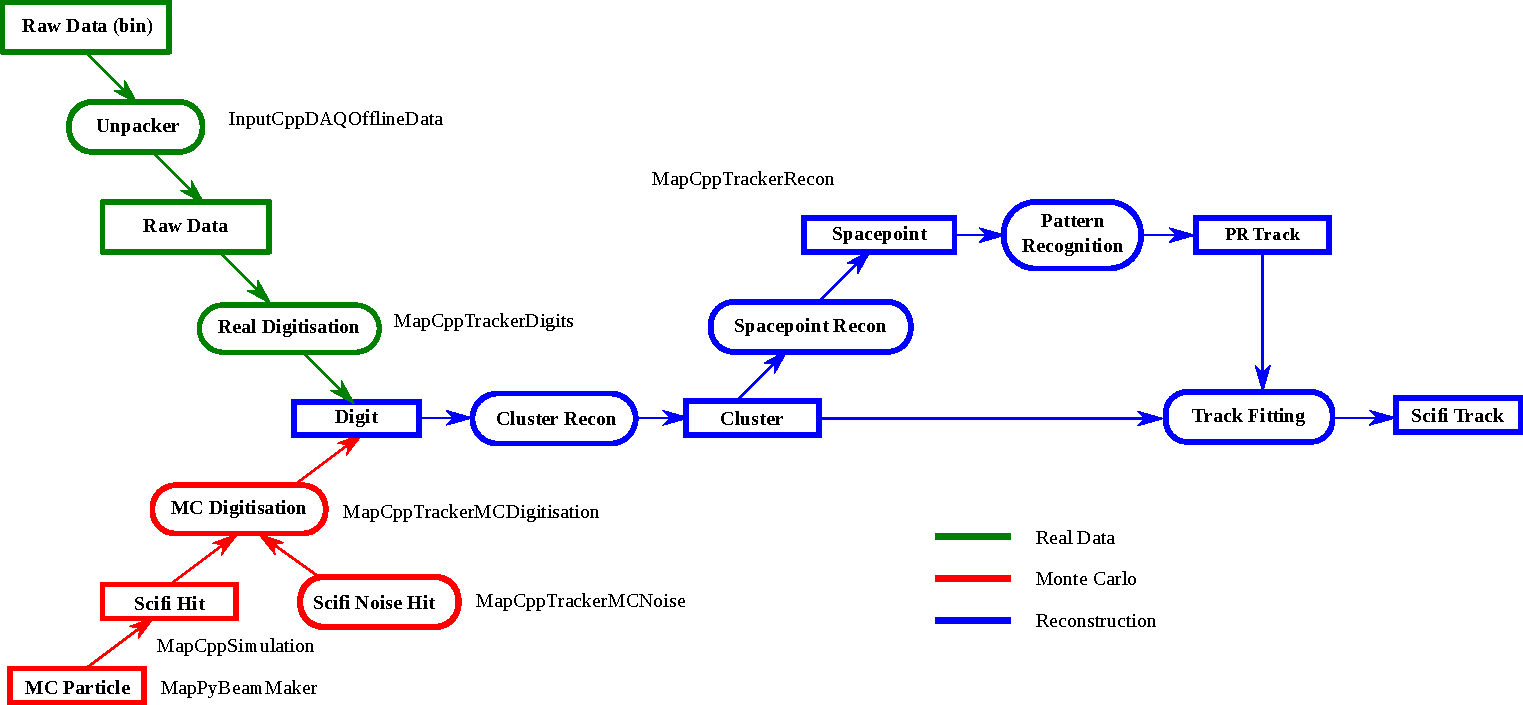
\includegraphics[width=0.95\linewidth]{07-Reconstruction/DataFlow2014.pdf}
    \caption{\label{fig:DataFlow} The reconstruction data flow. Data originates either from simulated or real-data, the two branches merge after digitisation, after which the reconstruction proceeds identically.  The relevant MAUS modules for each step are indicated.}
  \end{center}
\end{figure}

  \subsection{Digitization}
  \label{subsec:Digitization}
  For real-data the signal from the tracker ADCs is recorded by the DAQ system.  Channel-by-channel calibration constants are used to convert the ADC value to a signal in NPE and the DAQ channel number to tracker channel number.  This information is then used to form a digit.  The analogous process for Monte Carlo data is described in section~\ref{sec:Simulation}.

  \subsection{Clustering}
  \label{subsec:Clustering}
  The clustering algorithm loops over every combination of pairs of digits in a scifi event and combines any that occur in neighbouring channels. In the case of multi-digit cluster, the unweighted average channel value is used to define the plane coordinate, $\alpha$, and the NPE is summed.

  \subsection{Spacepoint Reconstruction}
  \label{subsec:SpacepointReconstruction}
  For each station the constituent planes are searched for clusters that can be used to form a spacepoint. Spacepoints are constructed from clusters from all three planes (a triplet spacepoint) or for any two out of the three planes (a doublet spacepoint).

  To determine which clusters from each plane originate from the same track, Kuno's conjecture~\cite{MiceTrackers} is used: for a given triplet spacepoint the sum of the channel numbers of each cluster will be a constant.  So if $n^u$, $n^v$ and $n^w$ are the fibre numbers of the clusters in $u$, $v$ and $w$ and $n^u_0$, $n^v_0$ and $n^w_0$ are the corresponding central channel numbers. Three clusters form a space point if:
  \begin{equation}
    | (n^u + n^v + n^w) - (n^u_0 + n^v_0 + n^w_0) | < K \, .
  \end{equation}
  where $K$ is a constant, taken by default to be 3.0.
  
  Once all triplet spacepoints have been found, doublet spacepoints are created from pairs of remaining clusters, the only selection criteria applied being that the crossing point of the two channels is within the tracker radius. 
  
  Spacepoint positioning is determined from the cluster measurements, $\alpha$ (see section~\ref{subsec:PlaneAndClusters}) and the known plane orientations for those measurements. All clusters selected as belonging to the same spacepoint must interesect. Using two clusters the second plane coordinate $\beta$ may be calculated using knowledge of the plane orientations. This then expresses the crossing point in the $(\alpha, \beta)$ coordinate system, which can be simply rotated into the station $(x, y)$ coordinate system. In the case of a triplet spacepoint three crossing points are present, the average of which is used to define the final spacepoint position.

% For overlapping clusters:
%   
%     \begin{equation}
%     \begin{pmatrix}
%     \alpha_1 \\ \beta_1
%     \end{pmatrix} = R_{1}^{-1} R_2
%     \begin{pmatrix}
%     \alpha_2 \\ \beta_2
%     \end{pmatrix}
%     \end{equation}   
% \noindent

  % \subsubsection{Crossing Point Calculation}
  % \label{subsubsec:CrossingPointCalculation}

  \subsection{Pattern Recognition}
  \label{subsec:PatternRecognition}

  Pattern recognition is based on looping over different combinations of spacepoints and performing a fit using a linear least squares technique. There are separate algorithms for the straight track (no field) case and the helical track case.

   \subsubsection{Helical Pattern Recognition}
   \label{subsubsec:HelicalPatternRecognition}

   %The helical pattern recognition is performed in cylindrical co-ordinates $(r, \phi, z)$ where the turning angle $\phi$ defined for $0 \rightarrow \infty$ is distinguished from $\phi '$ the reduced turning angle defined for $0 \rightarrow 2\pi$. 
   
   The helical pattern recognition is performed in cylindrical co-ordinates $(r, \phi, z)$, where $r$ is the helix radius, $\phi$ the turning angle in the transverse plane, and $z$ is the longitudinal coordinate. An additional coordinate, $s$ the distance the particle travels in the transverse plane, is also defined. The helix is then parameterised by: the circle centre $x_c$, $y_c$ and the radius, $r$, in the transverse plane; $s_0$ the value of $s$ where the helix crosses the reference plane; and $t_s = ds/dz$, which describes the tightness of the coiling. %$\phi_0$, the angle of the track as it crosses the tracker reference plane, equivalent to $s_0$, is also used. 

   To find a track one spacepoint is selected from each station and a circle is fitted in the $(r, \phi')$ projection. If the $\chi^2$ of this fit is sufficiently small (by default less than 15.0 multiplied by the number of degrees of freedom, NDF) then the value of $\phi$ is used to generate $s$ and a straight line fit is performed in the $(z,s)$ plane, and if the $\chi^2$ in this projection is also small (by default less than 4.0 multiplied by the NDF) the track is accepted as a track candidate. Once all the different possible combinations of spacepoints have been tried the track candidate with the lowest combined $\chi^2$ from the fits is selected as the true track. Once every possible track with a spacepoint in all 5 stations has been found, the procedure is repeated looking for tracks with spacepoints in only 4 of the 5 stations. %$\phi$ itself is determined from $\phi'$ by exploiting the different distances in $z$ between successive tracker stations.  The change in $\phi$ between the hits in any two stations, divided by the distance between those stations, gives a constant which is the same for any pair of hits.  This can then be used to infer the true values of $\phi$.
   %TODO Define small
   
   %Tracks with momentum almost parallel to the solenoid axis (i.e. with low transverse momentum, $p_T$) will not suffer an appreciable bend and will not be found by the helix search and so any spacepoints remaining after the helical tracks have been found are passed to the straight track finding algorithm.

    \subsubsection{Straight Line Pattern Recognition}
    \label{subsubsec:StraightLinePatternRecognition}

    % Straight lines are fitted to the spacepoints when there is no magnetic field and on any spacepoints remaining after the helix fit is complete. The latter is to identify tracks with a small $p_T$ which are not bent sufficiently in the magnetic field to form a recognisable helix (it has been observed from Monte Carlo studies that the efficiency of the helix finding algorithm begins to tail off for tracks with $p_T < 10 MeV/c$).

    The straight-track finding is performed in Cartesian coordinates. The track parameters are $(x_0, y_0, t_x, t_y)$ where: $(x_0$, $y_0)$ is the position the track crosses the tracker reference surface; $t_x = dx/dz$; and $t_y = dy/dz$. Two spacepoints are chosen in the outer stations and a road is created between them. Any spacepoints in the road are fitted in the $(x,z)$ and $(y,z)$ planes. If the $\chi^2$ of the fits is small (by default less than 4.0 multiplied by the NDF) a candidate track is formed. Once all possible spacepoint combinations have been tried the track candidate with the lowest $\chi^2$ is selected. As in the helical case, following the completion of the full 5 point track search, tracks with spacepoints in 4 out of the 5 stations are searched for. For the straight case only, following the completion of the search for 4 point tracks, a search is also made for tracks with spacepoints in only 3 out of the 5 stations. 

   \subsection{Track Fit}
   \label{subsec:FinalTrackFit}
   The final track fit was implemented using a track-orientated Kalman filter~\cite{Fruhwirth,Billoir}, which can be shown to be an optimal linear fitter, that takes into account all correlations and measurements, for a linear system. The Kalman filter is an iterative algorithm that incrementally propagates an estimate of the current track state between measurement planes, using measurement information to ``filter'' the state, improving the estimate of the track state.
   
   For the helical track fit, the system is only approximately linear, hence an extended Kalman filter~\cite{Goodwin} was implemented which analytically propagates the track states between measurements, while the covariance matrices are propagated using a first-order linear approximation to the non-linear system.

   Pattern recognition provides a set of clusters that are associated with a track, which passed the selection criteria, and a parameterisation of that track based on a least squares fit to the points by a helix or a straight line as appropriate. The track parameters calculated from the least squares fit are used to provide the seed for the Kalman fit and the raw cluster information is used as the measurement data. The flexibility of the Kalman algorithm permits the effects of individual planes (multiple coulomb scattering MCS, and energy loss) and the material effects of the helium gas within the tracker to be accounted for between each measurement point.
%      \subsubsection{Kalman Filtering}
% 
%      The track is modelled as a discrete state space function of $z$ (the direction of the beam), indicated by the subscript, $k$, where each tracker plane corresponds to a trackpoint and contains a measurement and a track state. Equation~\ref{equ:kalman_system_equation} describes how the true state space vector, $\mathbf{x}_{k,t}$, is assumed to propagate to a subsequent measurement plane. The matrix, $\mathbf{F}_k$, is the Kalman Propagator and describes the first order description of the propagation between measurement planes. $\mathbf{w}_k$ represents some ``process noise'', which may affect the system between the two measurement planes and is assumed to be Gaussian distributed white noise.
%     \begin{equation}
%       \mathbf{x}_{k,t} = \mathbf{F}_{k-1}\mathbf{x}_{k-1,t} + \mathbf{w}_{k-1}
%       \label{equ:kalman_system_equation}
%     \end{equation}
%     \begin{equation*}
%       \textrm{exp}(\mathbf{w}) = 0 \quad\quad \textrm{and} \quad\quad \textrm{cov}(\mathbf{w}) = \mathbf{Q}
%     \end{equation*}
%      
%      The tracker measurements are interpreted in a different state space to the track, allowing measurements of any dimension to be used to filter the track. Equation~\ref{equ:kalman_measurement_equation} describes how the true track state is ``measured'' to be transformed into the measurement space. The matrix, $\mathbf{H}_k$, is the Kalman Measurement Matrix and describes, to first order, the transformation from track state space to the measurement state space. $\mathbf{\varepsilon}_k$ represents some ``measurement noise'' which may smear the measurement of the true state space, it is also assumed to be Gaussian distributed.
%     \begin{equation}
%       \mathbf{m}_k = \mathbf{H}_kx_{k,t} + \mathbf{\varepsilon}_k
%       \label{equ:kalman_measurement_equation}
%     \end{equation}
%     \begin{equation*}
%       \textrm{exp}(\mathbf{\varepsilon}) = 0 \quad\quad \textrm{and} \quad\quad \textrm{cov}(\mathbf{\varepsilon}) = \mathbf{V}
%     \end{equation*}
% 
%     For each measurement plane that contains a measurement, the current estimate for the track state vector is ``filtered'' using the measurement information. This is achieved using the residual between the estimate for the track state and the measurement data, in the measurement state space. Equation~\ref{equ:kalman_state_filtered} describes how the predicted state vector, $\mathbf{x}_{k}^{k-1}$ is filtered using the Kalman Gain Matrix, $\mathbf{K}_k$, to produce the filtered track estimate, $\mathbf{x}_k$. Equation~\ref{equ:kalman_gain_matrix} defines the Kalman Gain Matrix.
%     \begin{equation}
%       \mathbf{x}_k = \mathbf{x}_k^{k-1} + \mathbf{K}_k ( \mathbf{m}_k - \mathbf{H}_k \mathbf{x}_k^{k-1} )
%       \label{equ:kalman_state_filtered}
%     \end{equation}
%     The predicted covariance matrix, $\mathbf{C}_k^{k-1}$, is filtered in a similar  fashion to produce the filtered covariance matrix, $\mathbf{C}_k^{k}$, as described in equation~\ref{equ:kalman_covariance_filtered}:
%     \begin{equation}
%       \mathbf{C}_k = ( \mathbf{I} - \mathbf{K}_k \mathbf{H}_k ) \mathbf{C}_k^{k-1}
%       \label{equ:kalman_covariance_filtered}
%     \end{equation}
%     The Kalman Gain matrix is calculated by:
%     \begin{equation}
%       \mathbf{K}_k = \mathbf{C}_k^{k-1} \mathbf{H}_k^\mathsf{T} (\mathbf{V}_k + \mathbf{H}_k \mathbf{C}_k^{k-1} \mathbf{H}_k^\mathsf{T})^{-1}
%       \label{equ:kalman_gain_matrix}
%     \end{equation}
% 
%     The sequence of prediction and filtering is repeated for all the measurement planes, starting from station~5, plane~2, where the predicted state vector and covariance matrix is determined from the pattern recognition fit parameters, to station~1, plane~0, the reference plane. Once the reference plane has been reached, the state vector will have been sequentially filtered using all the measurements in turn to create the optimal estimate of the track state at that plane. The fit can then be smoothed, whereby the optimal state vector is propagated in reverse down the length of the track, such that all the subsequent measurements can be used to re-adjust previous state vector estimates. This is described in~\cite{Fruhwirth}


%     \subsubsection{The MAUS Kalman Filter Implementation}
    The Kalman filter was written entirely from scratch. In order to make the implementation flexible and re-usable the core algorithm was implemented without any dependencies on phase-space dimensions or physical effects. % Due to this only the system specific functionality need be provided for a complete implementation.
    The principal components of the implementation are: propagation routines for both helical and straight tracks; a measurement routine that transforms the track state-space into the measurement state-space; and approximations for the process and measurement noise.
    
    The measurements correspond to individual clusters, hence the parameter $\alpha$ (see section~\ref{subsec:PlaneAndClusters}) forms a one-dimensional measurement state. The measurement noise corresponds to the statistical spread of measurements of width $w$, within a single channel in the tracker readout. If the channel is modelled as a top-hat function, the variance of the function is $w^2/12$. Therefore the measurement noise was taken to be $w/\sqrt{12}$ for all clusters.

    The process noise was implemented as a combination of MCS and energy straggling. The energy loss is calculated using the Bethe formula, for the most probable energy loss, and applied during the propagation stage. The noise term itself is calculated per increment as an RMS scattering angle using an implementation of the Highland formula (equation~\ref{equ:highland_formula}), in a fashion almost identical to the GEANT4 implementation:
    \begin{equation}
      \theta_{RMS} = \frac{13.6\textrm{MeV/c}}{\beta c p} Z \frac{x}{X_0}\left( 1 + 0.038 \ln\left(\frac{x}{X_0} \right)\right)
      \label{equ:highland_formula}
    \end{equation}
    where $\theta_{RMS}$ is the RMS scattering angle through a finite length of material, $\beta c$, $p$ and $Z$ are the velocity, momentum and charge of the particle in question, $x$ is the distance travelled and $X_0$ the radiation length of the material. Although the RMS scattering angle does not form a Gaussian distribution, the first order approximation is believed to be sufficient.

    In contrast to Pattern Recognition, the Kalman Filter uses a different state space model, ($x$, $p_x$, $y$, $p_y$, $q/p_z$) rather than ($x_c$, $y_c$, $r$, $s_0$, $t_s$). This permits the energy loss and multiple coulomb scattering to be modelled linearly and implmentated using a more simple set of algorithms. The longitudinal components however are less well modelled due to small angle scattering, such that the reconstruction of $p_z$ from the final track fit is sensitive to the accuracy of the pattern recognition stage.

%    \subsubsection{Goodness of fit}
%    For each fitted track, a test statistic is computed, which is the $\chi^2$ sum over all the trackpoints. It is calculated by $\chi^2\sum_{k=0}^{k=n}\chi_k^2$ where each chisquared update is given by $\chi_{k}^{2}=\mathbf{r}_{k}^{T}\mathrm{R}_{k}^{-1}\mathbf{r}_{k}$: where $r_{k}$ is the residual computed from the filtered state vector. $r_{k}=\mathbf{m}_{k}-\mathrm{H}_{k}\mathbf{a}_{k}$: where $\mathbf{m}_{k}$ is the $k^{th}$  measured point; $\mathbf{a}_{k}$ is the best Kalman estimate of track state vector at the $k^{th}$ intersection point and $\mathrm{H}_{k}$ is the matrix which projects the state vector of the track into the measurement space. $\mathrm{R}_{k}$ is the covariance matrix of the residuals and is given by  $\mathrm{R}_{k}=\mathrm{V}_{k}-\mathrm{H}_{k}\mathrm{C}_{k}\mathrm{H}_{k}^{T}$ where $\mathrm{V}_{k}$ is the measurement covariance matrix and $\mathrm{C}_{k}$ is the projected variance matrix. This definition of  $\chi^{2}$  takes into account correlations in the measurement predictions and, combined with the number of degrees of freedom of the track fit, is used to generate a {\it p-value} for the track, which we use as a measure of fit quality.


%\begin{equation}
%\chi_{k}^{2}=\mathbf{r}_{k}^{T}\mathrm{R}_{k}^{-1}\mathbf{r}_{k}.
%\end{equation}





  

\section{Performance}
\label{sec:Performance}

  A Monte Carlo simulation was used to determine the efficiency and resolution of the reconstruction algorithms. It was necessarily Monte Carlo based in order to compare the reconstructed events to the simulated ``truth'', thereby highlighting any inefficiencies and inaccuracies.

  The fitted transverse positions, $(x,y)$, and momenta, $(p_x, p_y, p_z)$, were compared to the Monte Carlo truth on an event-by-event basis. The reconstruction of the Monte Carlo data followed the same requirements that are used for the real-data reconstruction. The Monte Carlo truth data was stored at every tracker plane (via virtual hits) to permit a direct comparison with the reconstructed data. All comparisons were made at the tracker reference surface. %the designated measurement location with the MICE cooling channel.

  An artificial beam was generated with uniform distributions for both the longitudinal and transverse momenta. This ensured that the results were not biased by the incoming beam distribution and that the full reconstructible phase-space was probed with equal statistics. In order to remove unwanted ``non-physical'' particles, a cut was placed on the Monte Carlo truth data during the analysis phase to eliminate tracks with a large $p_t/p_z$ ratio. Tracks with a ratio greater than $0.5$ (that is, a $45^\circ$ angle with respect to the $z$ axis) were rejected from the analysis.
  
  \subsection{Kuno's Conjecture}
  \label{sec:performance:kunos_conjecture}
  
  All clusters selected to form triplet spacepoints should follow Kuno's conjecture (section~\ref{subsec:SpacepointReconstruction}). A plot showing the sum of the channel numbers for the clusters in each spacepoint is shown in figure~\ref{fig:kuno}. As expected the sum of the channel numbers for all the clusters in a spacepoint is constant to very good approximation.  The small variation arises from the fact that in real data the channels overlap by approx $1/11^{\mathrm{th}}$, however, in the Monte Carlo digitiser a $50\%$ overlap is assumed. This effect is only seen when there is at least one 2-digit cluster. When only 1-digit clusters are allowed the discrepancy is removed completely.

  \subsection{Track Finding Efficiency}
  \label{sec:performance:track_finding}

  For every simulated event, the number of tracks expected was calculated from the Monte Carlo truth. If a simulated track crossed enough tracker planes to create a sufficient number of spacepoints (3 for straight tracks and 4 for helical tracks), a reconstructed track was expected. The parameters of the reconstructed tracks were compared to the expected track parameters. The efficiency of track finding as a function of the true longitudinal and transverse momentum is shown in figure~\ref{fig:track_efficiency}. High efficiency is observed across the momentum range, with the exception of dip at low transverse momentum ($p_t <$ 5~MeV/c) and a smaller dip in the high transverse momentum, low longitudinal momentum region. The former effect may be an artifact of the track model at small track radii. Both effects are under investigation in order to optimise the efficiency in these regions.

  %Once the the Monte Carlo tracks have been identified, the expected number of trackpoints can be calculated by examining the number of tracker planes that the simulated track crossed. Comparing the number of trackpoints in each reconstructed track to the expected number for each simulated track permits the efficiency of finding the correct number of trackpoints to be calculated. Figure~\ref{fig:tp_efficiency} shows the trackpoint finding efficiency as a function of longitudinal and transverse momenta.

  \subsection{Position and Momentum Resolution}
  \label{sec:performance:resolutions}
  
  %Position residuals are shown in figures~\ref{fig:XResidKalman} and \ref{fig:YResidKalman}, and the momentum residuals in figures~\ref{fig:PtResidKalman} and \ref{fig:PzResidKalman}.  The position reconstruction can be seen to agree with the Monte Carlo truth to high precision in both the upstream and downstream trackers. The momentum residuals currently display some systematic effect which is due to uncertainty in the determination of energy loss within the tracker and the accuracy of the pattern recognition parameters.
  
  The $\chi^2$ per degree of freedom for the track fits, used to provide the position and momentum determinations, are shown in figure~\ref{fig:track_chisq}. 
  The position residuals, shown in figures~\ref{fig:XResidKalman} and \ref{fig:YResidKalman}, are consistent with the expected measurement resolutions for a combined fit. The transverse momentum resolution, shown in figure~\ref{fig:PtResidKalman}, is consistent across the range of the sensitive phase-space at $\sim$0.9~MeV/c in both trackers. The longitudinal momentum shown in figure~\ref{fig:PzResidKalman}, an intrinsically more difficult measurement for the tracker, retains an acceptable spread of ${\sim4}$~MeV/c in both trackers. There is however a small systematic effect visible in the momentum distributions. This will be removed by matching the tracks to the instrumentation upstream and downstream of the tracker modules.

  In order to produce these plots, a requirement that there was a cluster within the reference plane was applied. Due to the effects of Multiple Coulomb Scattering, on rare occasions a single hard scatter can cause pattern recognition to miss a single spacepoint at the reference plane, hence creating a tail that will adversely affect the distributions. As we are concerned with the resolution following a successful pattern recognition stage, these events were removed.
  
  The track fit assumes a simple model of energy loss based on the mean thickness of materials used in the tracker construction, however the effects of glues and resins, in addition to the non-uniform densities of the materials are not considered. This results in a systematic underestimate of the energy lost at each tracker plane and a small systematic bias during the pattern recognition stage, which doesn't attempt to model these effects. Due to the high-granularity of the position information used by the fit, the position reconstruction is much less sensitive to any discrepancies in momentum. %Figure~\ref{fig:pBiasKalman} shows the mean deviation in total reconstructed momentum across the typical momentum acceptance of the trackers.
 
  Trends in transverse and longitudinal momentum resolution as a function of transverse momentum are shown in figures~\ref{fig:PtPtResolKalman} and \ref{fig:PtPzResolKalman}. A consistently uniform distribution is found in the transverse momentum as expected, with the predominant issue found in the longitudinal reconstruction of low-$p_t$ tracks. This effect, when coupled with variations in efficiency, will yield some systematics in the reconstruction of quantities such as emittance\cite{ChrisRogersThesis}. Studies of these systematic biases are currently under way.

\section{Conclusion}
\label{sec:Conclusion}

The performance of the final Kalman filter-based track fit has been evaluated by comparing Monte Carlo truth with reconstructed data, for the key tracker measurements of $x$, $y$, $p_{t}$ and $p_z$.  The observed performance in the transverse position is excellent for both the upstream and downstream trackers. The reconstruction resolution in $p_t$ and $p_z$ meet specification and will provide a sufficient degree of precision for the MICE physics program.

%There are, however, systematic effects present in the momentum reconstruction due to the complexity of modelling the density and thicknesses of the various materials within the tracker. The Monte Carlo model provides a more detailed description than could feasibly be implemented in the reconstruction, hence producing the residuals seen in section~\ref{sec:performance:resolutions}. This discrepancy will be representative of a physical systematic effect in the reconstruction of data and corresponds to the leading systematic effect in the tracker reconstruction.

Systematic effects are present in the momentum reconstruction, which have the potential to produce a corresponding systematic effect in the final emittance measurement unless accounted for. Monte Carlo studies will be used to model the momentum discrepancy and provide a linear correction. The linear correction can then be used during analyses to reduce the effect of this systematic. Comparisons with other detectors in the MICE experiment may provide a data-driven estimate for this correction thereby supporting the Monte Carlo model. In addition it would be possible to further extend the track fit such that an Adaptive Kalman Filter is used, whereby the energy loss per plane is both modelled and estimated by the track fit. Such extensions are currently under discussion.

%Due to the precision of the track fit the key measurement of MICE, the transverse emittance of a muon beam, meets specification. The emittance is based on the precise determination of the beam covariance matrix, and is therefore sensitive to the resolution of the reconstruction. The resolutions of the individual parameters are small and symmetric which permits a simple covariance matrix correction to be applied, fully accounting for the measurement effects of the tracker. Additionally, the high resolution reduces the number of muons required to acheive the expected statistical precision of MICE.

 \begin{figure}[p]
    \centering
    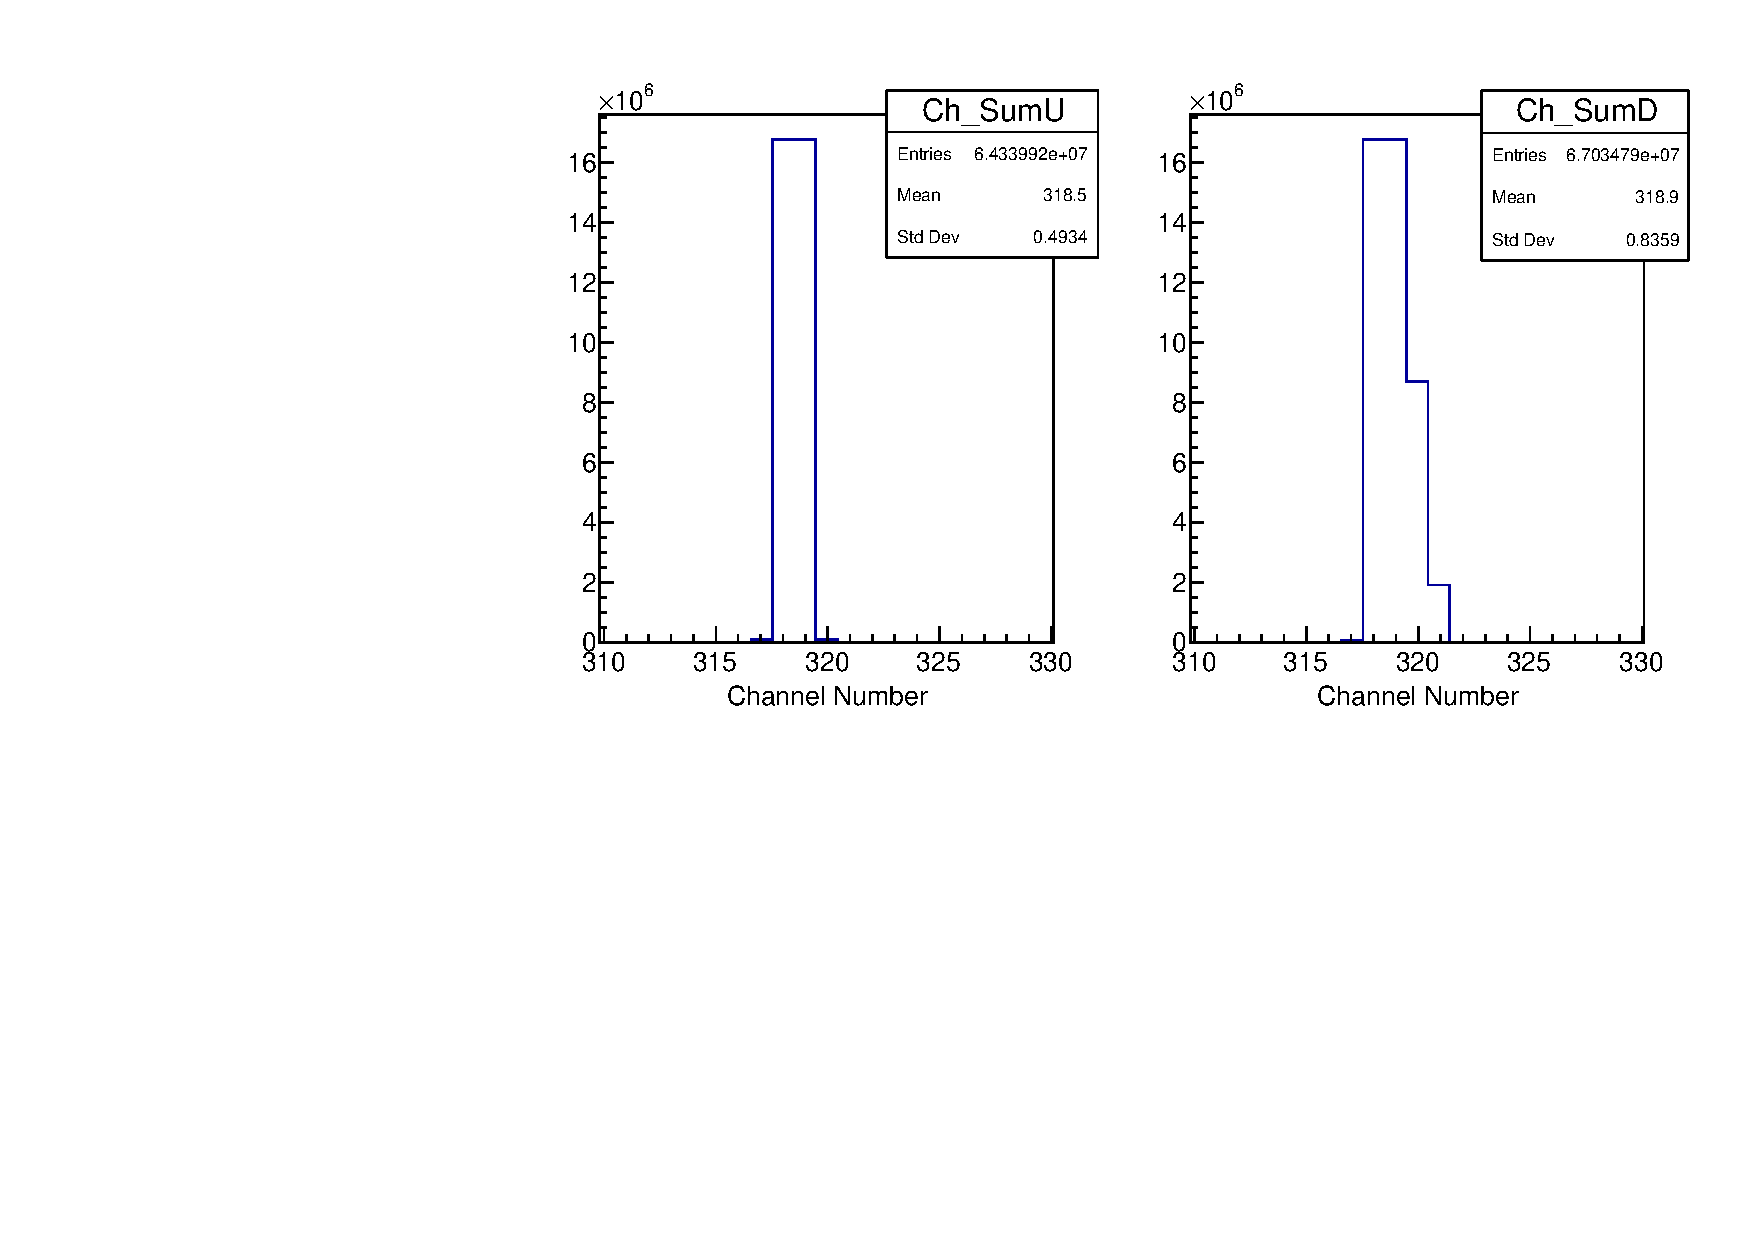
\includegraphics[width=0.7\textwidth, angle=0]{08-Performance/Kuno6mm.pdf}
    \caption{\label{fig:kuno} A plot showing the sum of the channel numbers for the clusters in each spacepoint for the upstream (left) and downstream (right) trackers. Kuno's conjecture that the sum is a constant is observed, with a small variation arising from the way fibre overlap is modelled in the Monte Carlo.}
  \end{figure}

  \begin{figure}[p]
    \centering
    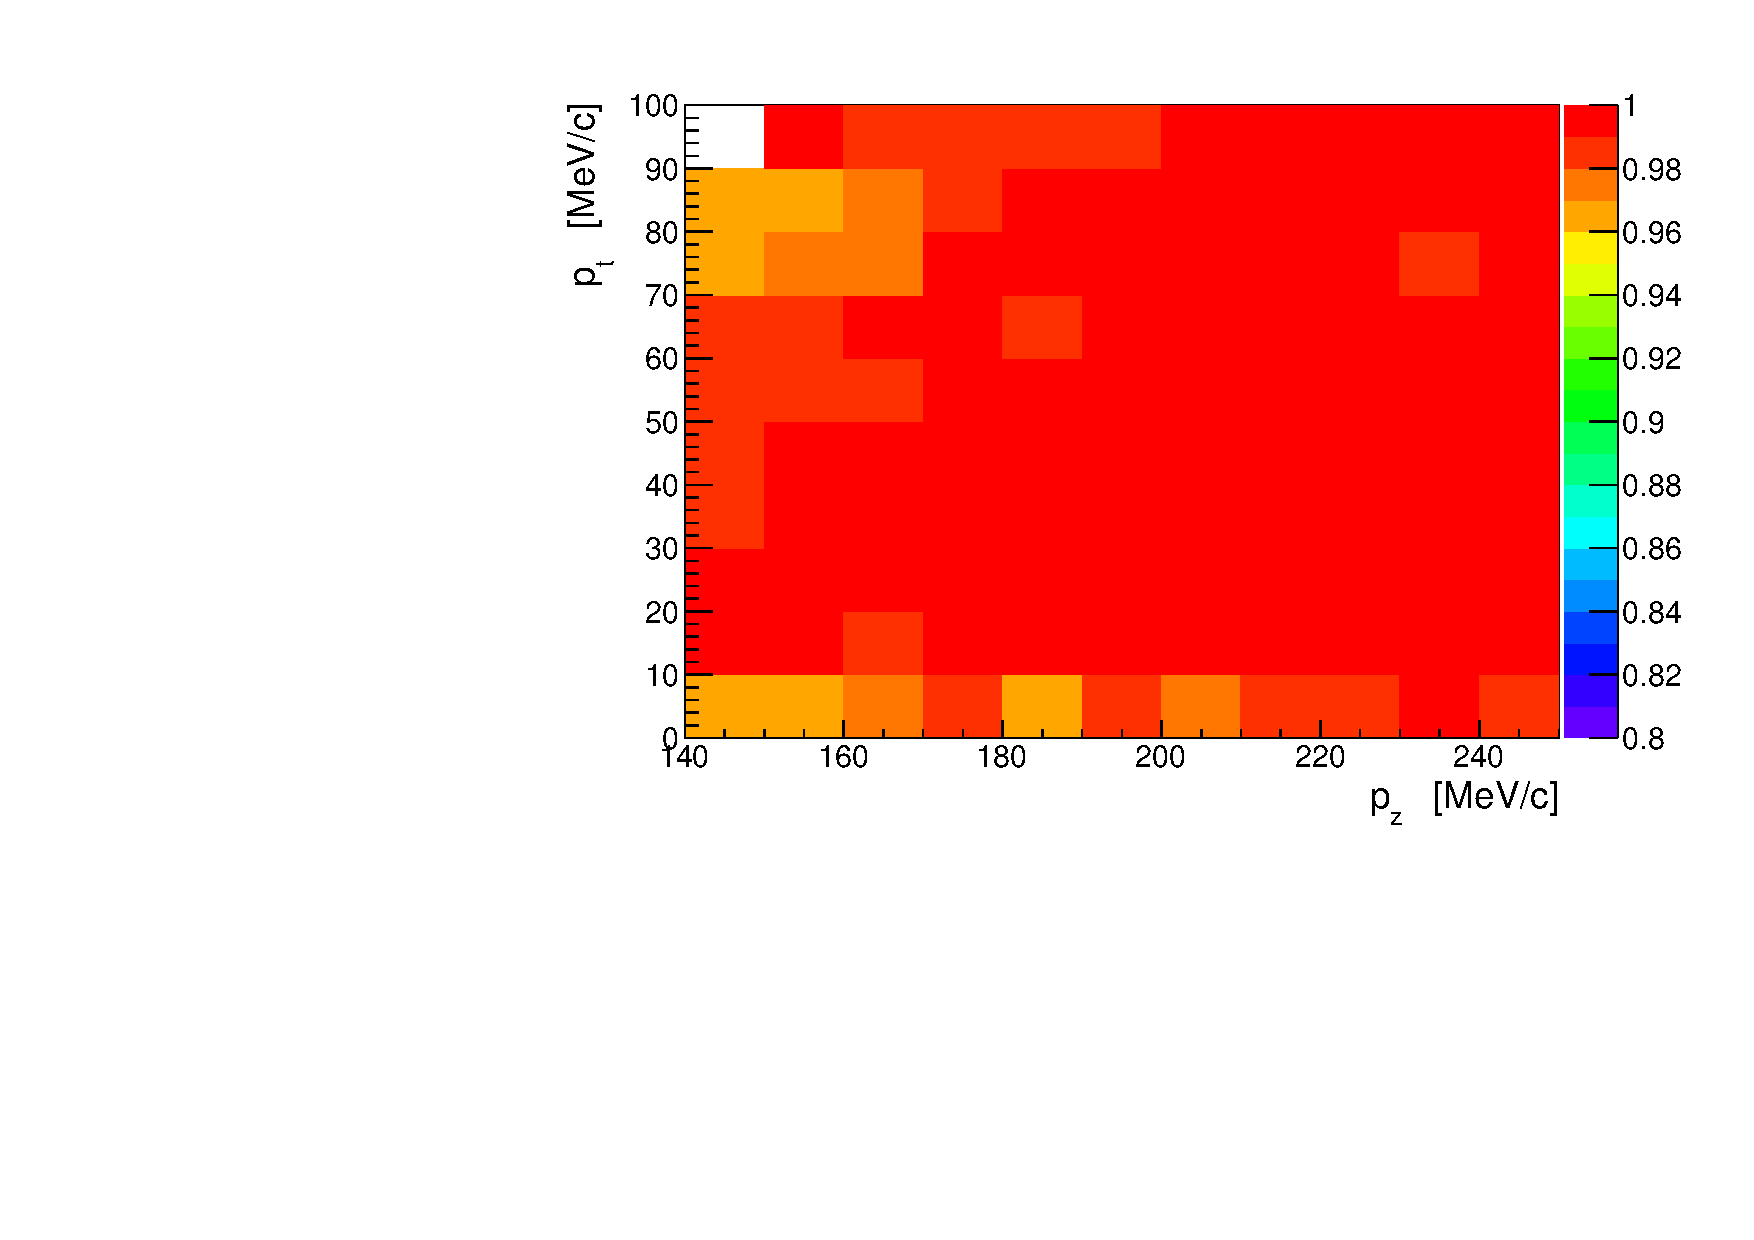
\includegraphics[width=0.495\textwidth, angle=0]{08-Performance/upstream_track_efficiency.pdf}
    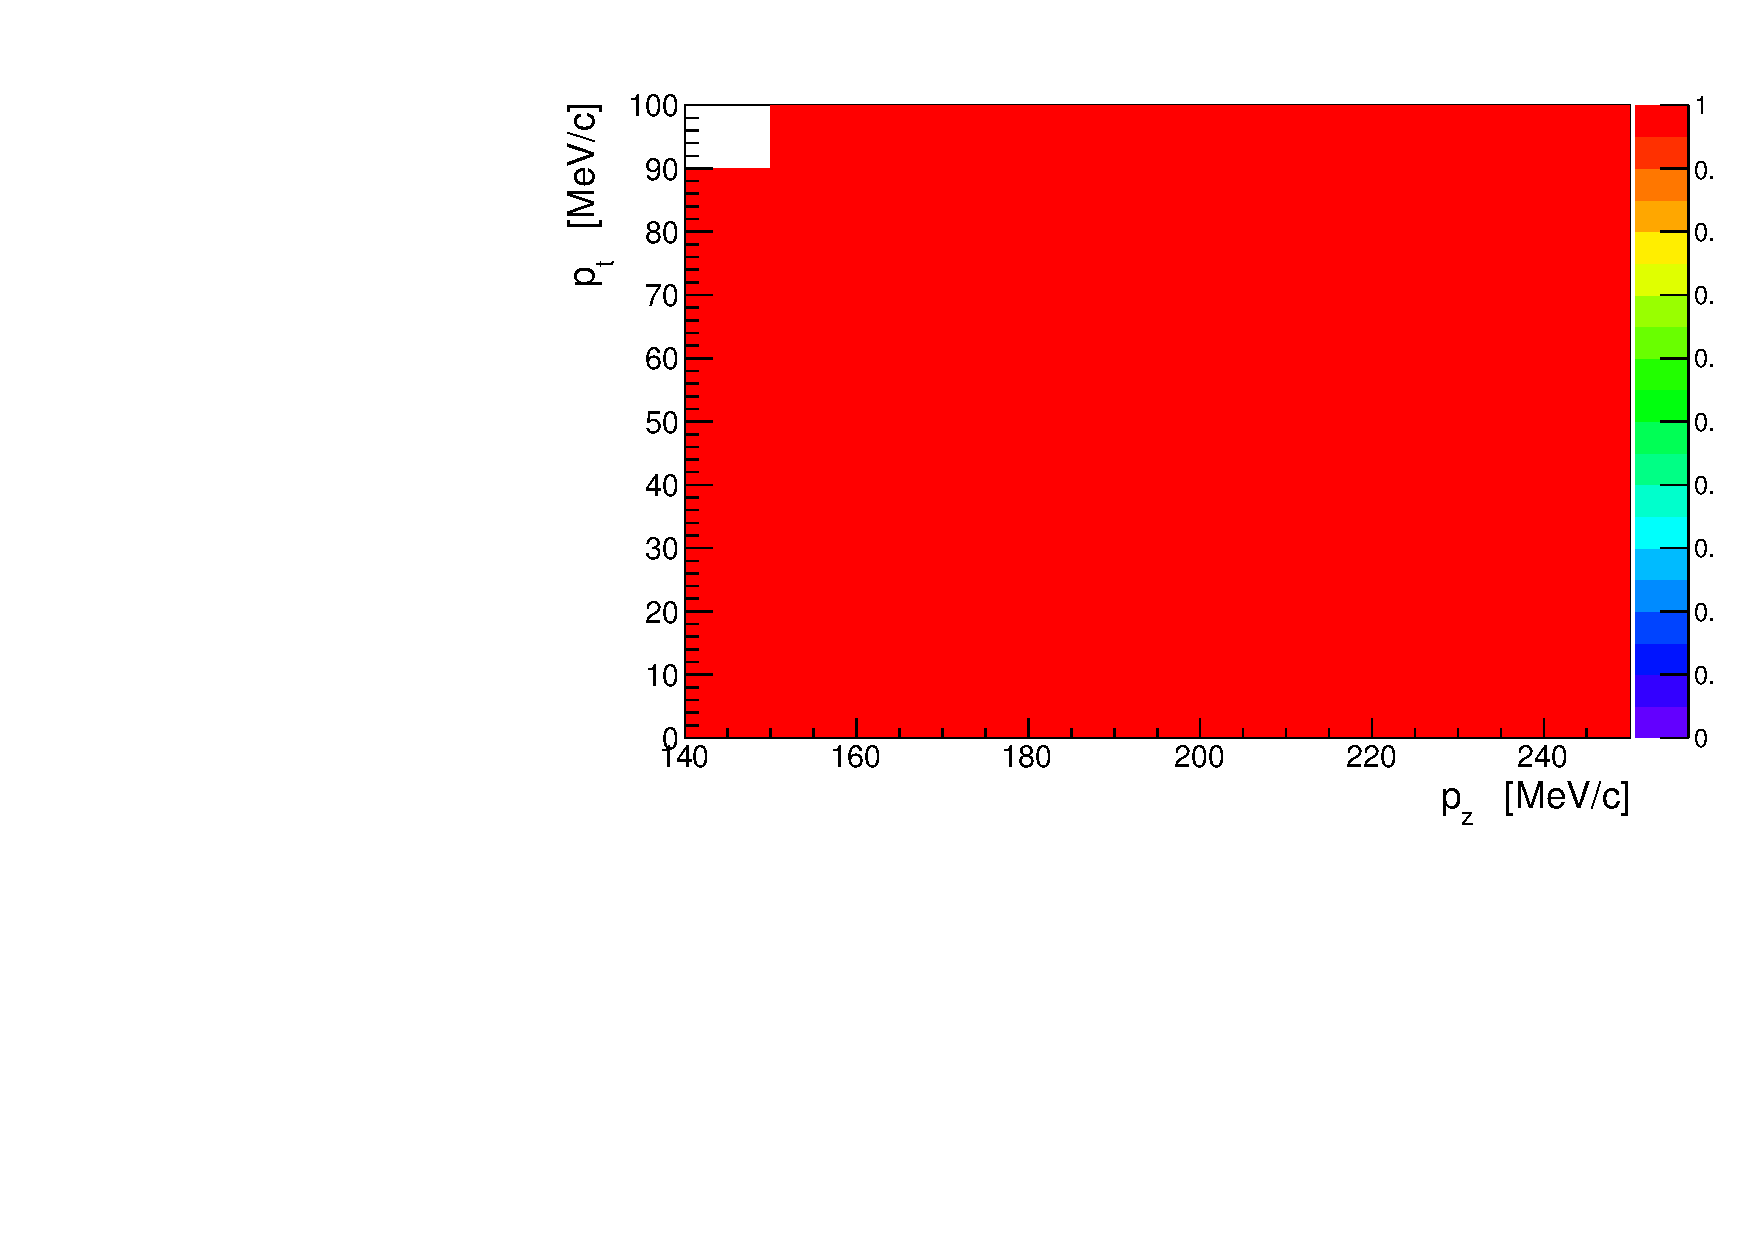
\includegraphics[width=0.495\textwidth, angle=0]{08-Performance/downstream_track_efficiency.pdf}\\
    \caption{\label{fig:track_efficiency} The efficiency of reconstructing tracks in the upstream (left) and downstream (right) trackers as a function of the simulated longitudinal and transverse momentum. The white area in the top left of the plot indicates events which fall outside of the $p_t/p_z$ ratio cut.}
  \end{figure}

%   \begin{figure}[p]
%     \centering
%     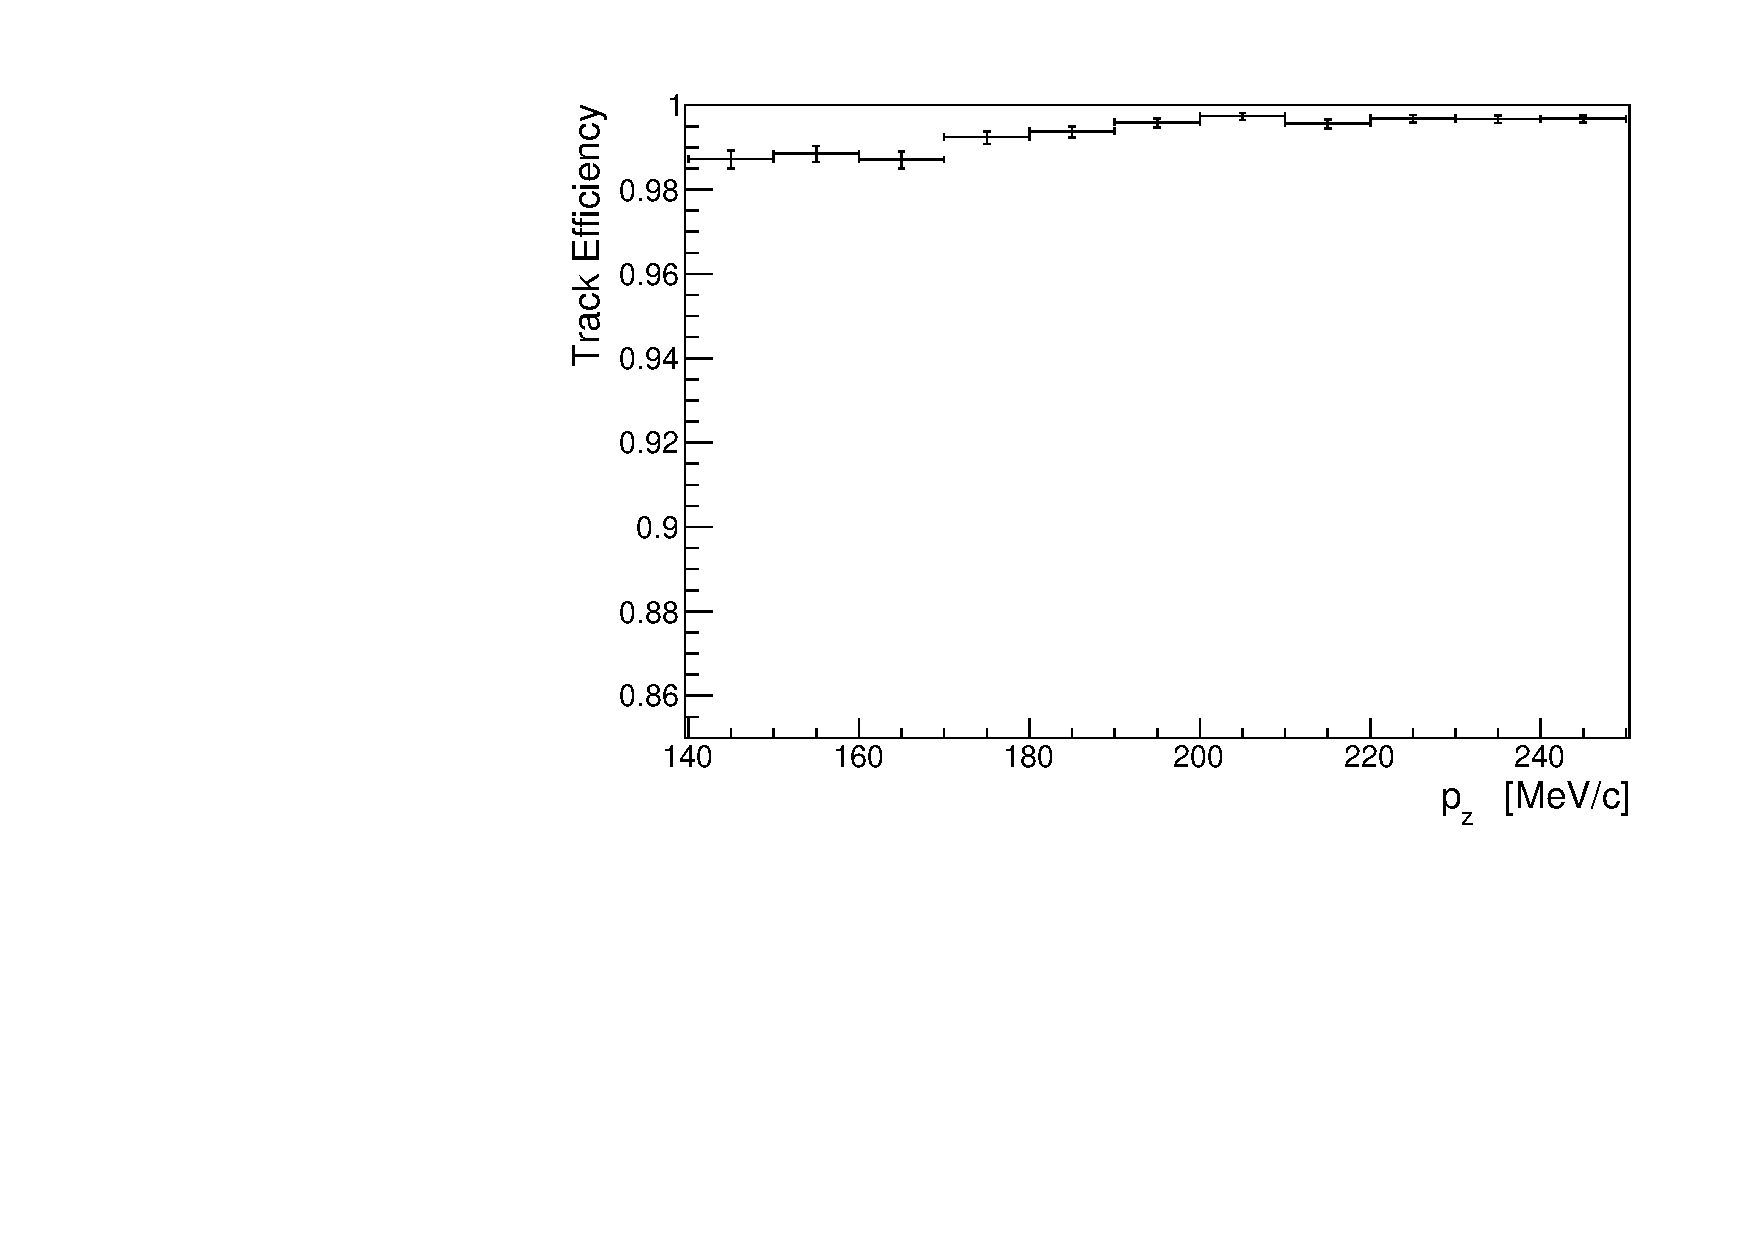
\includegraphics[width=0.45\textwidth, angle=0]{08-Performance/upstream_pz_track_efficiency.pdf}
%     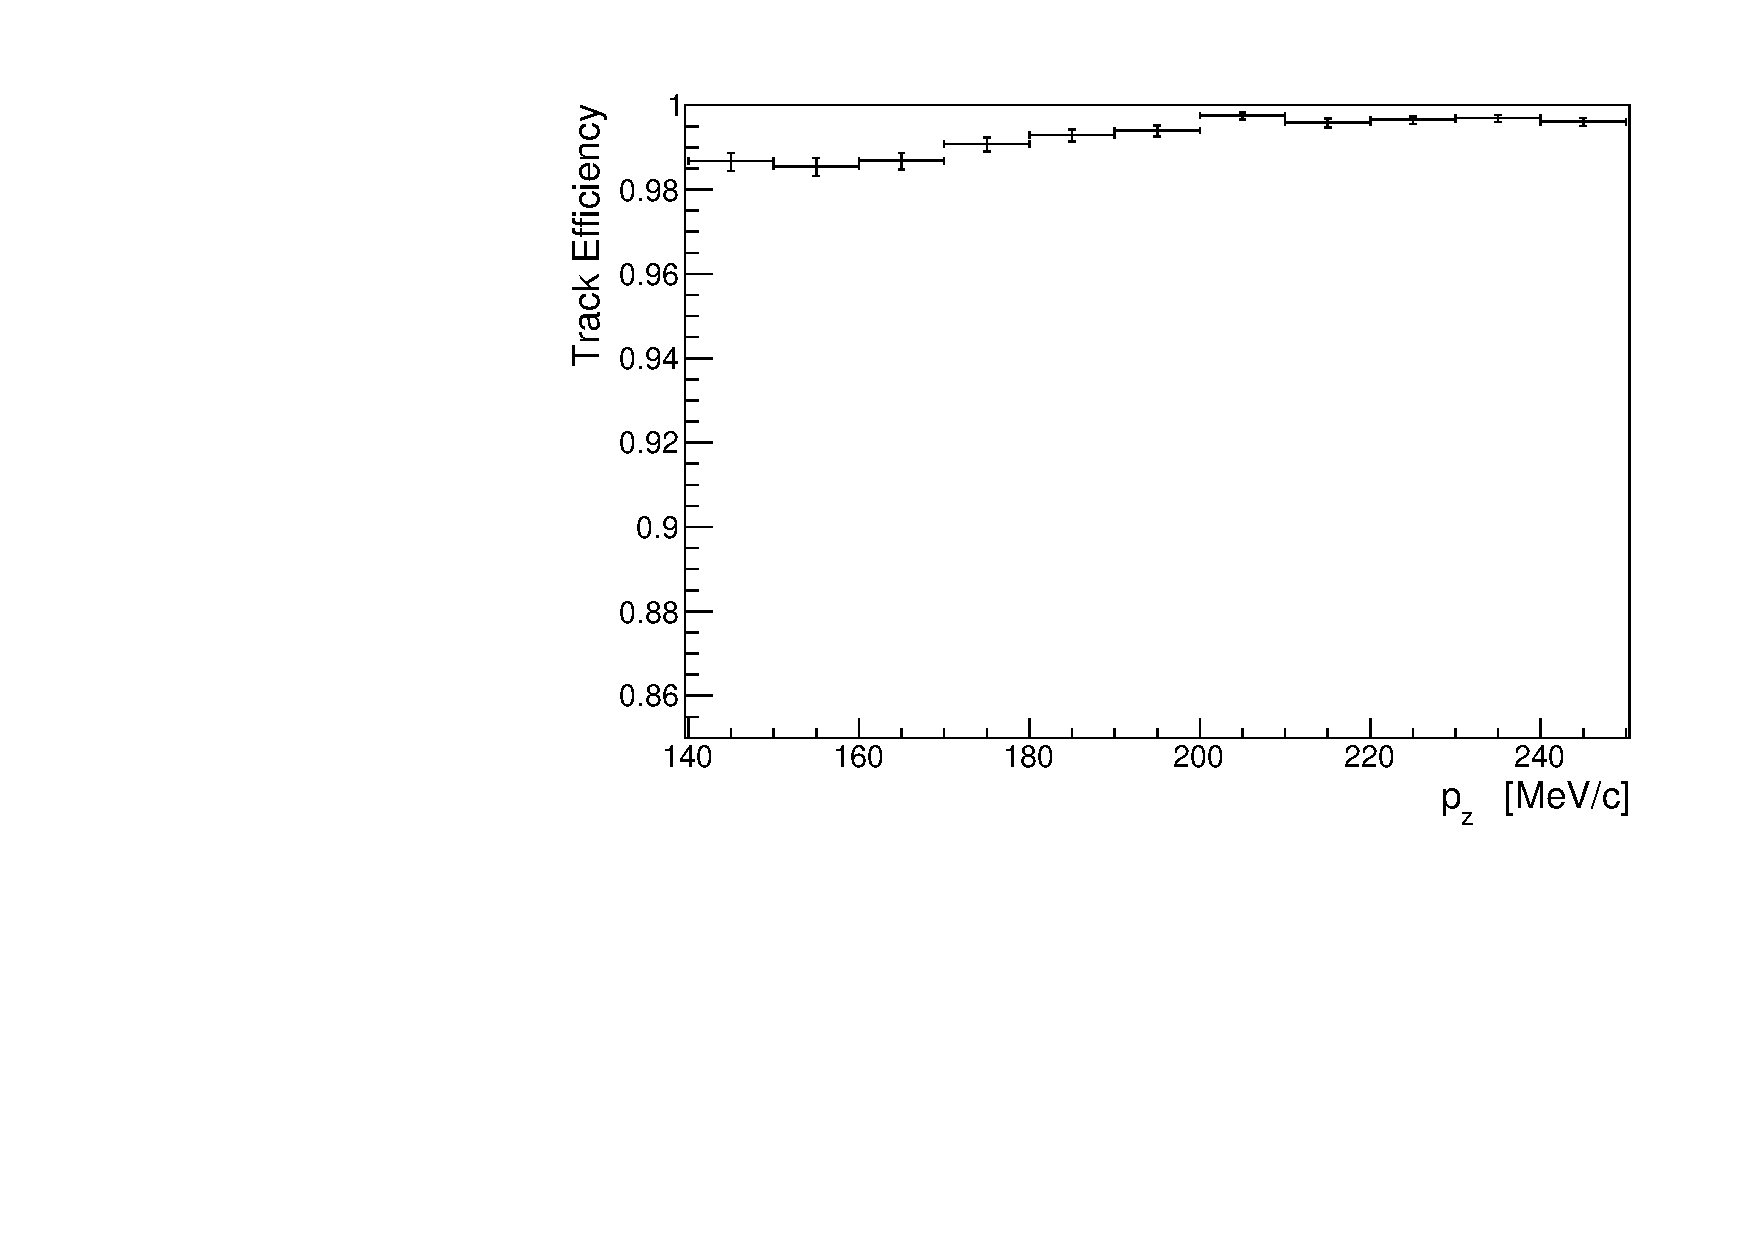
\includegraphics[width=0.45\textwidth, angle=0]{08-Performance/downstream_pz_track_efficiency.pdf}\\
%     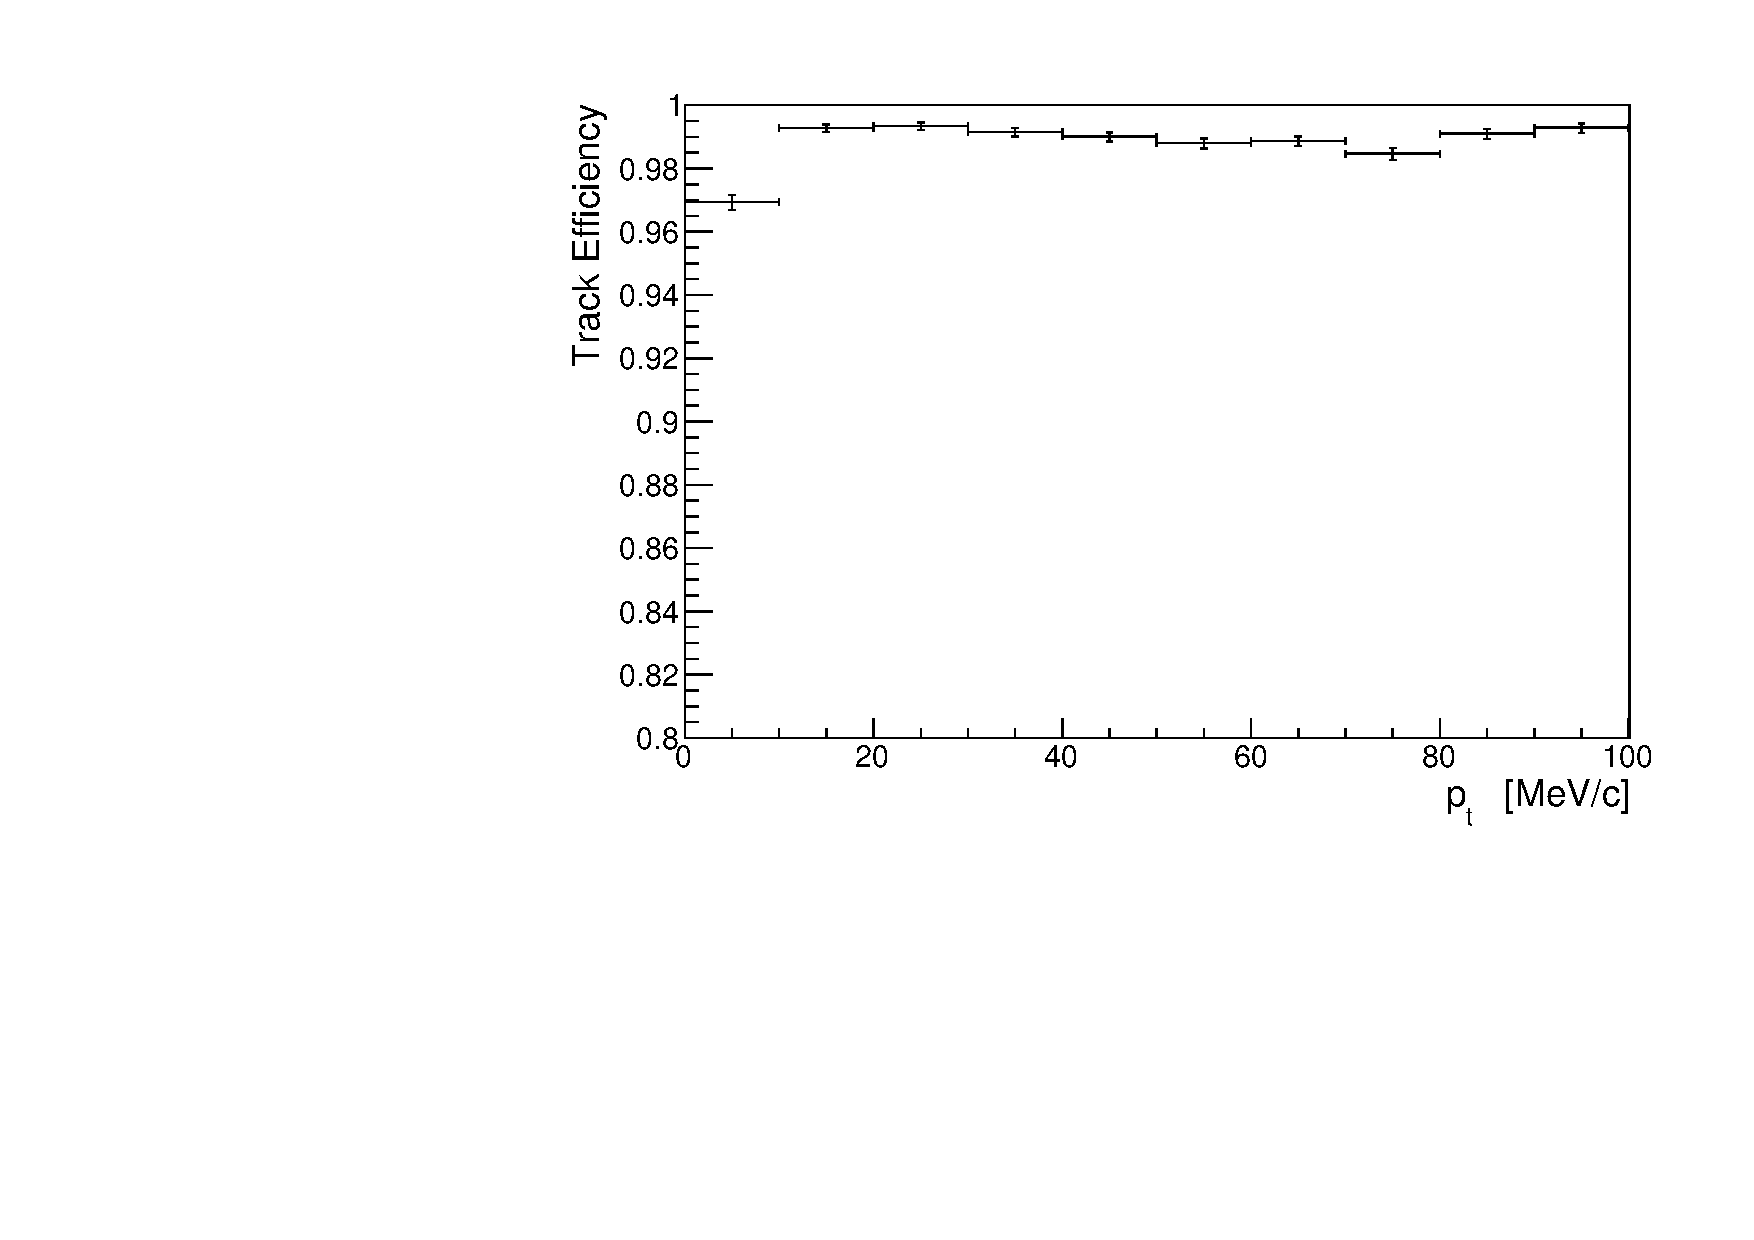
\includegraphics[width=0.45\textwidth, angle=0]{08-Performance/upstream_pt_track_efficiency.pdf}
%     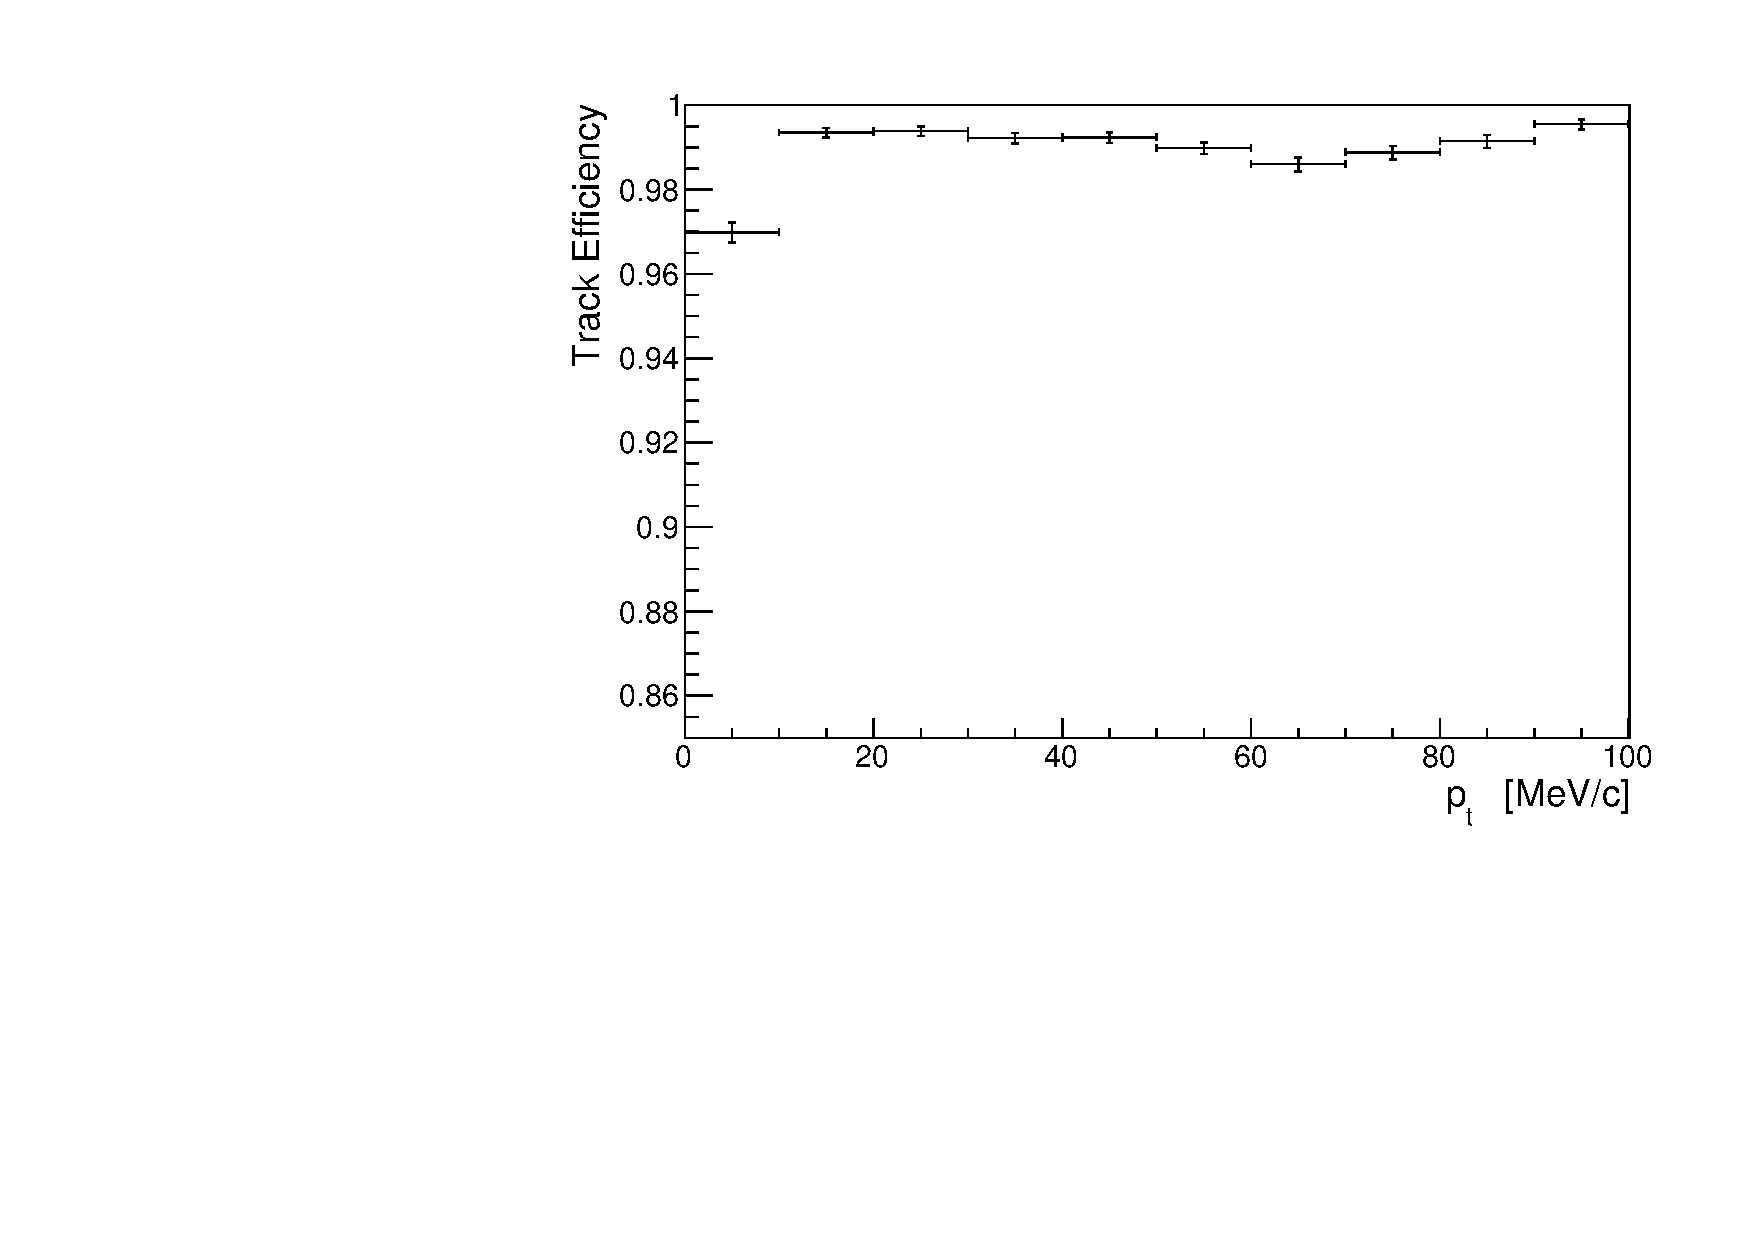
\includegraphics[width=0.45\textwidth, angle=0]{08-Performance/downstream_pt_track_efficiency.pdf}
%     \caption{\label{fig:track_efficiency} The efficiency of reconstructing tracks in the upstream (left) and downstream (right) trackers as a function of the simulated longitudinal (top) and transverse (bottom) momentum.}
%   \end{figure}
  
%   \begin{figure}[p]
%     \centering
%     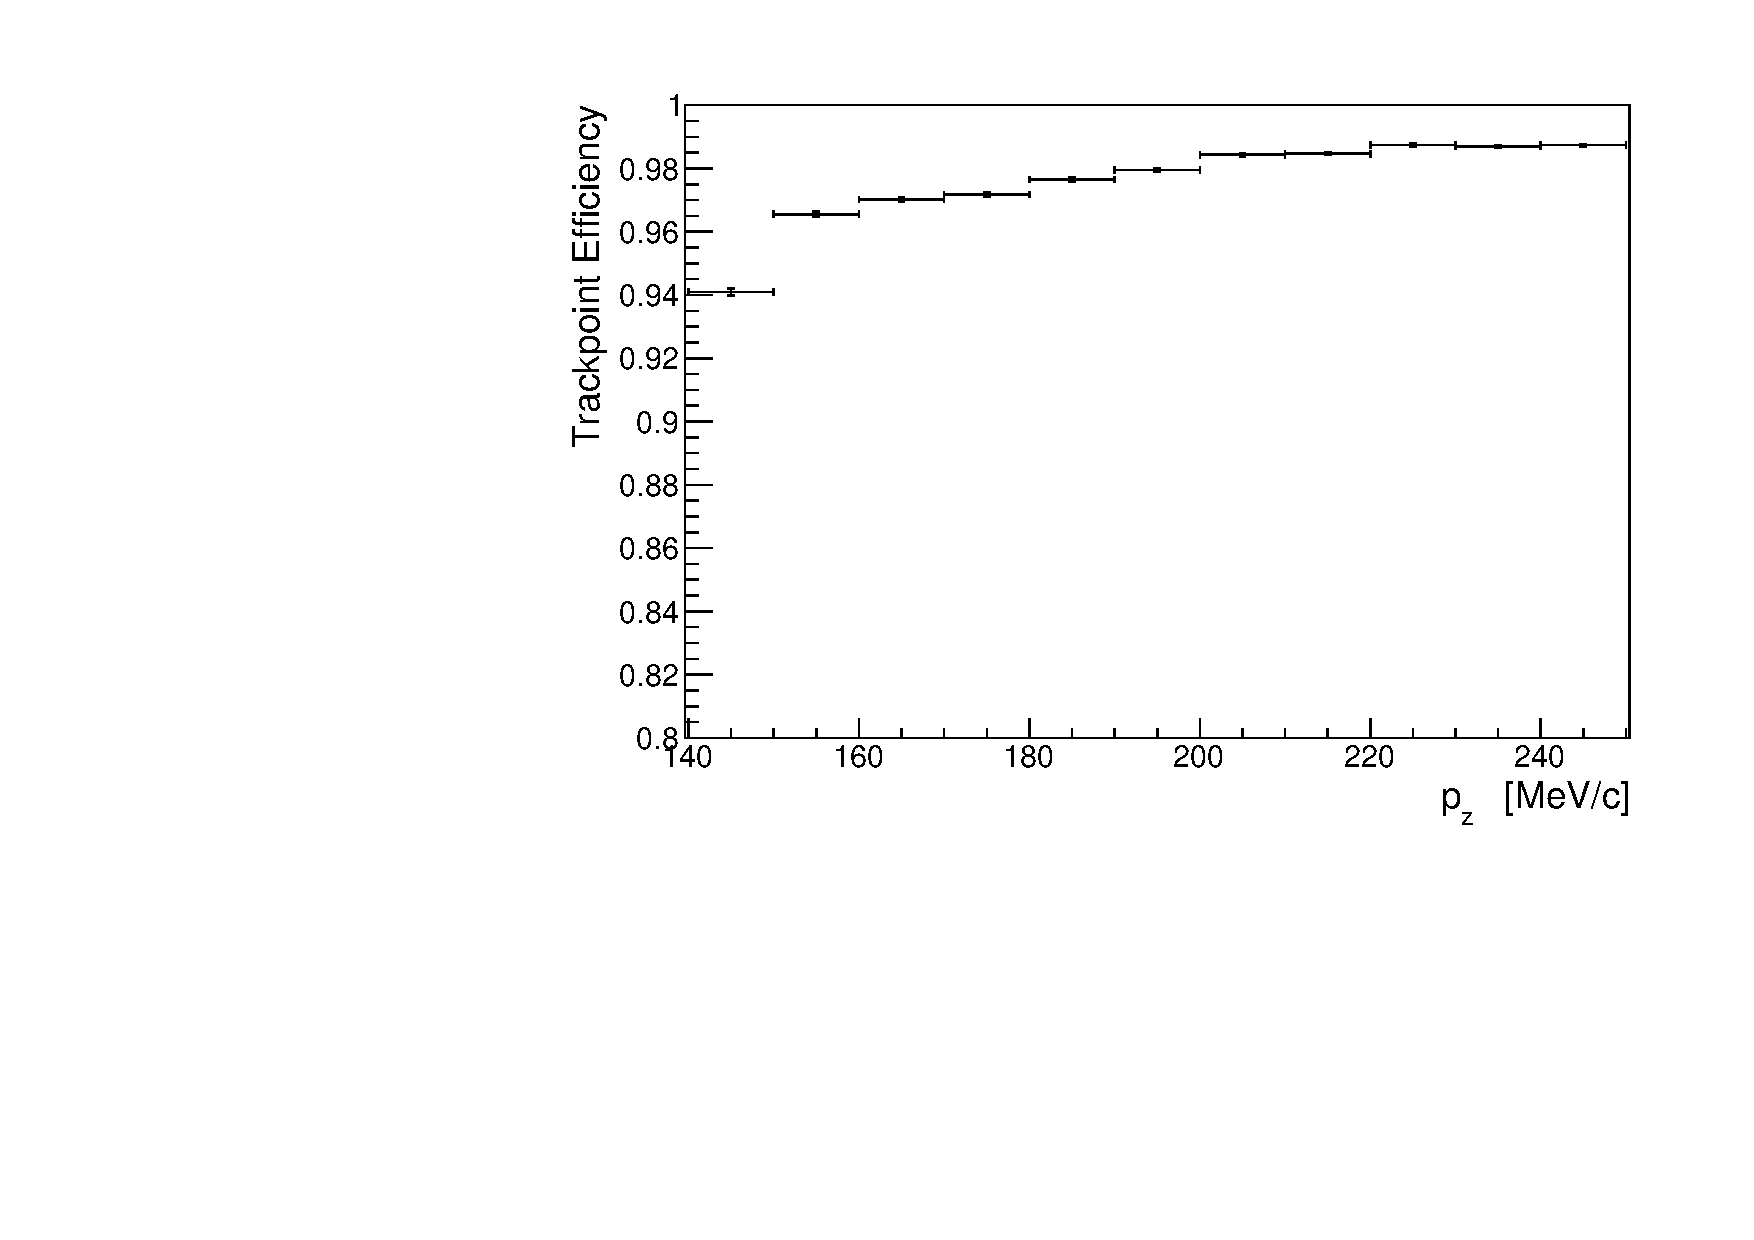
\includegraphics[width=0.45\textwidth, angle=0]{08-Performance/upstream_pz_tp_efficiency.pdf}
%     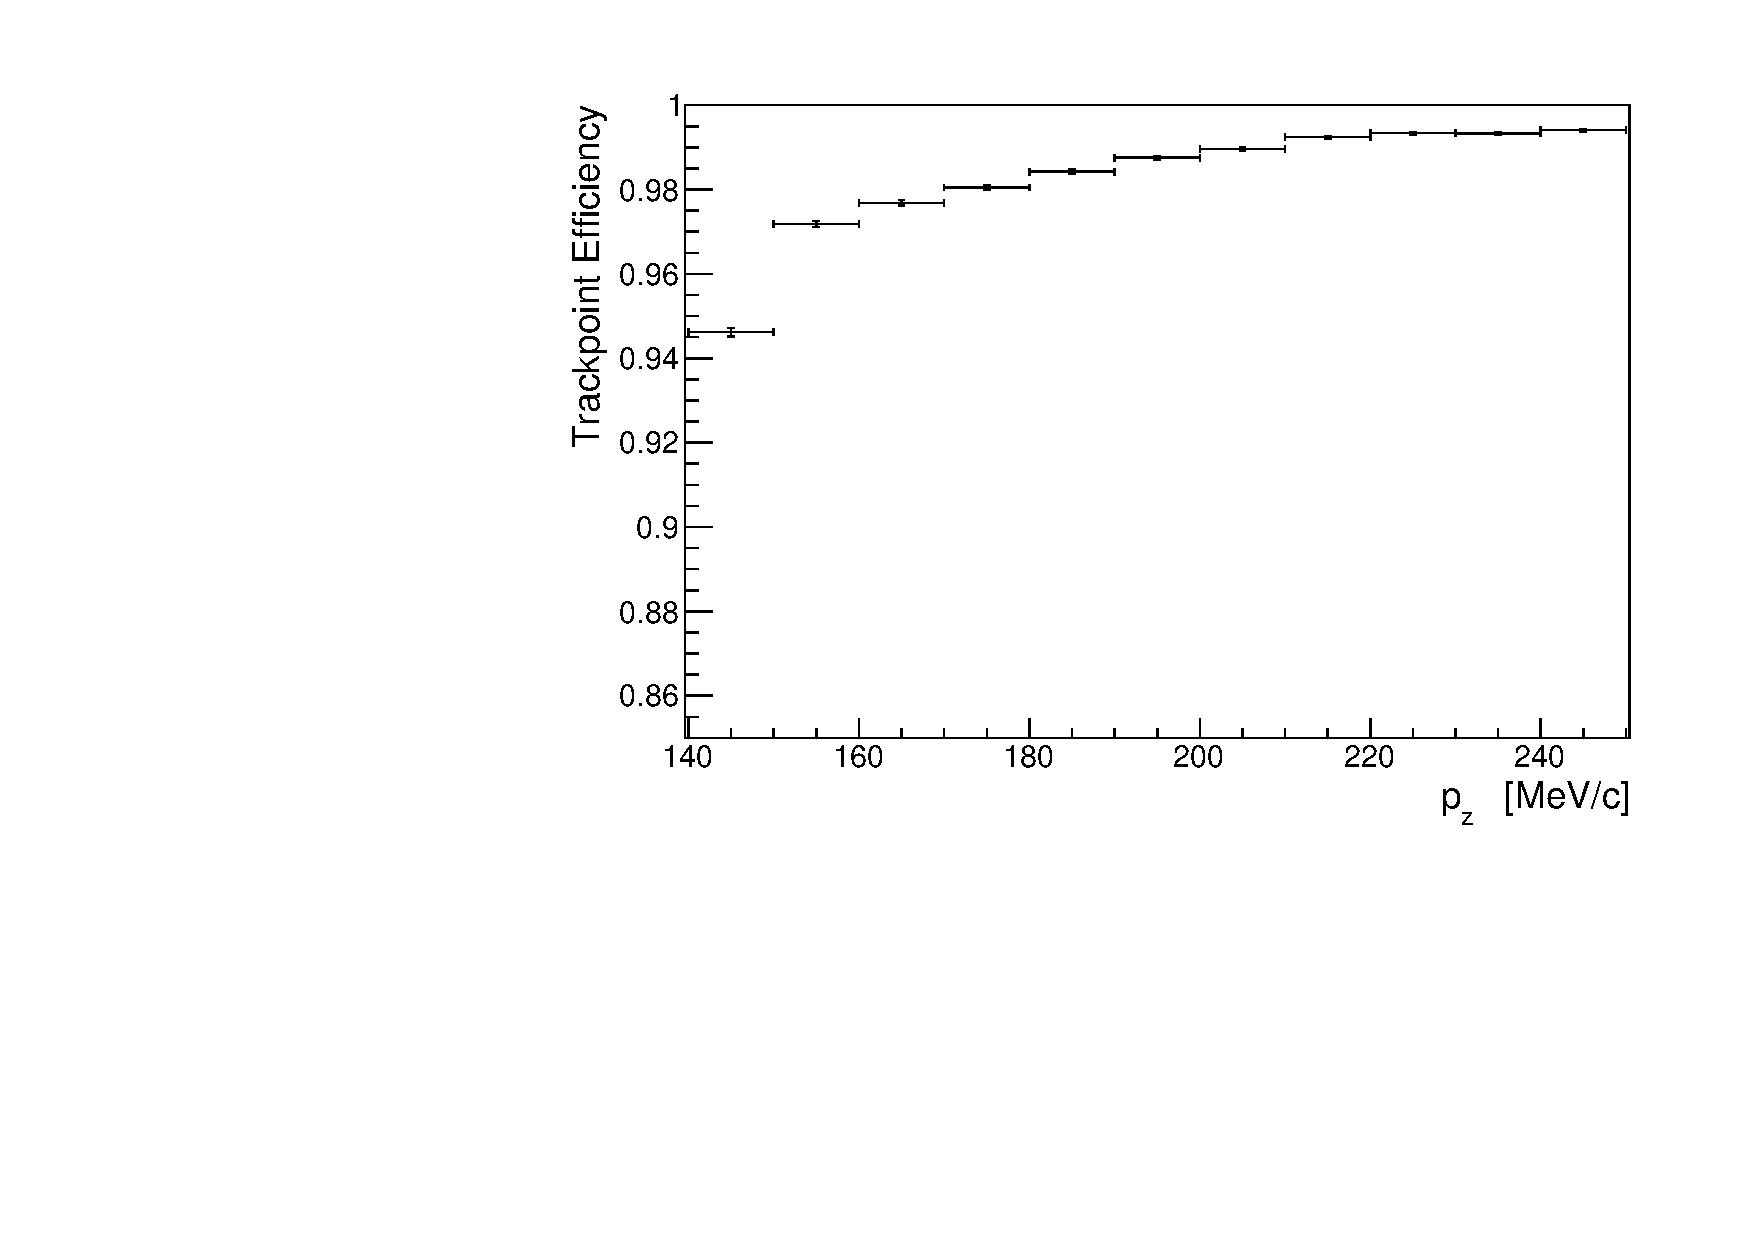
\includegraphics[width=0.45\textwidth, angle=0]{08-Performance/downstream_pz_tp_efficiency.pdf}\\
%     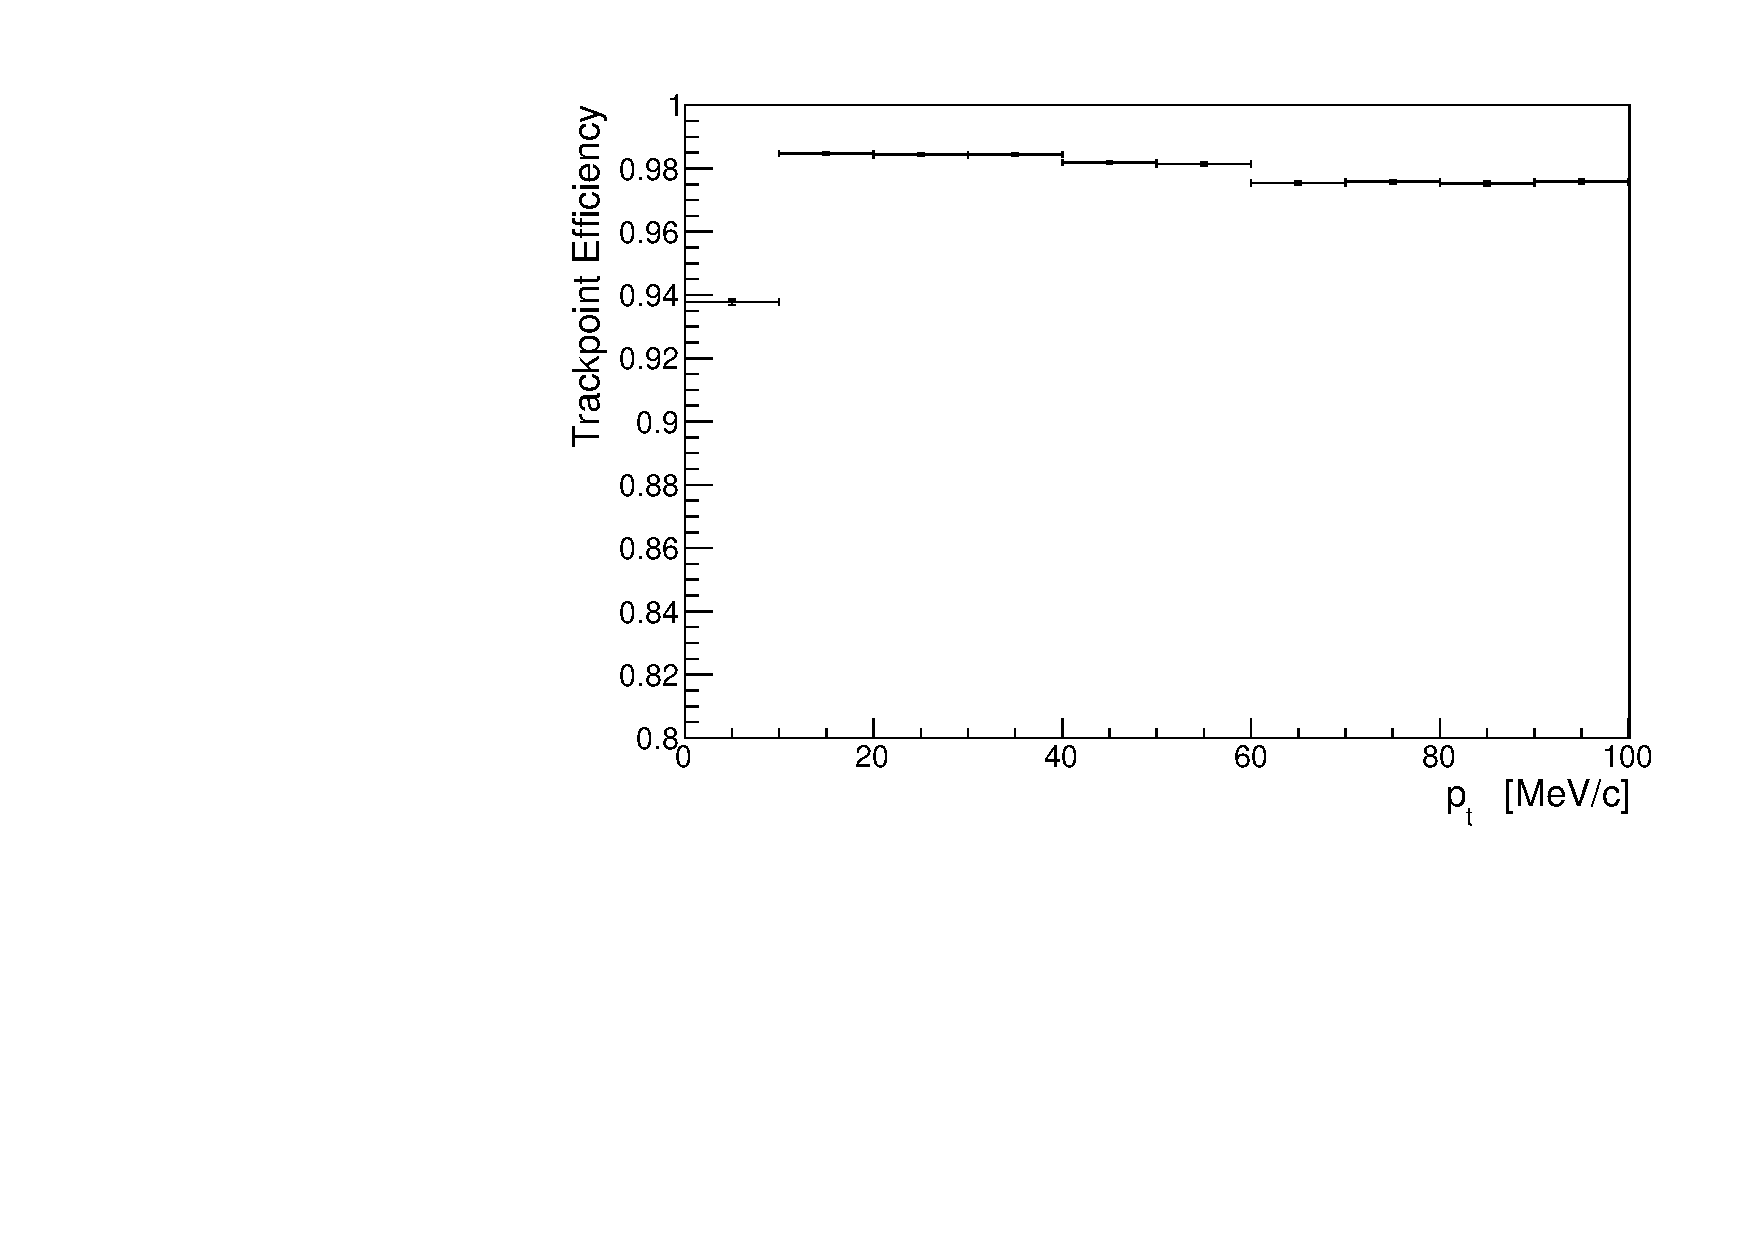
\includegraphics[width=0.45\textwidth, angle=0]{08-Performance/upstream_pt_tp_efficiency.pdf}
%     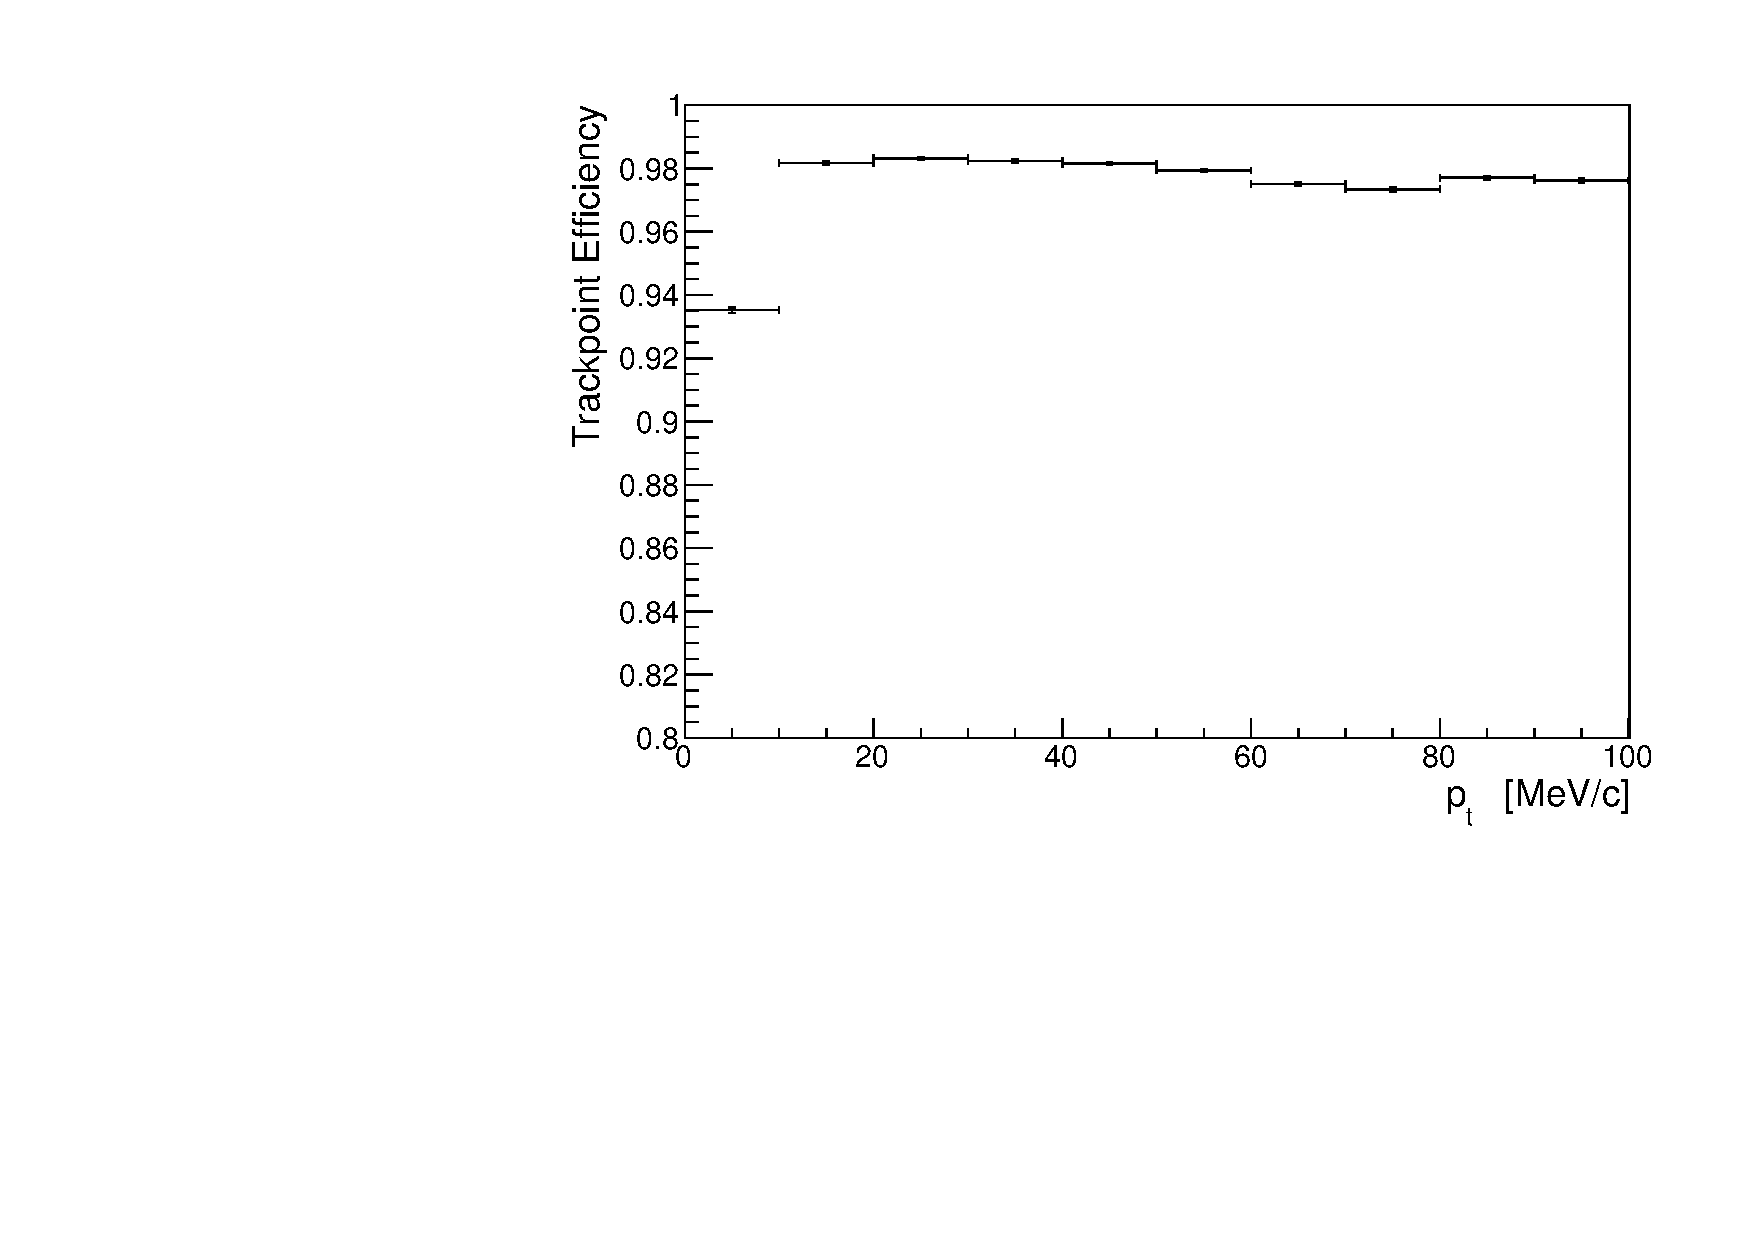
\includegraphics[width=0.45\textwidth, angle=0]{08-Performance/downstream_pt_tp_efficiency.pdf}
%     \caption{\label{fig:tp_efficiency} The efficiency of reconstructing trackpoints in the upstream (left) and downstream (right) trackers as a function of the simulated longitudinal (top) and transverse (bottom) momentum.}
%   \end{figure}
  
  \begin{figure}[p]
   \centering
    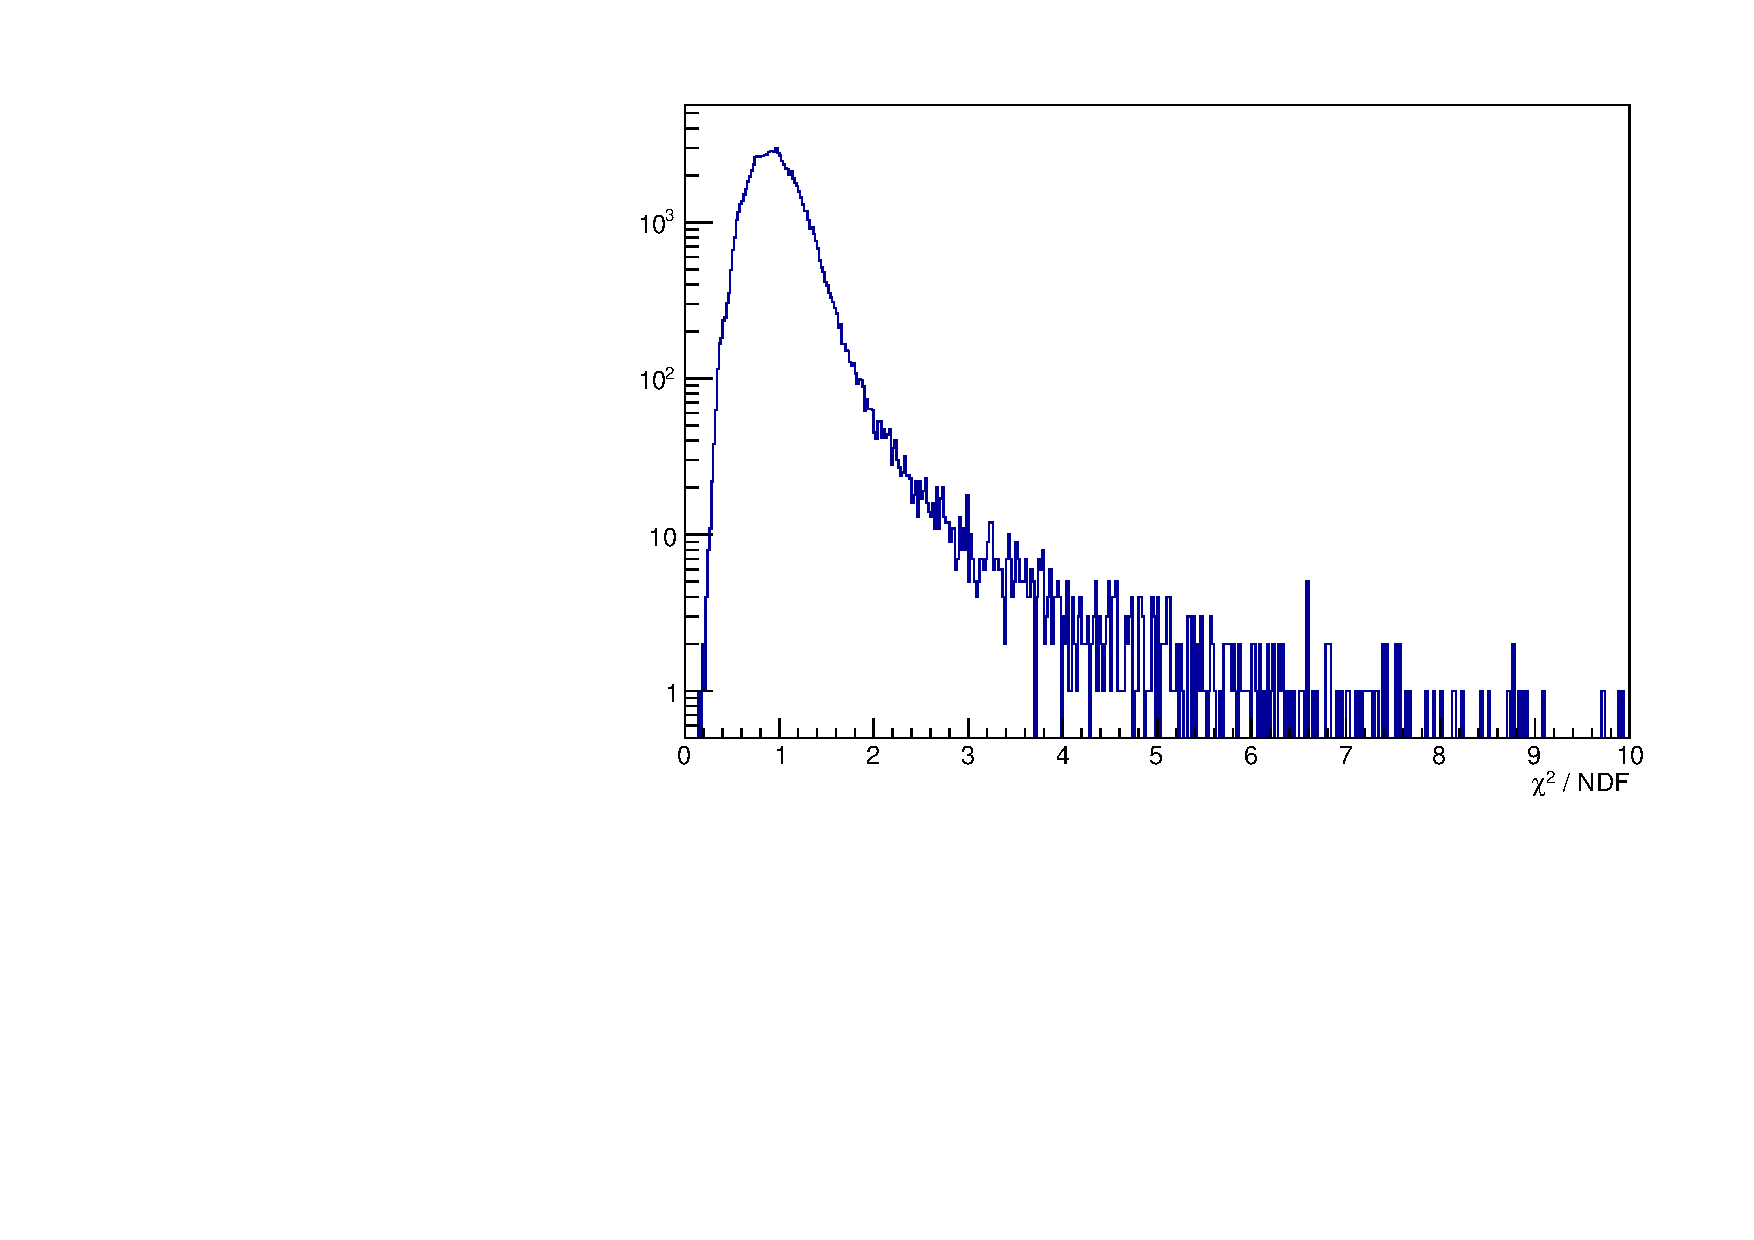
\includegraphics[width=0.49\textwidth, angle=0]{08-Performance/chi_squared_ndf_up.pdf}
    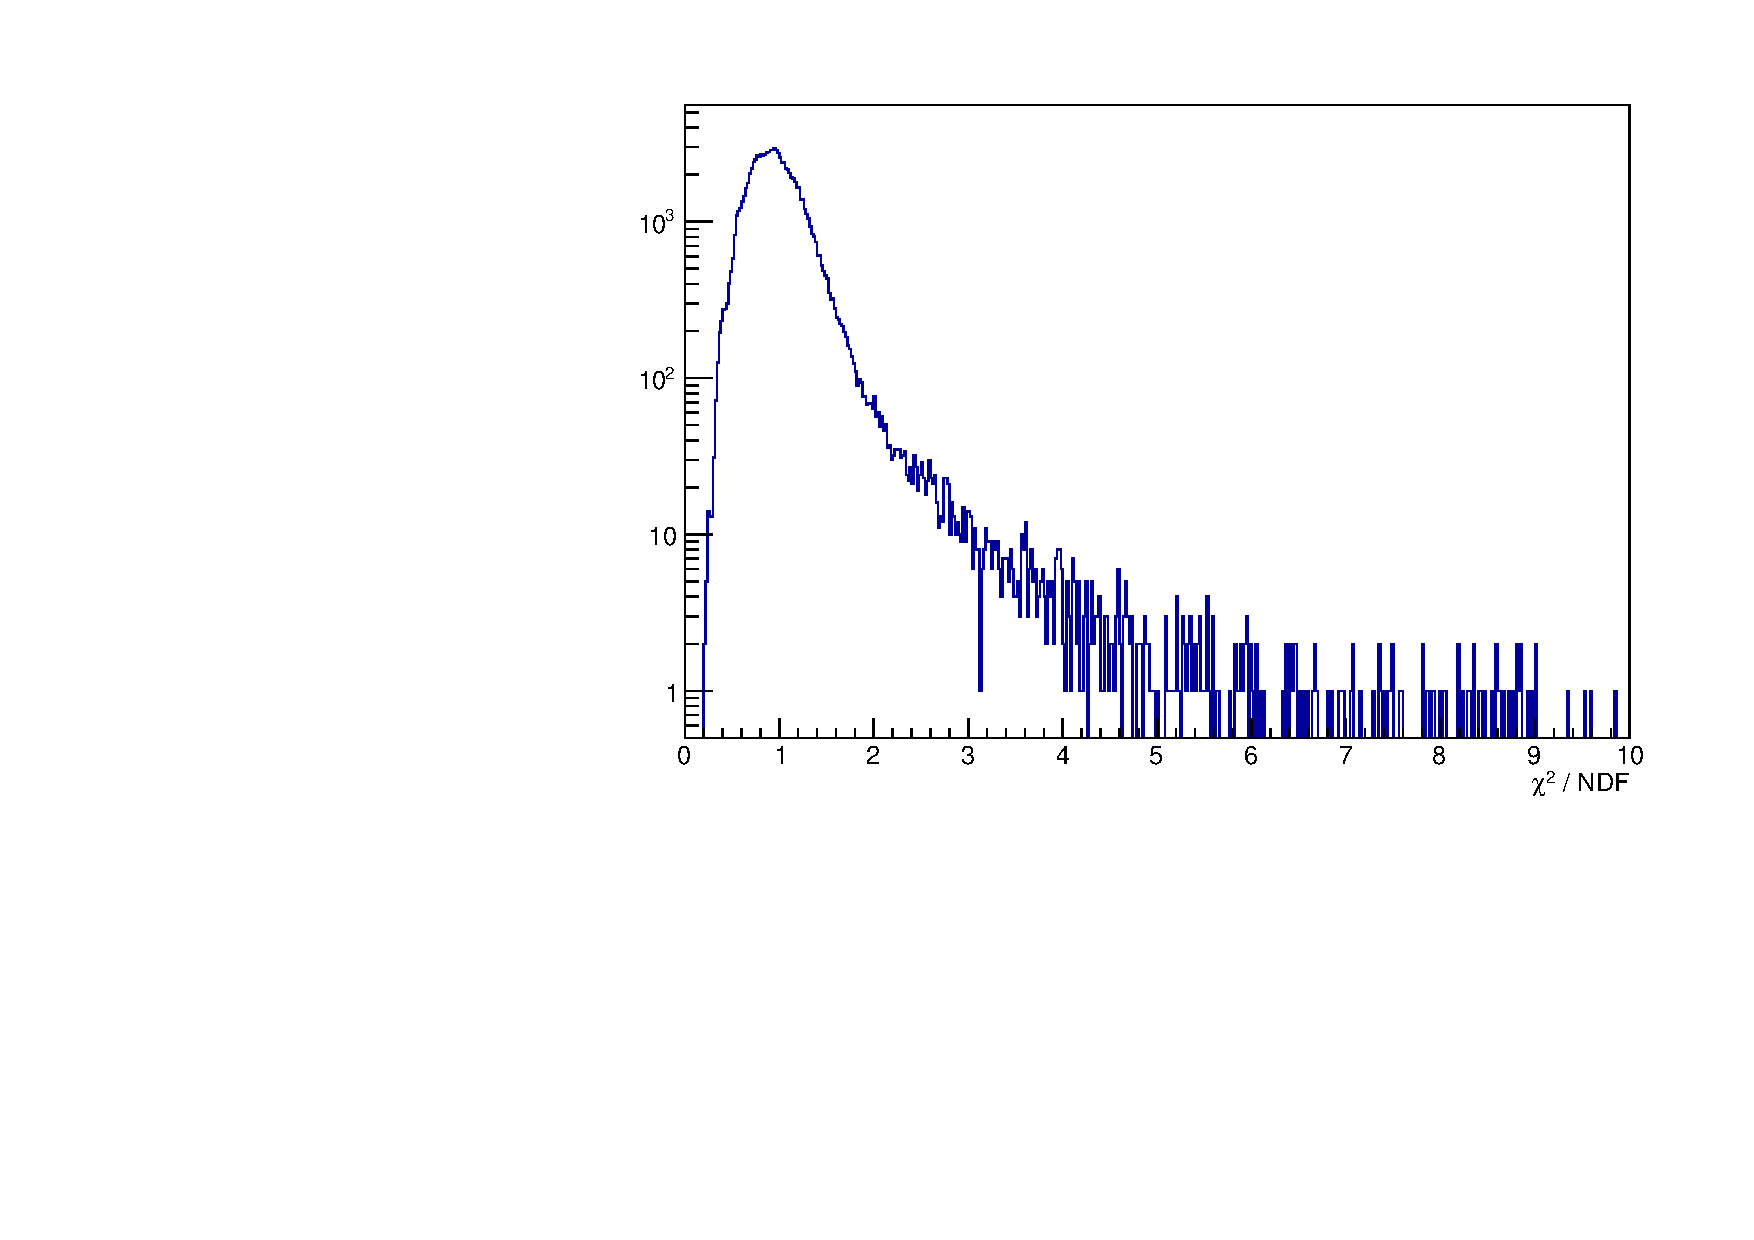
\includegraphics[width=0.49\textwidth, angle=0]{08-Performance/chi_squared_ndf_down.pdf}
   \caption{\label{fig:track_chisq} The $\chi^2$ per degree of freedom in the upstream (left) and downstream (right) trackers.}
  \end{figure}
  
  \begin{figure}[p]
    \begin{center}
      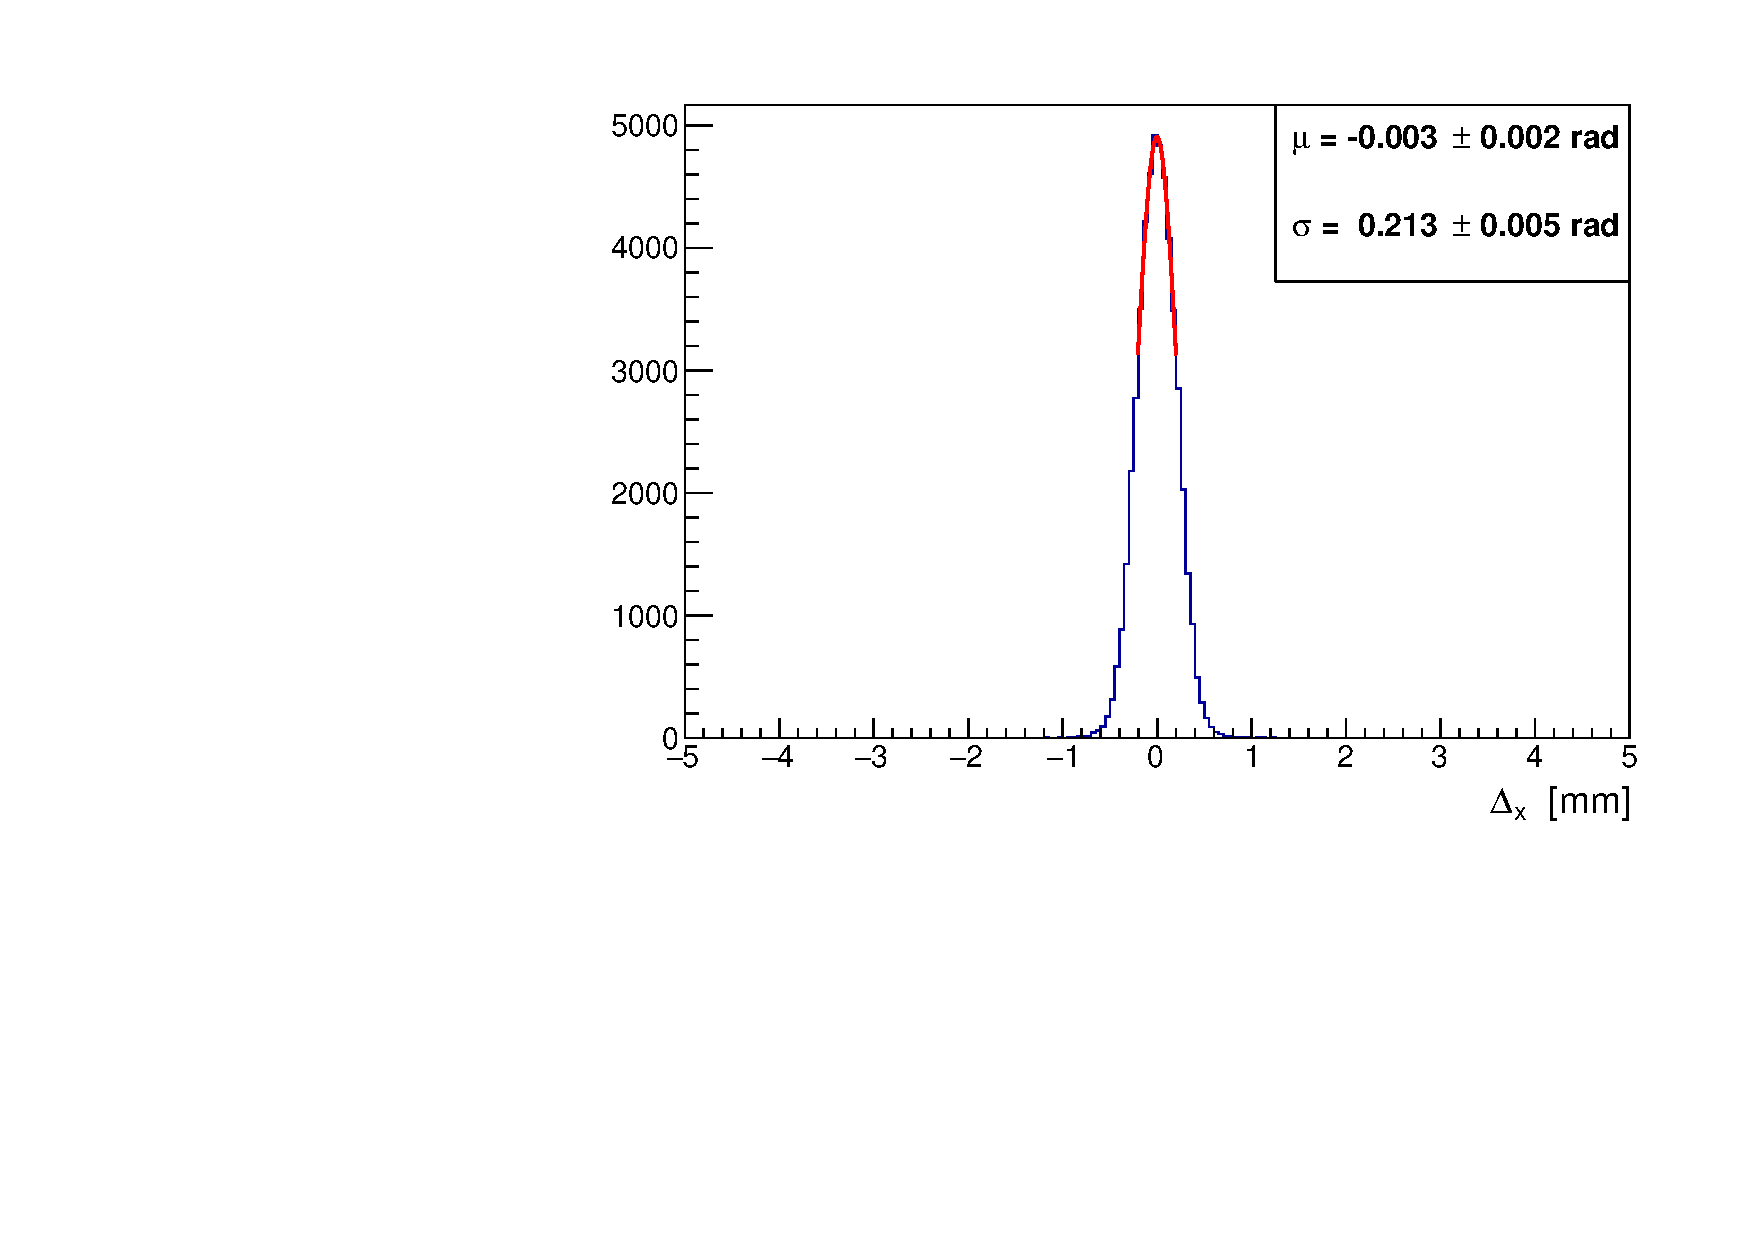
\includegraphics[width=0.49\textwidth, angle=0]{08-Performance/upstream_x_residual.pdf}
      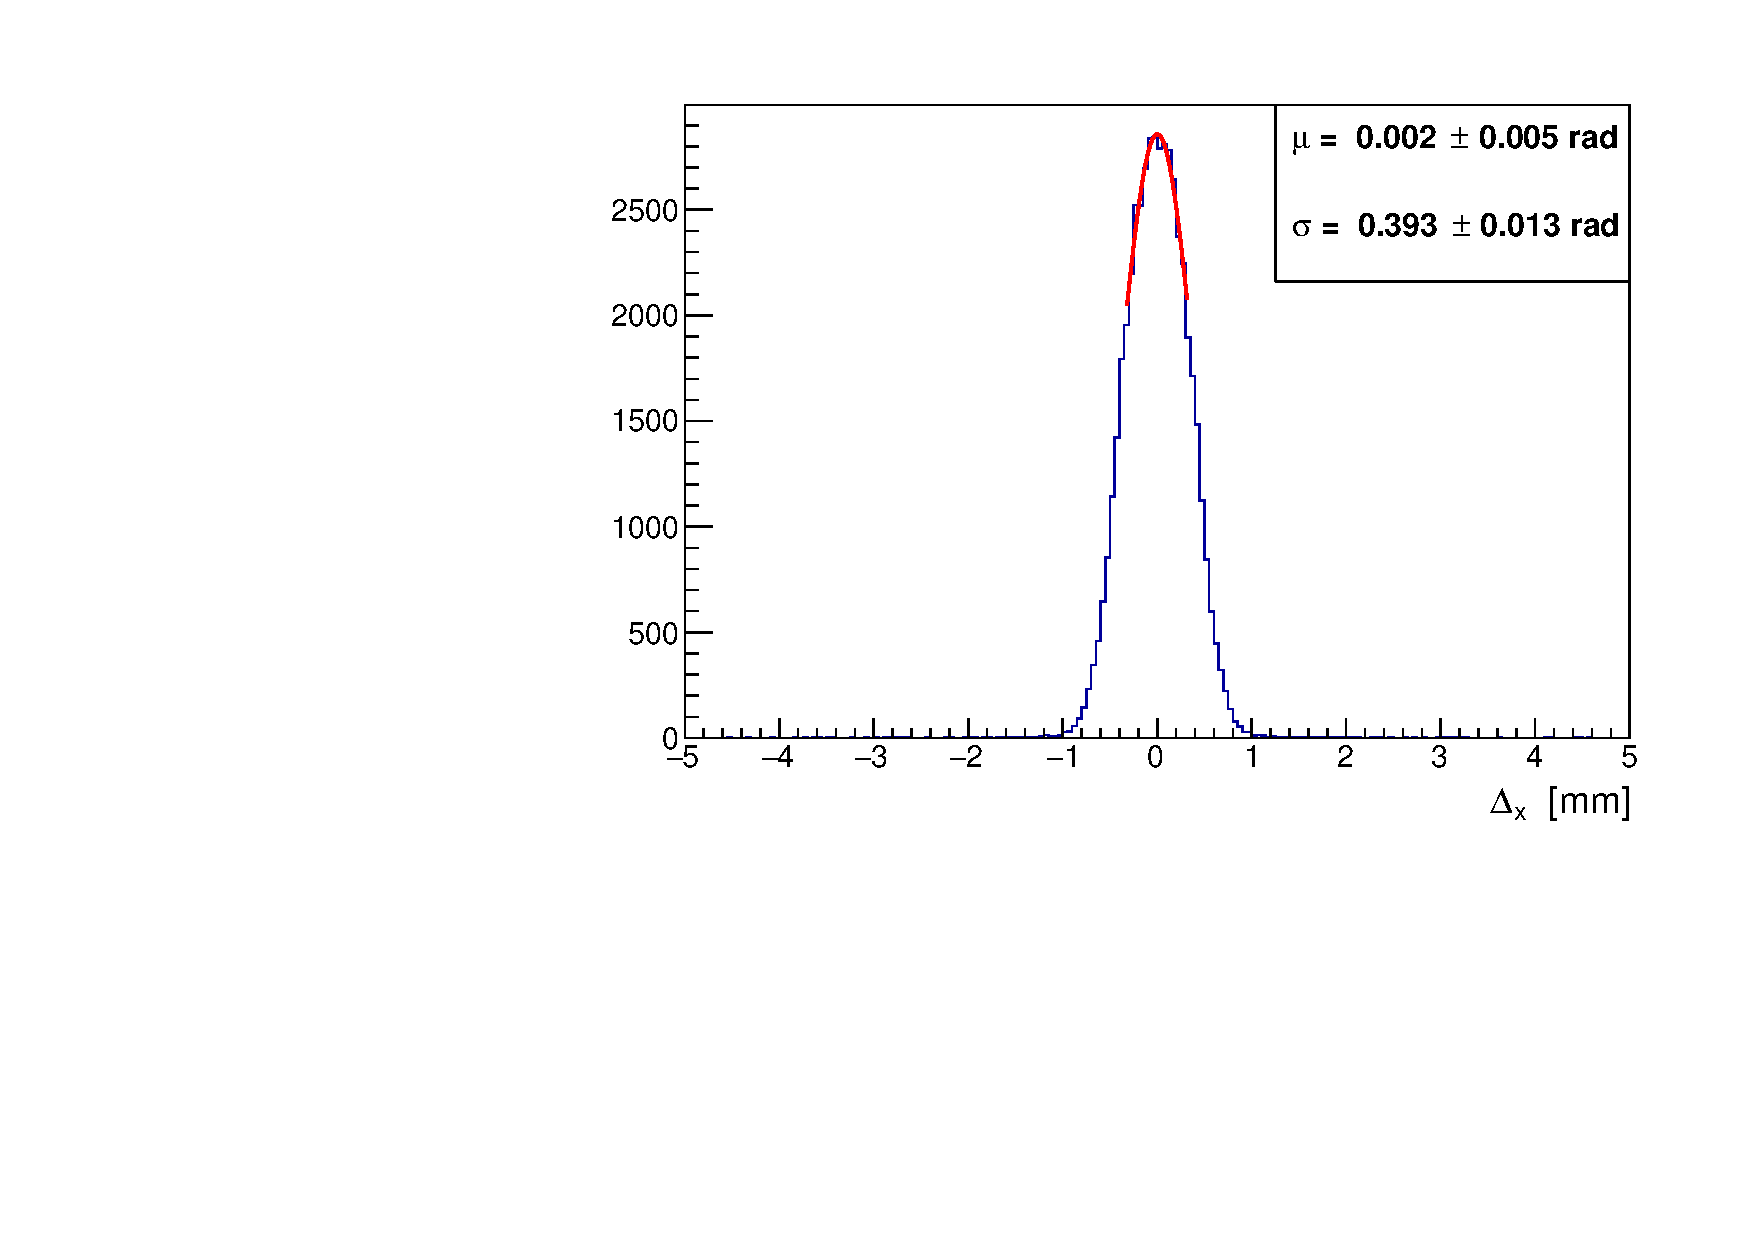
\includegraphics[width=0.49\textwidth, angle=0]{08-Performance/downstream_x_residual.pdf}
      \caption{\label{fig:XResidKalman} The $x$ residuals of the upstream (left) and downstream (right) trackers.}
    \end{center}
  \end{figure}
  
    \begin{figure}[p]
    \begin{center}
      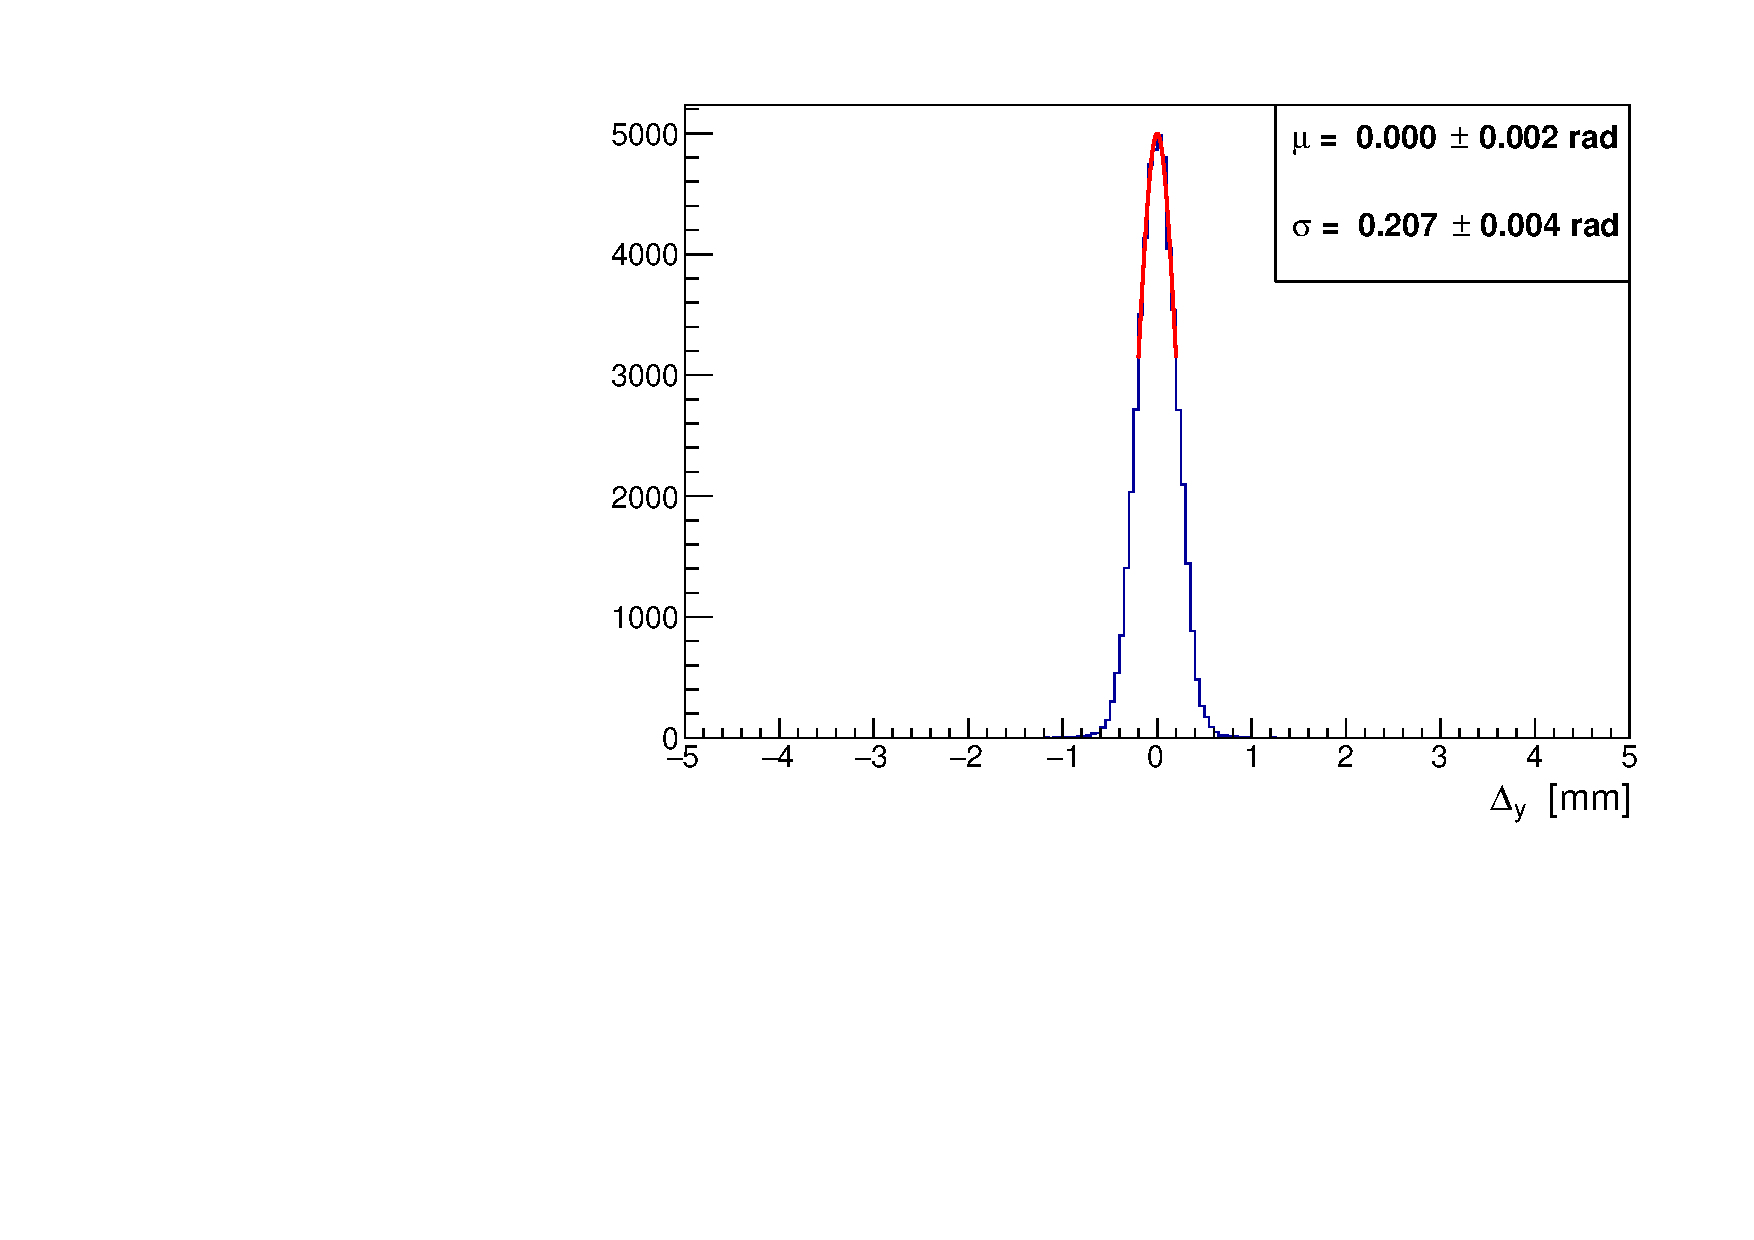
\includegraphics[width=0.49\textwidth, angle=0]{08-Performance/upstream_y_residual.pdf}
      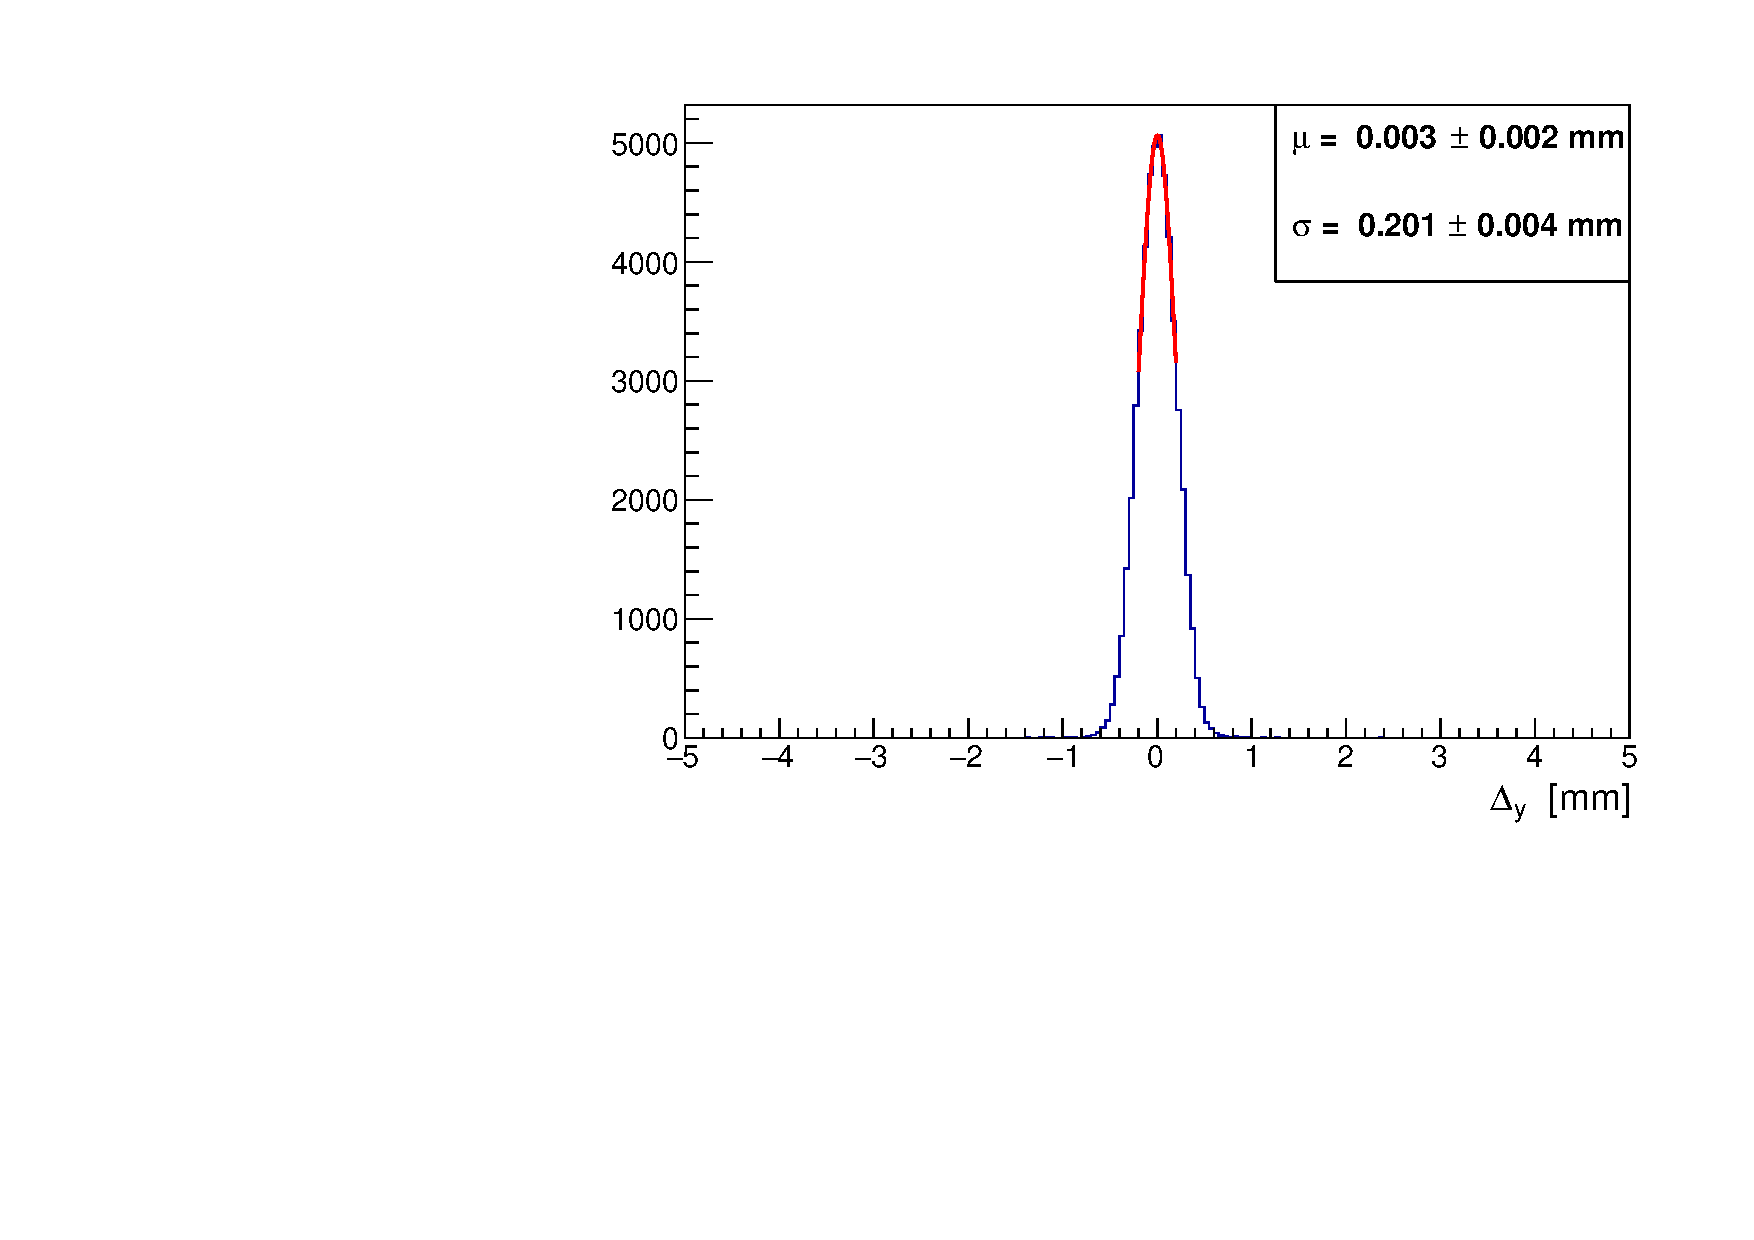
\includegraphics[width=0.49\textwidth, angle=0]{08-Performance/downstream_y_residual.pdf}
      \caption{\label{fig:YResidKalman} The $y$ residuals of the upstream (left) and downstream (right) trackers.}
    \end{center}
  \end{figure} 
  
  \begin{figure}[p]
    \begin{center}
      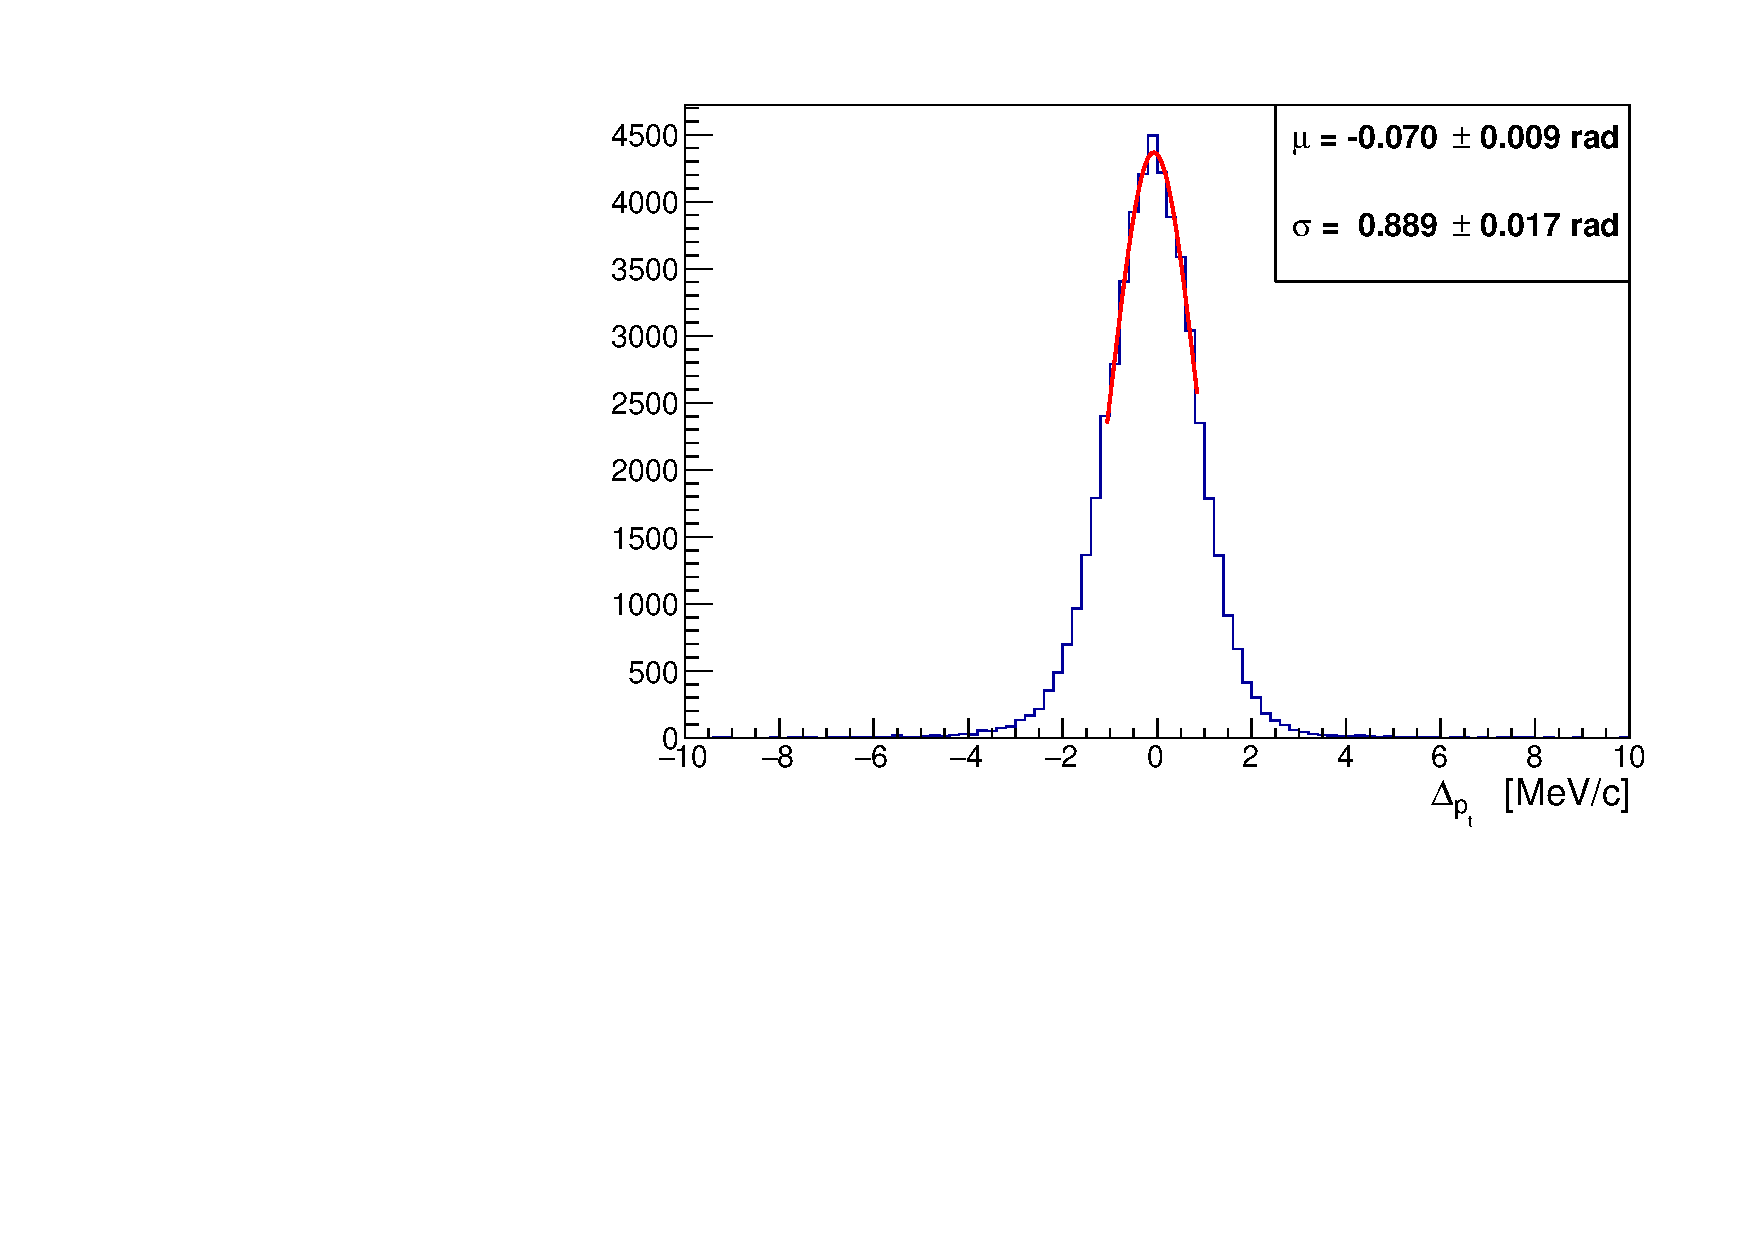
\includegraphics[width=0.49\textwidth, angle=0]{08-Performance/upstream_pt_residual.pdf}
      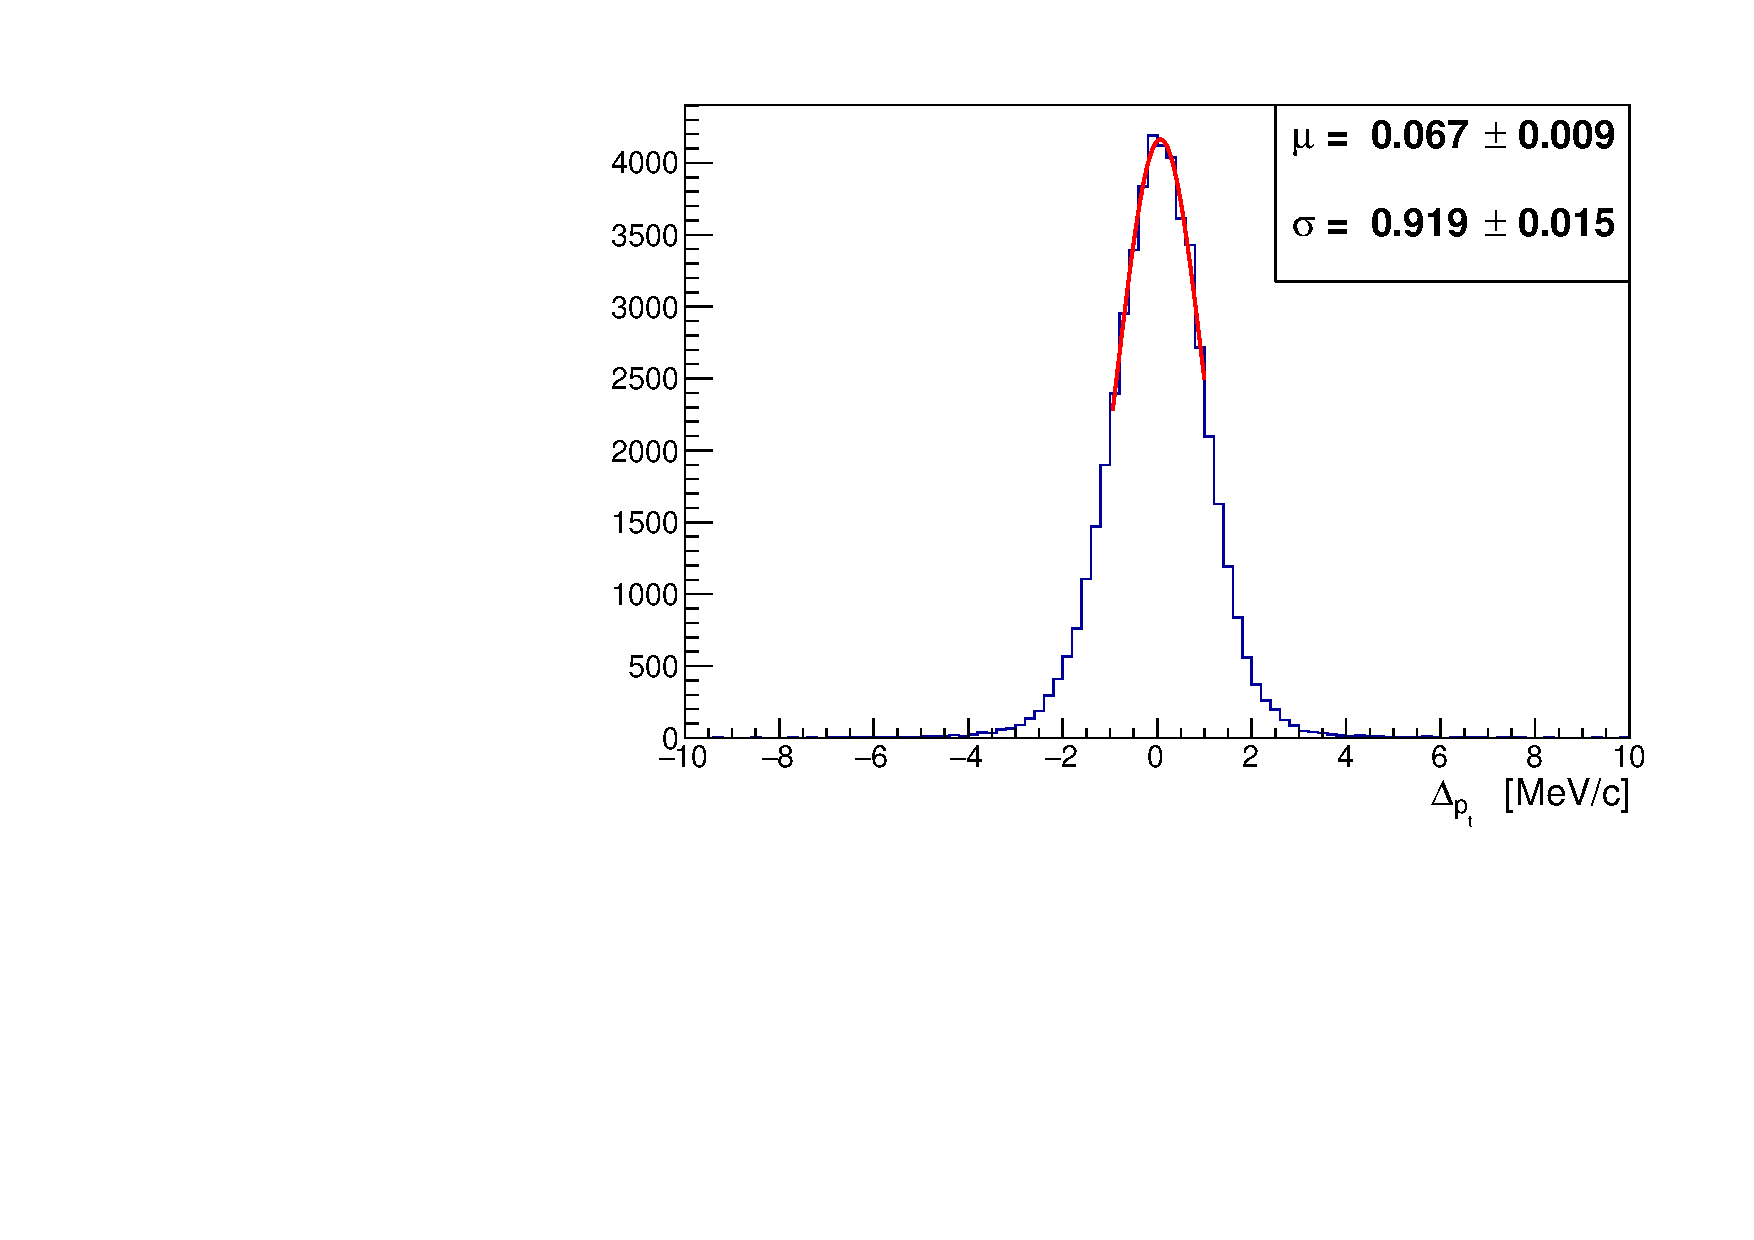
\includegraphics[width=0.49\textwidth, angle=0]{08-Performance/downstream_pt_residual.pdf}
      \caption{\label{fig:PtResidKalman} The $p_{t}$ residuals of the upstream (left) and downstream (right) trackers.}
    \end{center}
  \end{figure}
  
   \begin{figure}[p]
    \begin{center}
      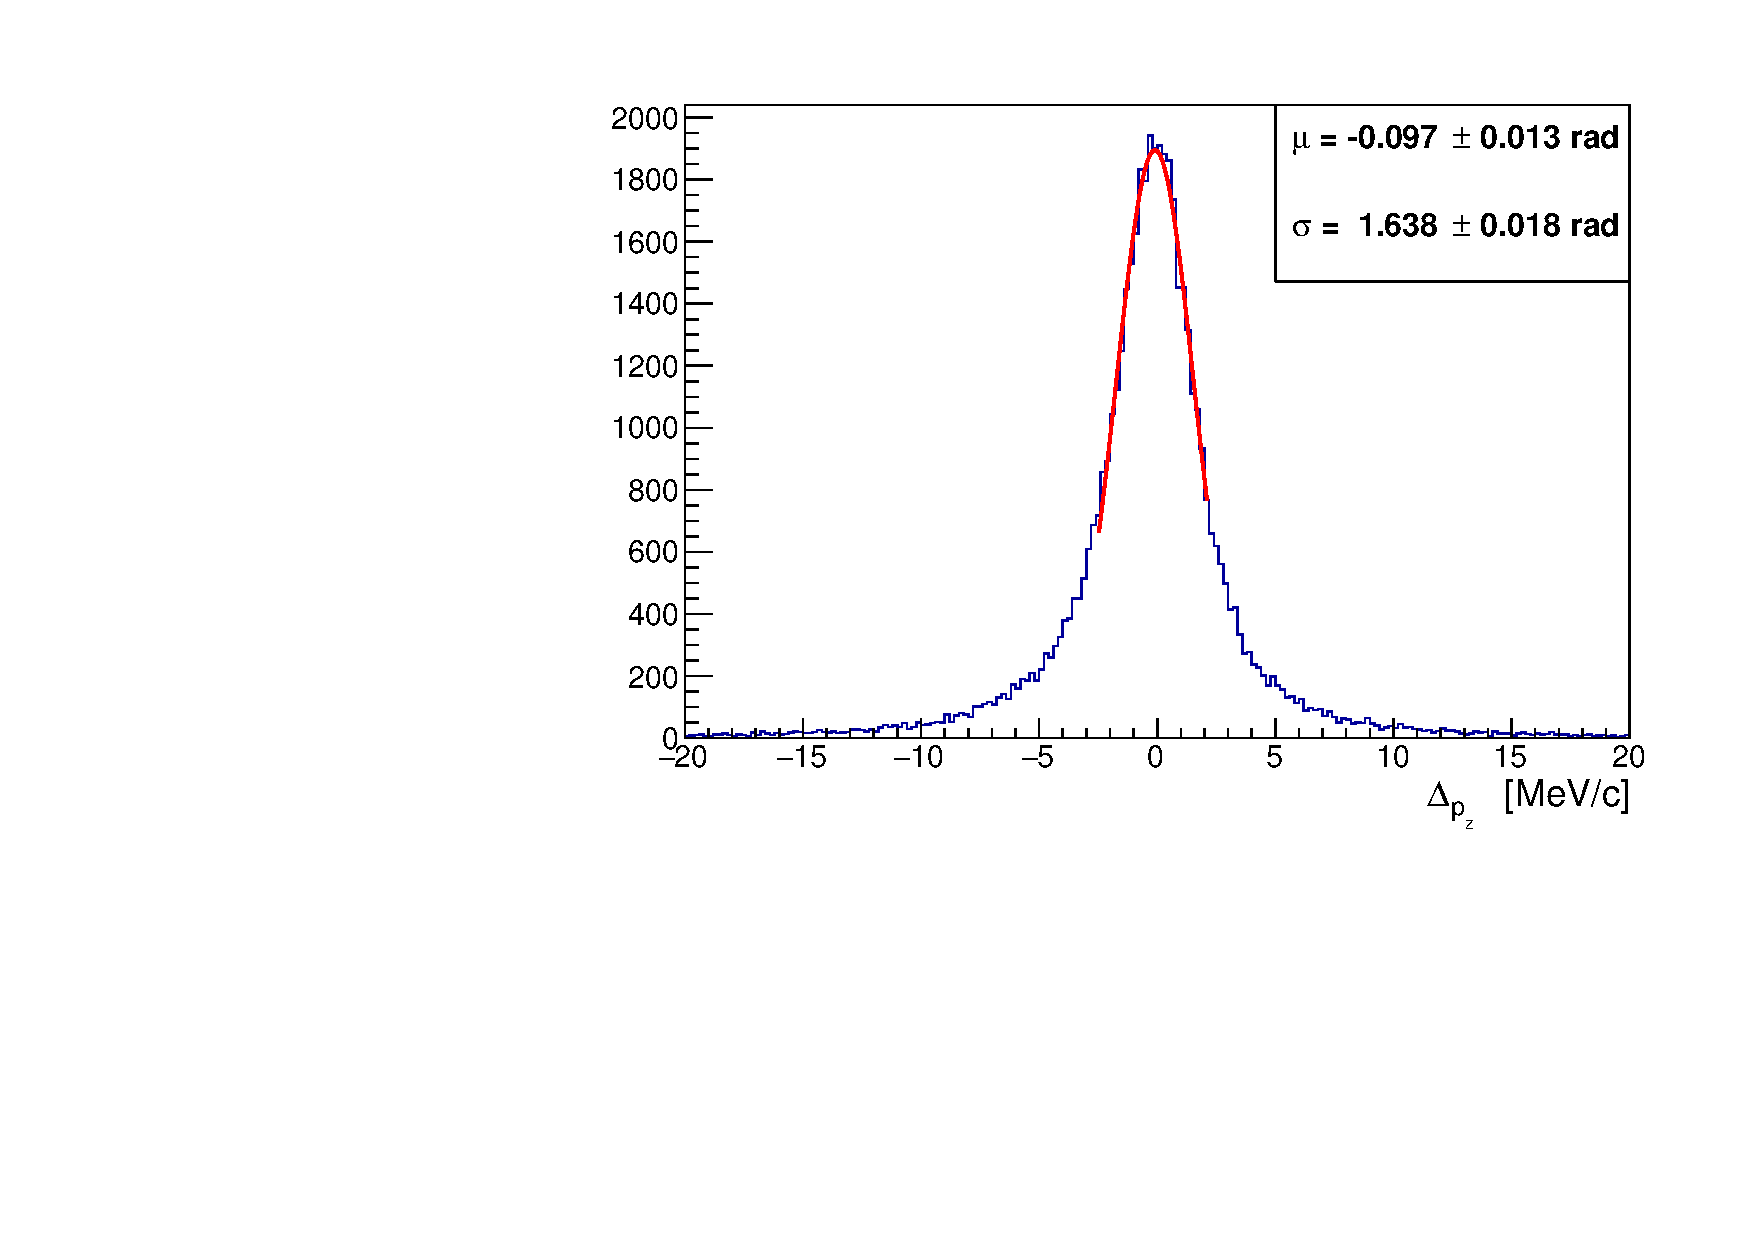
\includegraphics[width=0.49\textwidth, angle=0]{08-Performance/upstream_pz_residual.pdf}
      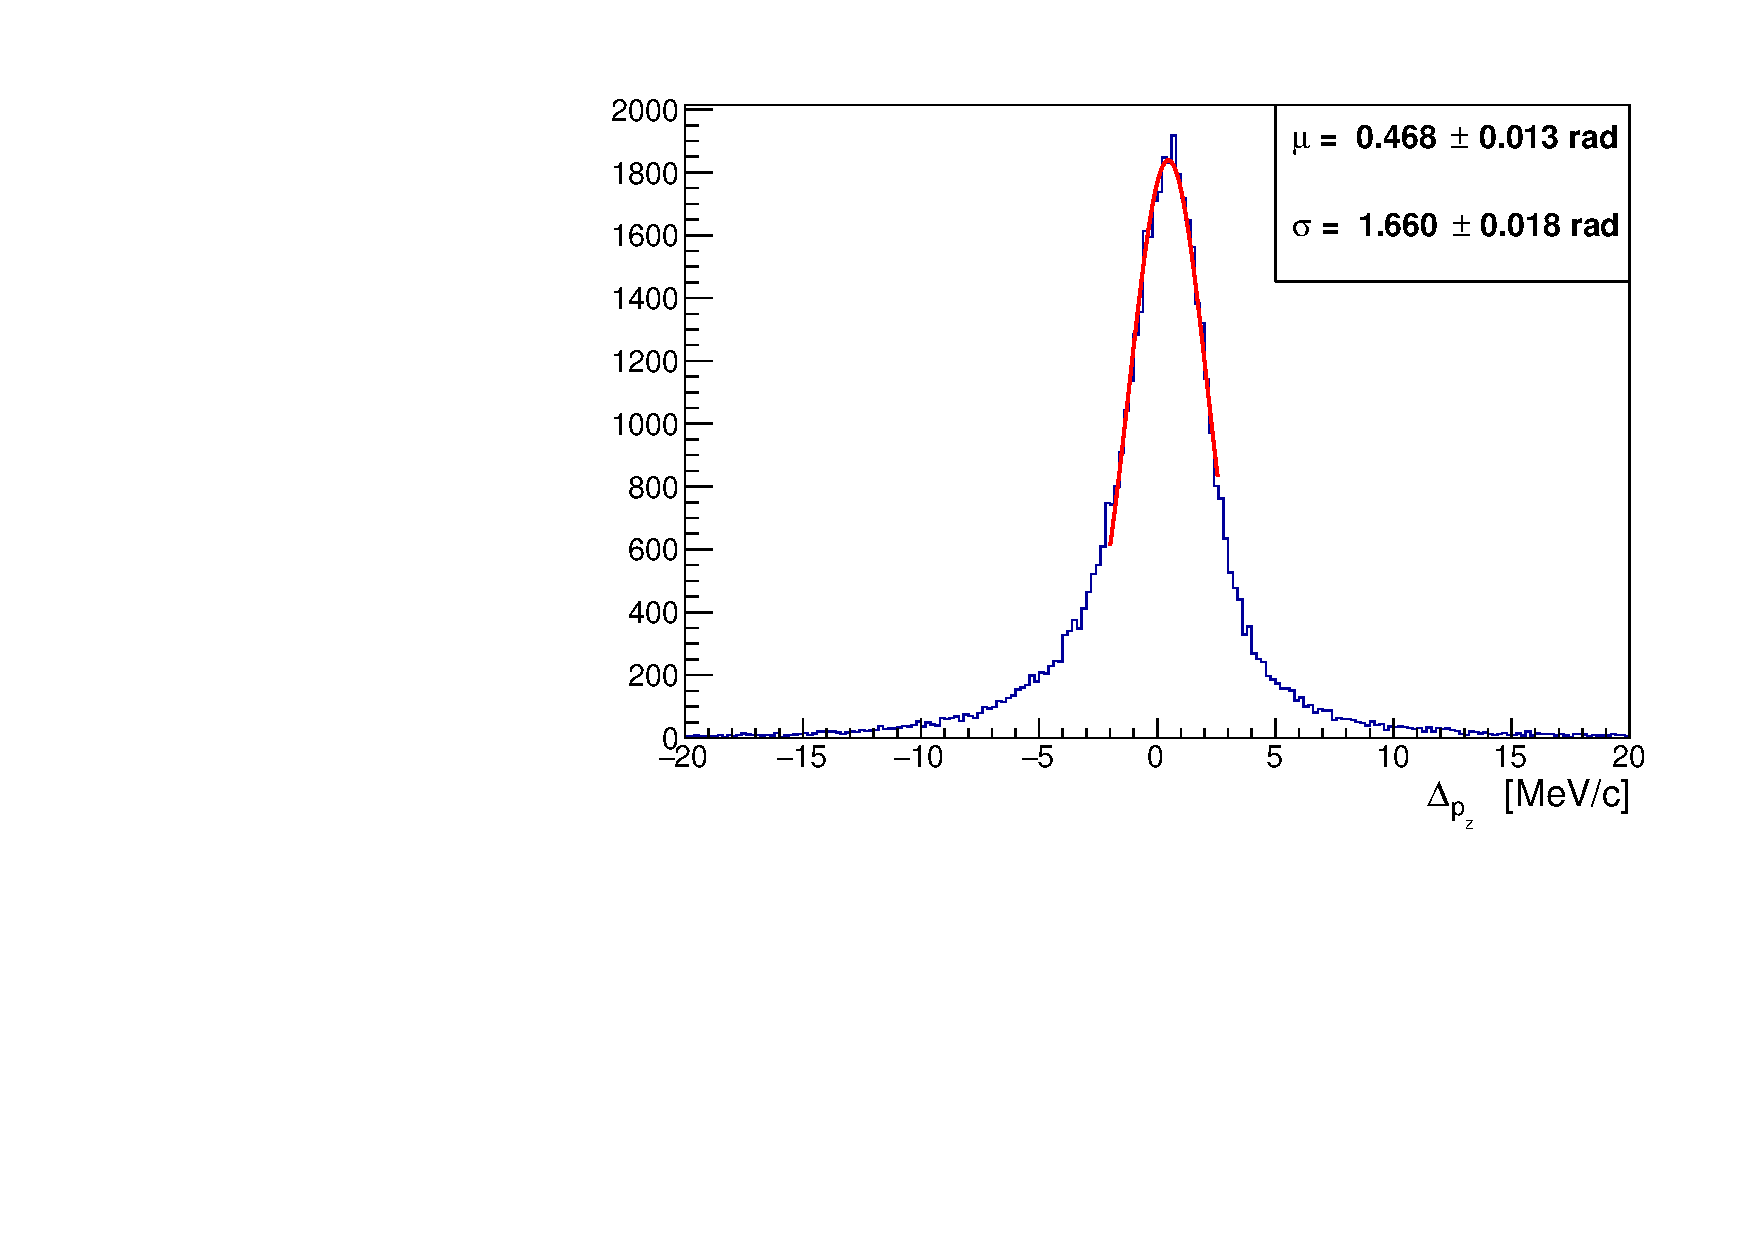
\includegraphics[width=0.49\textwidth, angle=0]{08-Performance/downstream_pz_residual.pdf}
      \caption{\label{fig:PzResidKalman} The $p_z$ residuals of the upstream (left) and downstream (right) trackers.}
    \end{center}
  \end{figure}
  
%   \begin{figure}[p]
%     \begin{center}
%       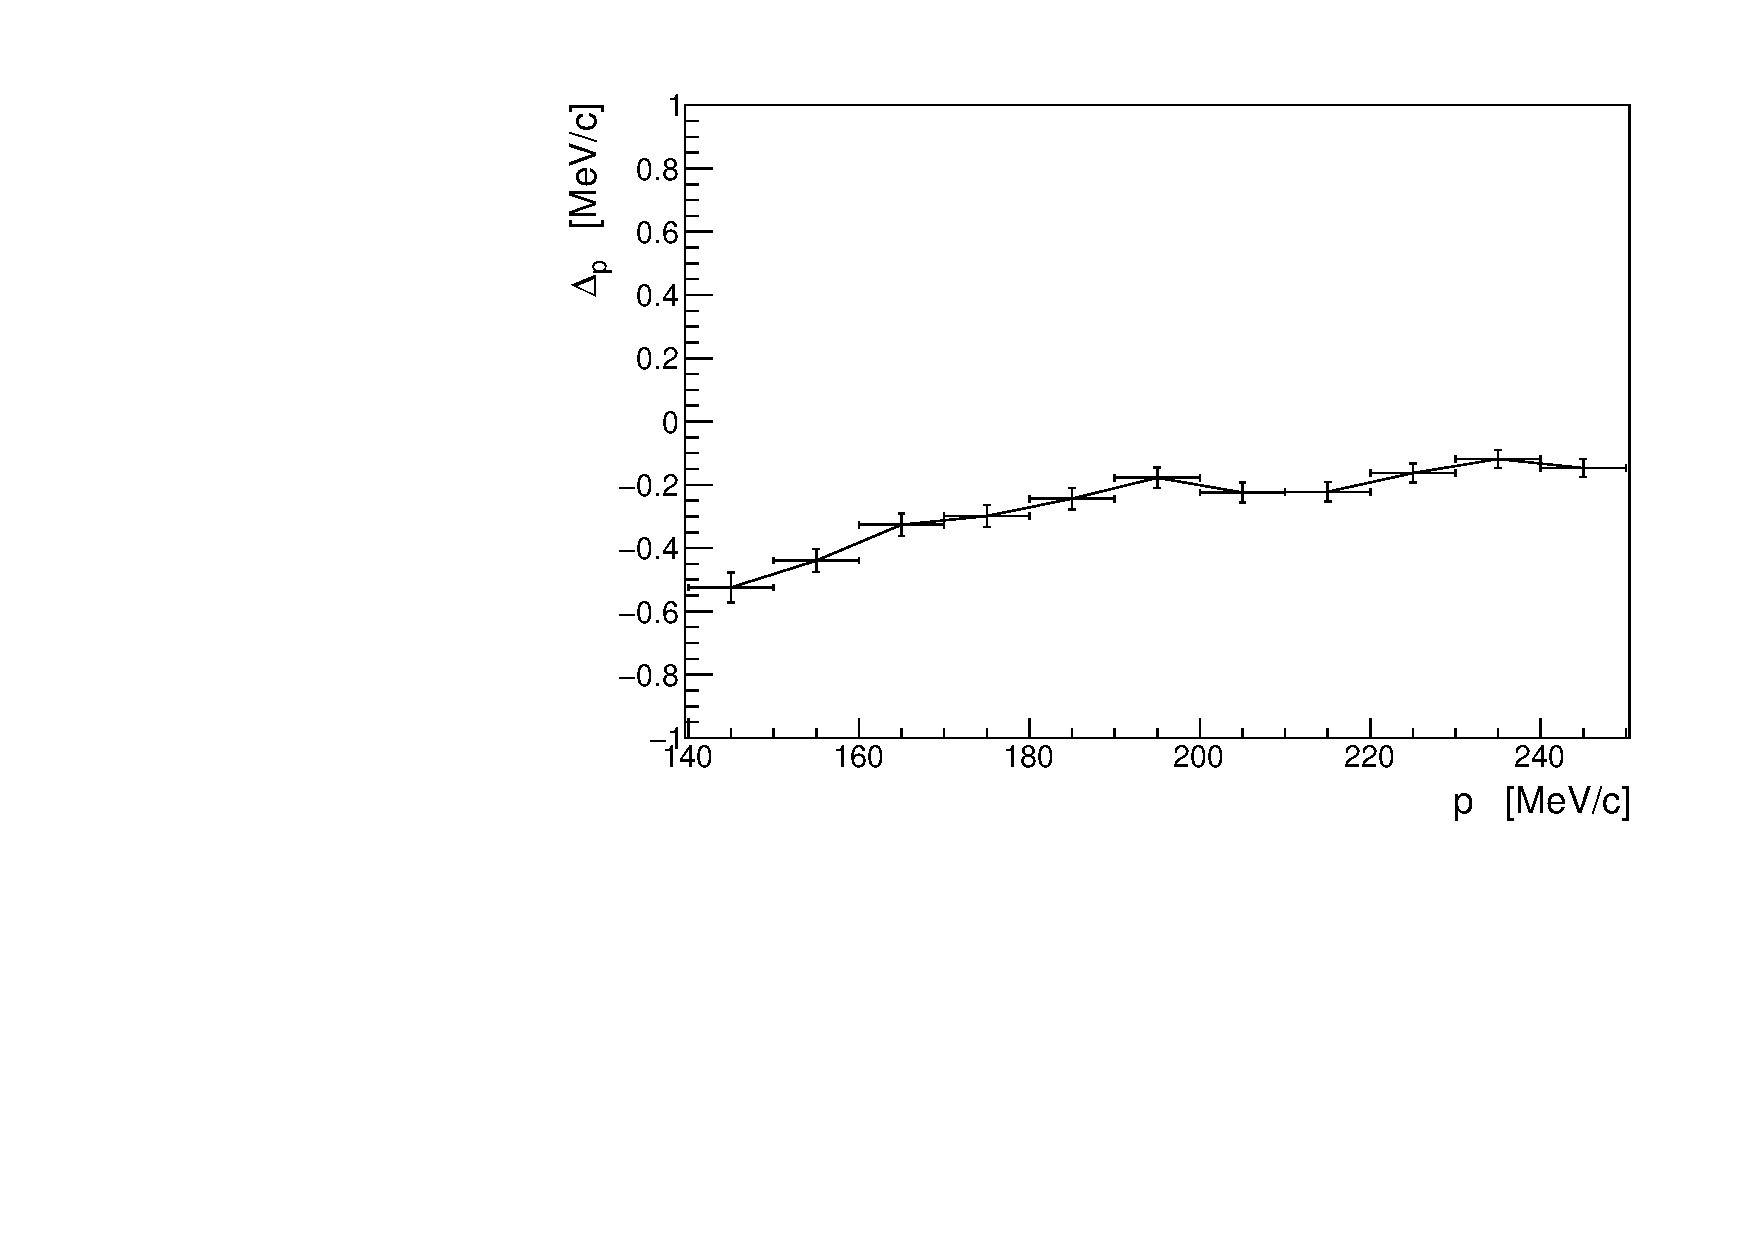
\includegraphics[width=0.49\textwidth, angle=0]{08-Performance/upstream_p_bias_p.pdf}
%       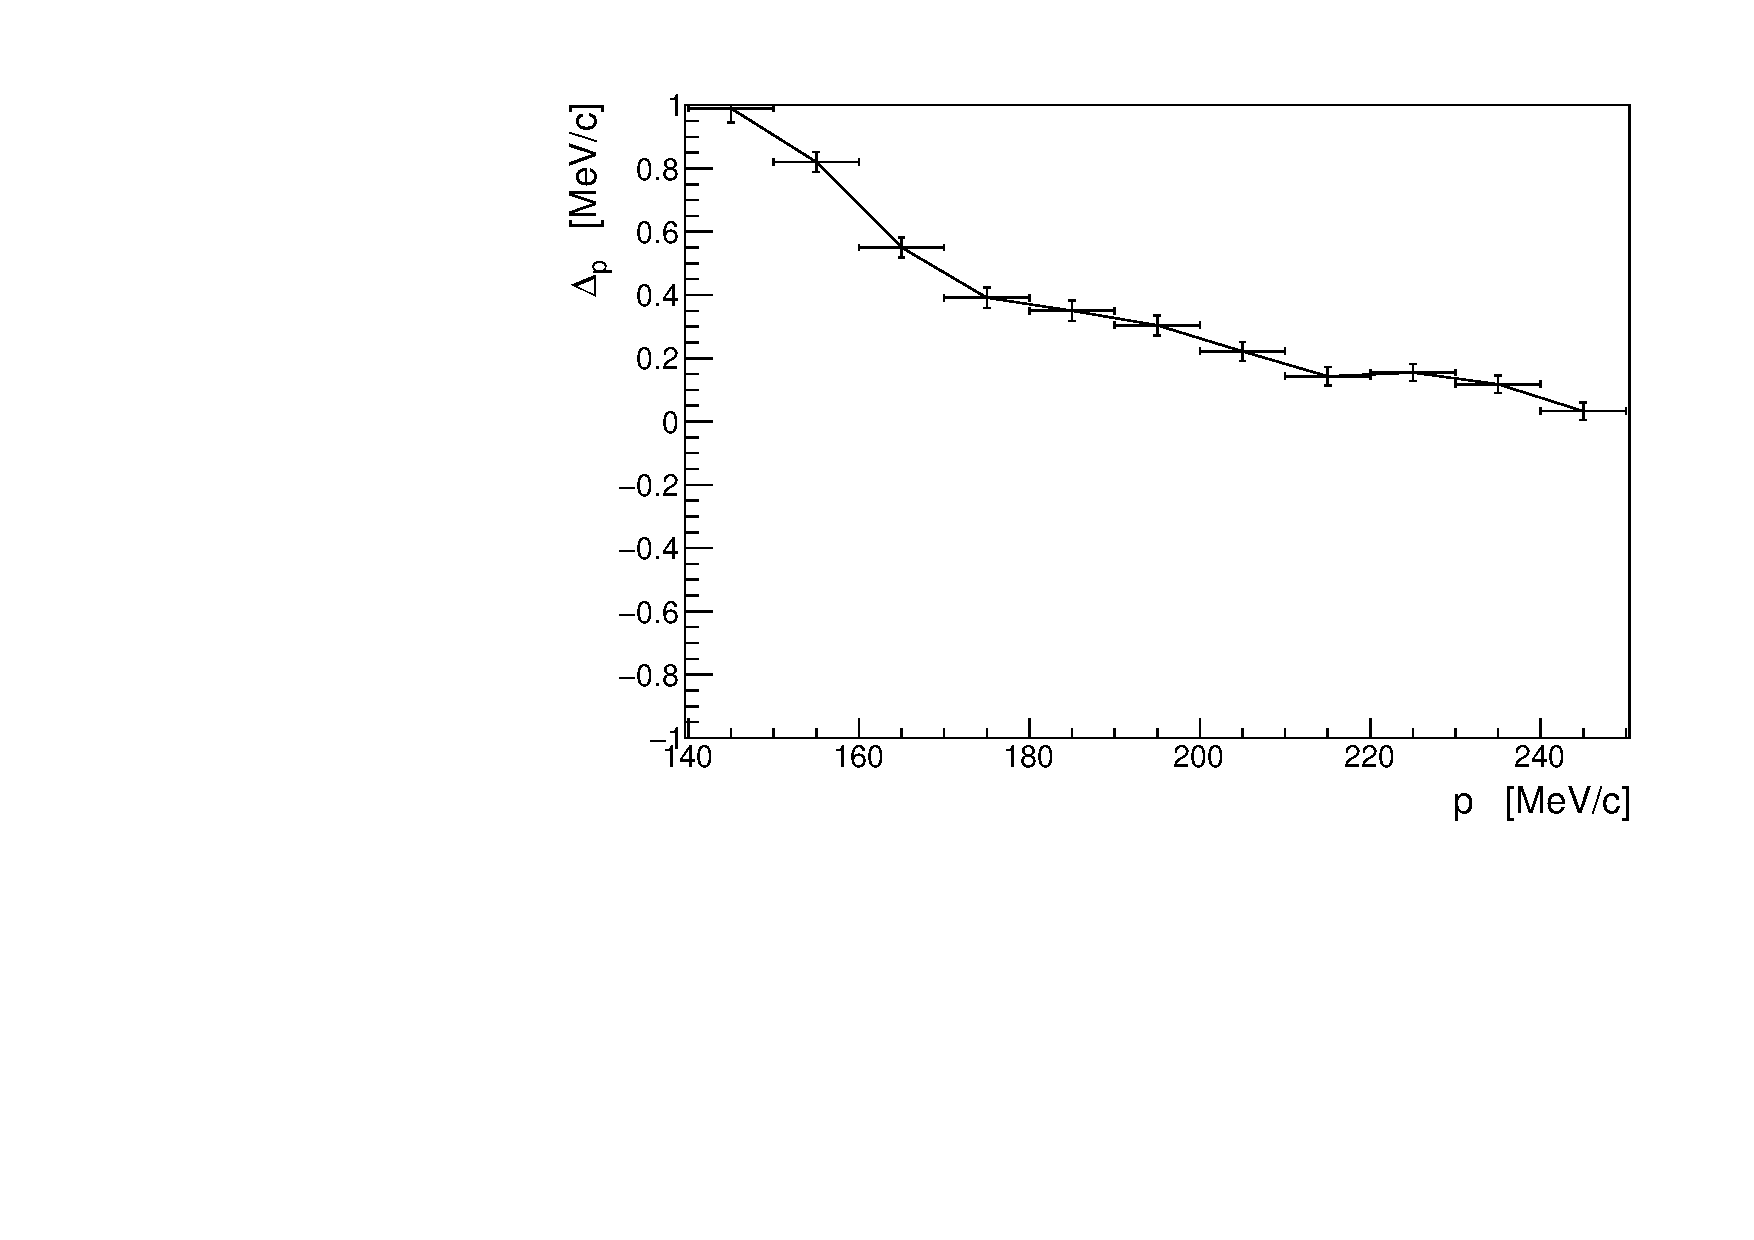
\includegraphics[width=0.49\textwidth, angle=0]{08-Performance/downstream_p_bias_p.pdf}
%       \caption{\label{fig:pBiasKalman} The mean residual between the final track fit total momentum and the true track momentum, evaluated at the reference plane.}
%     \end{center}
%   \end{figure}
  
  \begin{figure}[p]
   \begin{center}
     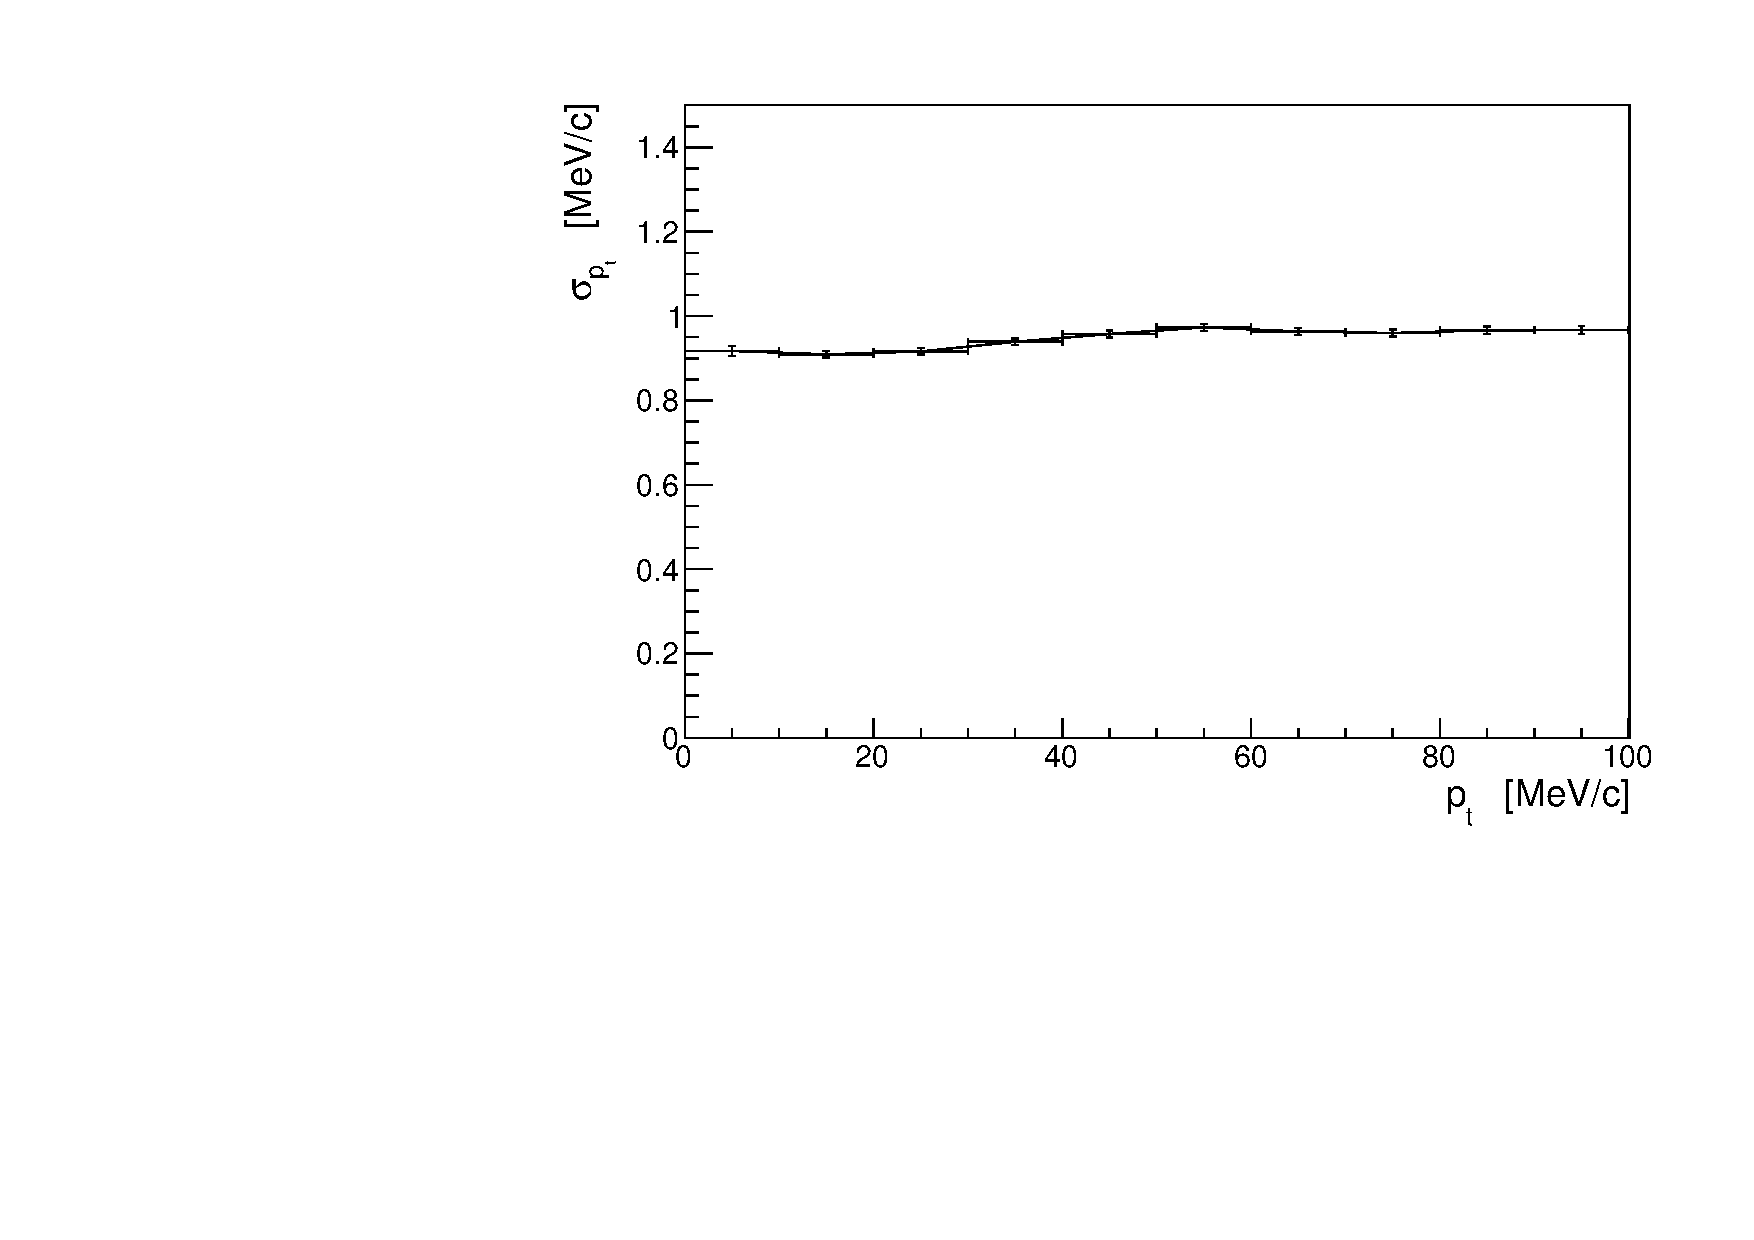
\includegraphics[width=0.49\textwidth, angle=0]{08-Performance/upstream_pt_resolution_pt.pdf}
     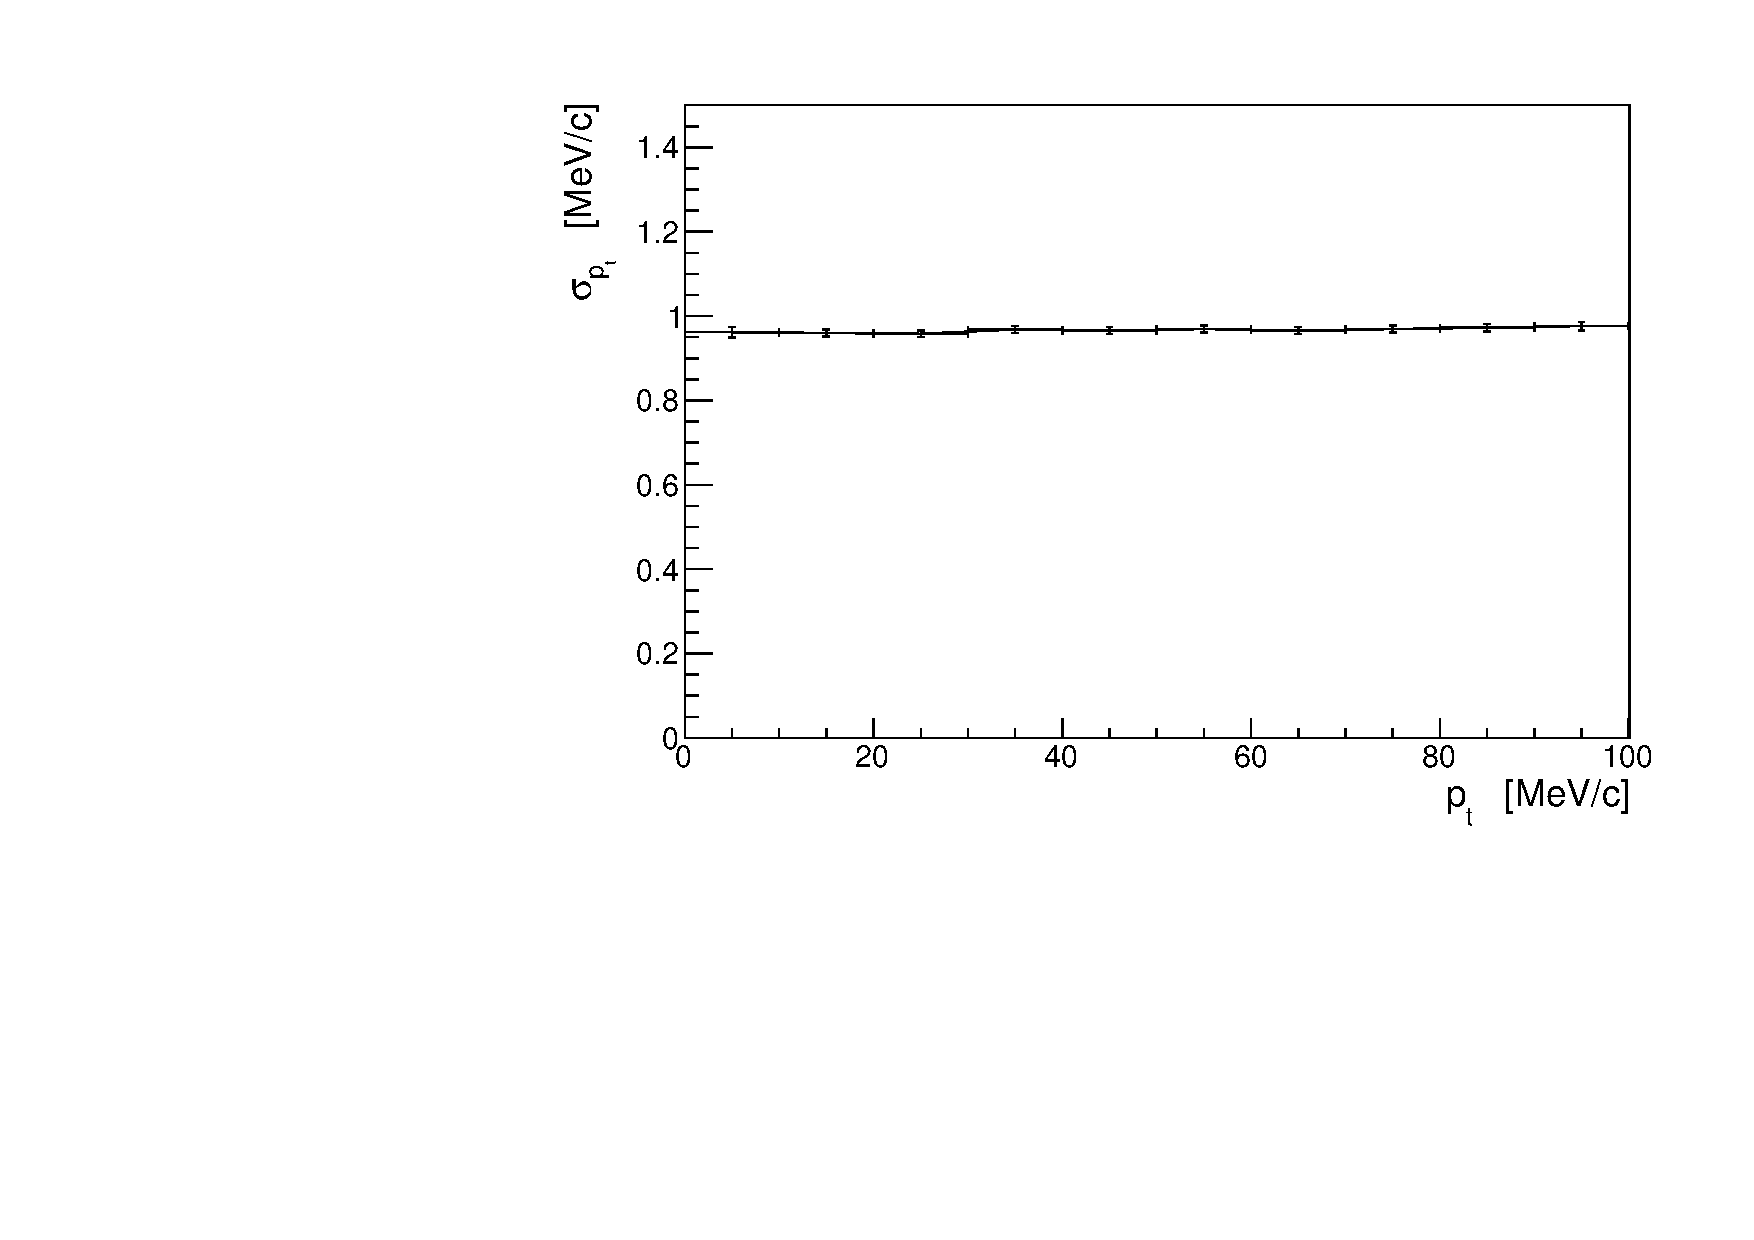
\includegraphics[width=0.49\textwidth, angle=0]{08-Performance/downstream_pt_resolution_pt.pdf}
     \caption{\label{fig:PtPtResolKalman} The $p_{t}$ resolution as a function of the $p_{t}$ of the upstream (left) and downstream (right) trackers.}
   \end{center}
  \end{figure}
  
  \begin{figure}[p]
   \begin{center}
     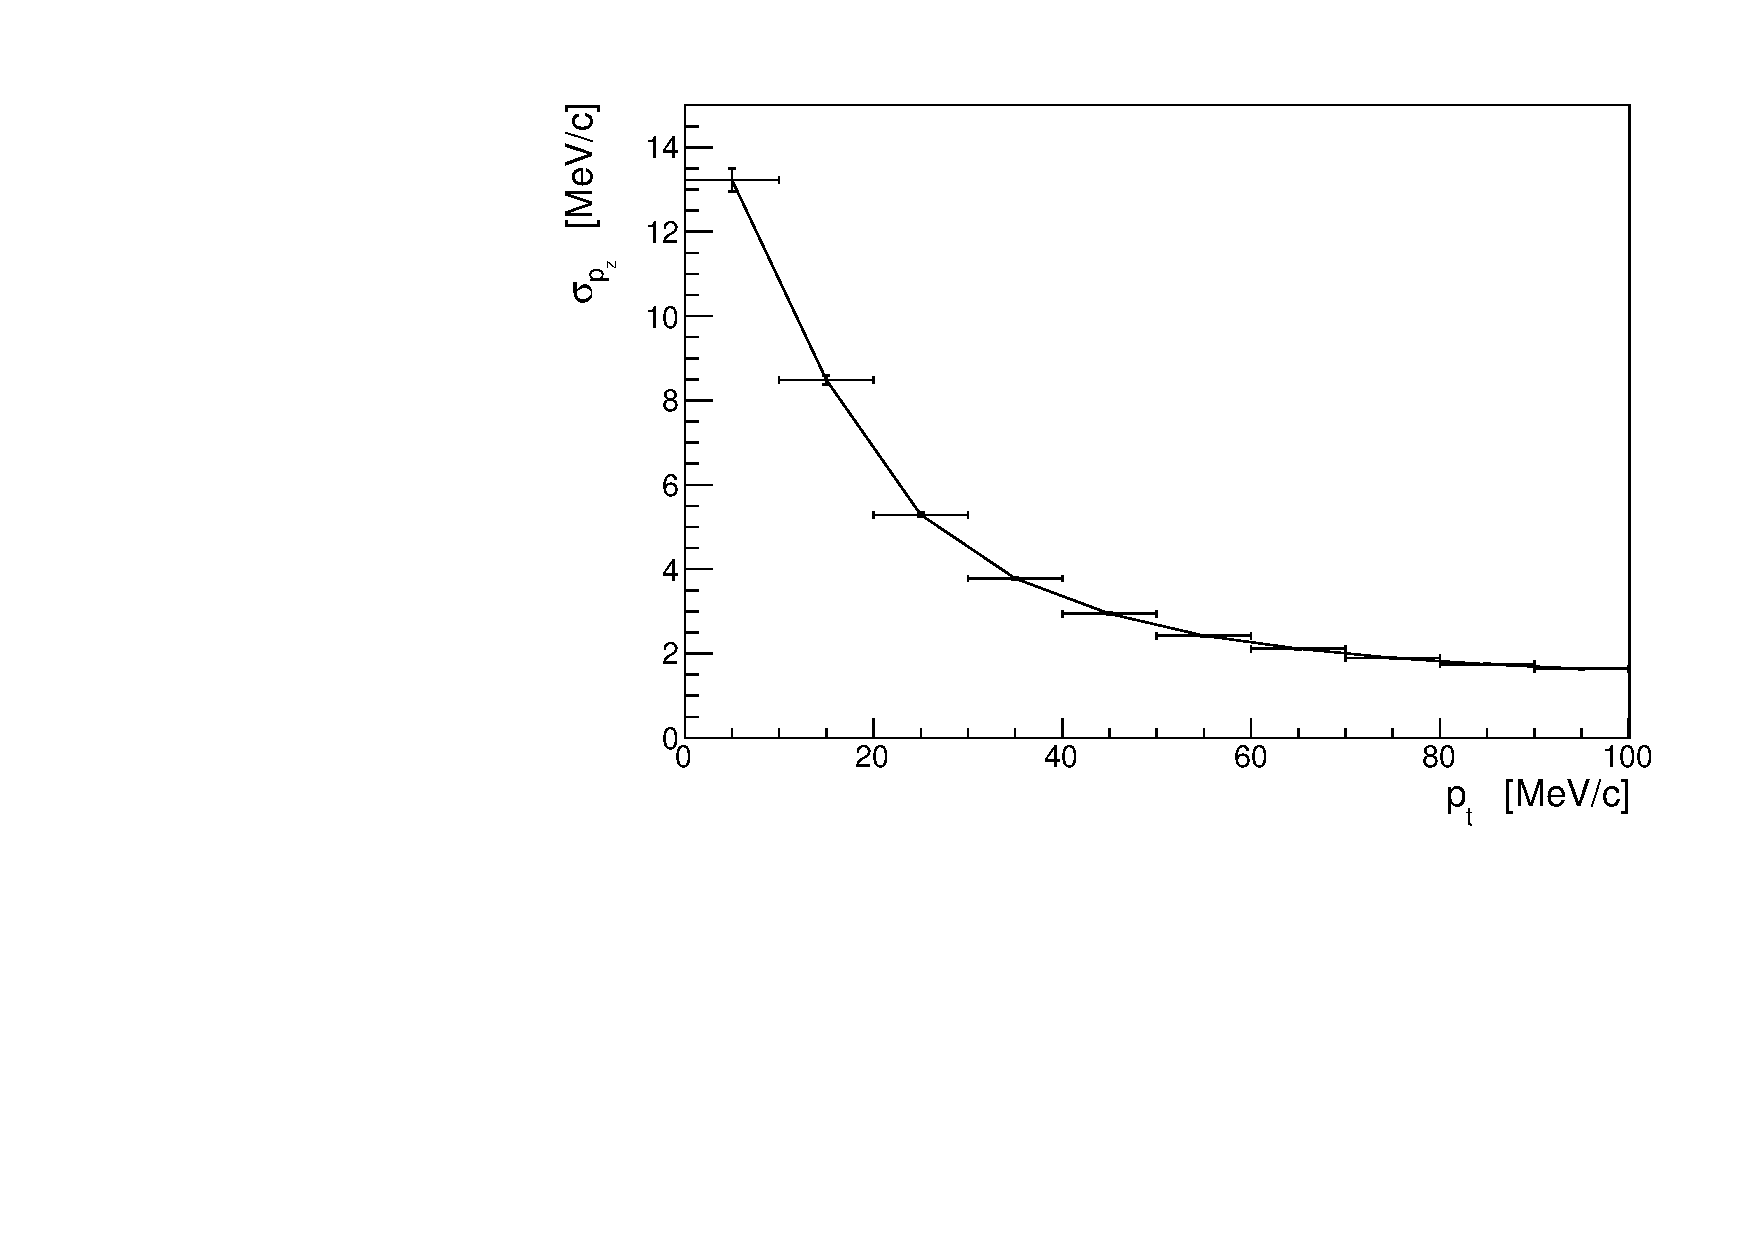
\includegraphics[width=0.49\textwidth, angle=0]{08-Performance/upstream_pz_resolution_pt.pdf}
     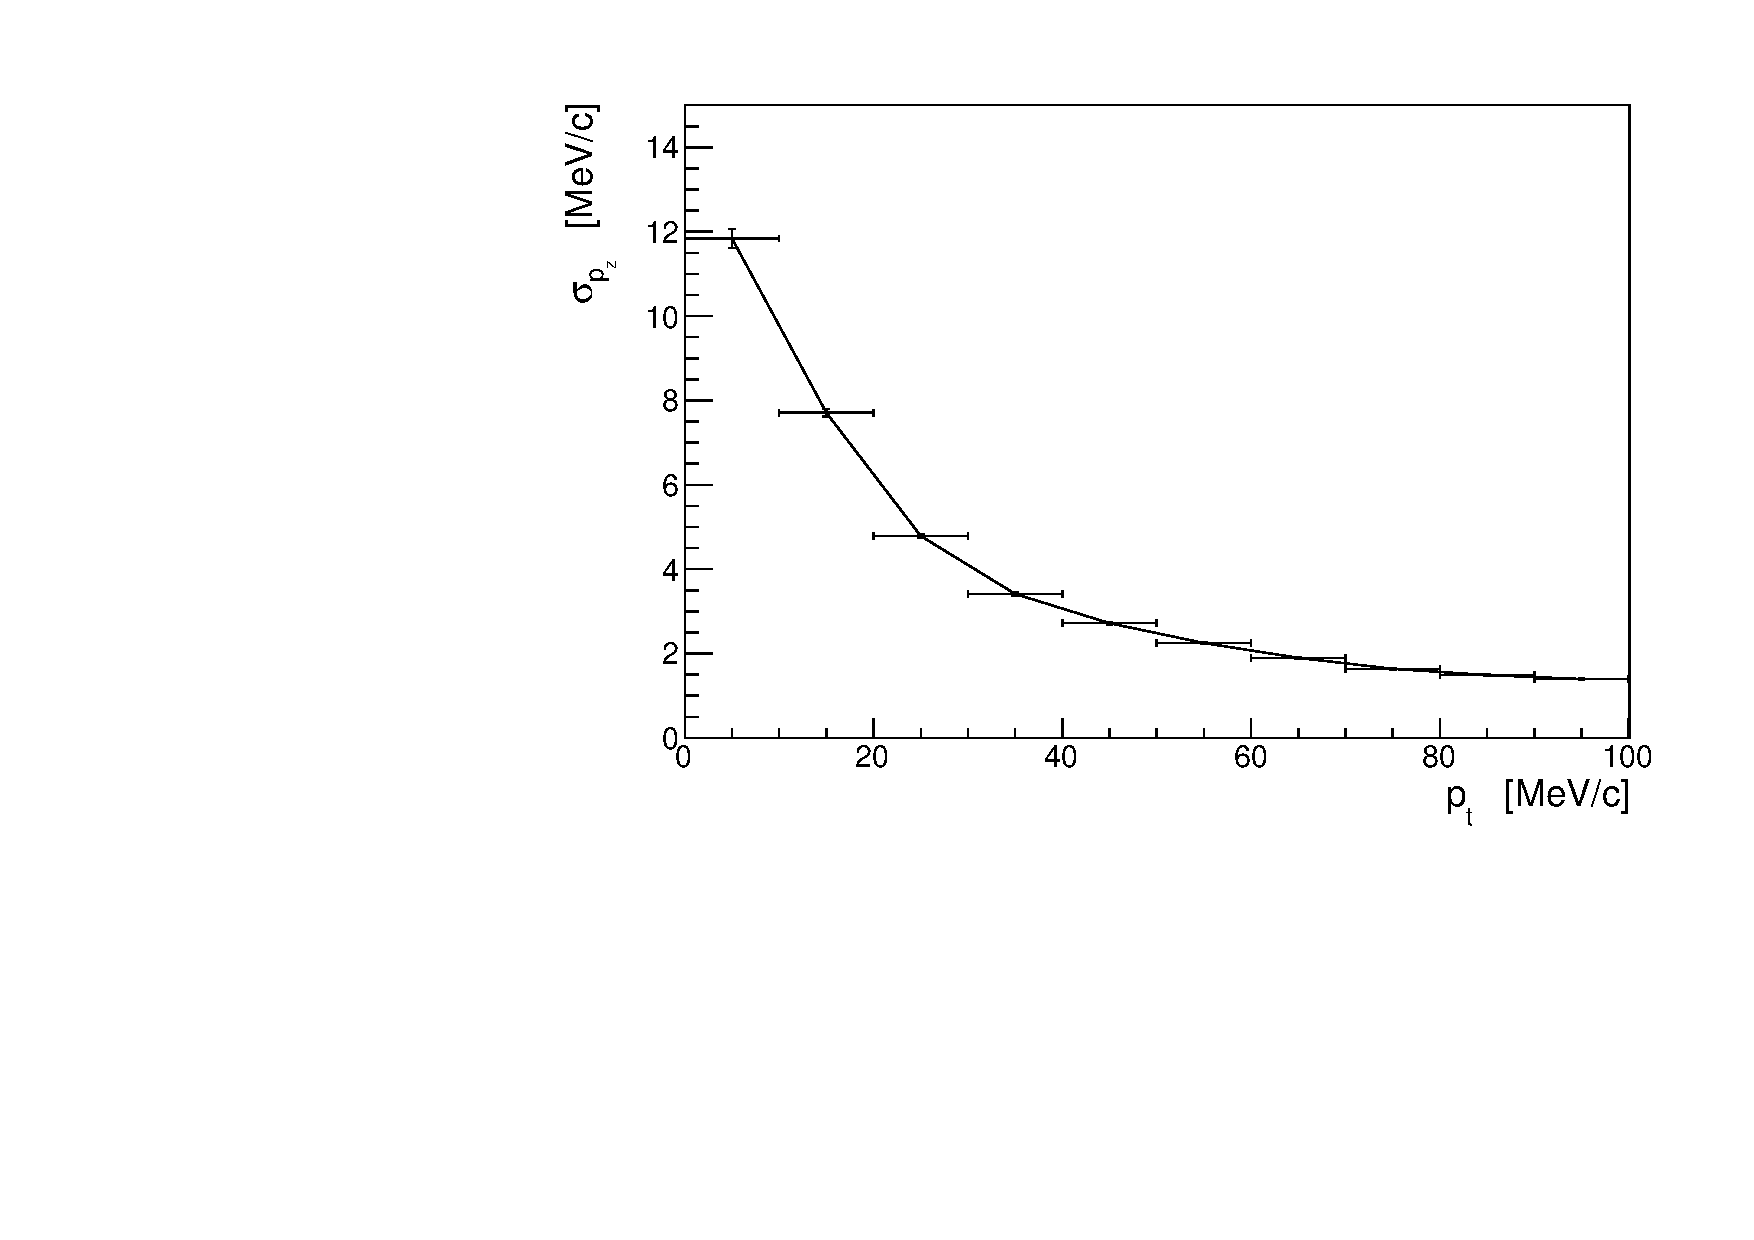
\includegraphics[width=0.49\textwidth, angle=0]{08-Performance/downstream_pz_resolution_pt.pdf}
     \caption{\label{fig:PtPzResolKalman} The $p_z$ resolution vs the $p_{t}$ of the upstream (left) and downstream (right) trackers.}
   \end{center}
  \end{figure}

\section{Acknowledgements}
\label{sec:Acknowledgements}

The work described here was carried out in the context of the international Muon Ionization Cooling Experiment. It was made possible by grants from Department of Energy and National Science Foundation (USA) and the Science and Technology Facilities Council (UK). We gratefully acknowledge all sources of support.

We are also grateful to the staff of the ISIS Department at the Rutherford Appleton Laboratory for the reliable operation of ISIS. We acknowledge the use of Grid computing resources deployed and operated by GridPP in the UK, http://www.gridpp.ac.uk/.

%\clearpage

\bibliography{mice}                                                                           
\bibliographystyle{99-Styles/utphys}


% \cleardoublepage
% \appendix

\end{document}
